\documentclass[10pt,a5paper]{book}
\usepackage[utf8]{inputenc}
\usepackage{amsmath}
\usepackage{amsfonts}
\usepackage{amssymb}
\usepackage[left=2cm,right=2cm,top=2cm,bottom=2cm]{geometry}
\begin{document}
\title{Linux'a Giriş}
\author{Z.Tuğçe Şirin\\
Mithat Göğebakan\\
Samet İlhan\\
Serdar Orazmamedov\\
Özcan Zafer Ayan\\
Emre Doğru\\
Sena Özben\\
Margulan Byekmurat\\
Sema Özvin\\
Ahmet Dellal\\
Emrah Şentürk\\
Ebru Akagündüz}
\renewcommand{\today}{December 13, 2012}
\renewcommand*\chaptername{Bölüm}
\maketitle
Linux Essentials is a new certification by the Linux Professional Institute (LPI) which is aimed especially at schools and universities in order to introduce children and young adults to Linux
\renewcommand*\contentsname{İçindekiler}
\tableofcontents
\listoftables
\chapter{Bilgisayarlar, Yazılım ve İşletim Sistemleri}
\label{chap:bolum1}
\paragraph{Amaçlar}
\begin{itemize}
 \item Temel bilgisayar donanım bilgisini edinmek
 \item Farklı işletim sistemlerinin farkında olmak ve bu sistemlerin farklı yönleri ile benzer yönlerini tayin etmek
 \end{itemize}
 
\paragraph{Önceden Bilinmesi Gerekenler}
\begin{itemize}
 \item Temel bilgisayar bilgisi işe yarar olacaktır.
 \end{itemize}

\begin{section}{Bilgisayar da neyin nesi?}
Bilgisayarın ne olduğunun ayrıntılarına girmeden önce, bilgisayar camiasının dikkate değer kişilerinden birkaç alıntı ile işe başlayalım.
\begin{quote}{Esasında Birleşik Devletler'de, gizlenmiş araştırma laboratuvarlarında yarım düzine kadar büyük bilgisayarlardan olsaydı; bu, ülke olarak ihtiyaç duyduğumuz şeylerin çaresine bakabilirdi. Howard H. Aiken, 1952}
\end{quote}
Howard Aiken bilgisayar alanında bir öncüydü ve IBM' nin ilk bilgisayarı "Harvard Mark I"in tasarımcısıydı. Modern anlayışa göre inşaa edilmiş ilk bilgisayarlar İkinci Dünya Savaşında şifrelenmiş mesajları deşifre etmek için ya da zor hesaplamaları yapmak için yapılmıştı; büyük, karmaşık ve hataya yatkınlardı. Bugünlerde bilgisayarlarda bulunan transistör ya da entegre devreler henüz icat edilmemişti. Bu zamanlarda aydınlığa kavuşan şey, savaşın hemen sonrasında ortaya çıkan bir takım temel varsayımlarla oluşturulan "bilgisayar" olarak kabul edilebilecek bir cihazın varlığıydı.
\begin{itemize}
 \item Bilgisayar veriyi 'otomatik olarak' çalıştırılan komutların sırasına göre işler,
 \item Programlar şartlı çalışmalara ve döngülere izin vermelidir,
 \item Bilgisayarın çalıştırdığı programı değiştirmek veya yerine başka bir şey yerleştirmek mümkün olmalıdır
 \end{itemize}

Örnek olarak, çoğu teknolojik cihaz - televizyon setlerinden dijital kameralara çamaşır makinesine ya da arabalara kadar - bugünlerde neredeyse küçük bir bilgisayar sayılabilecek programlanmış kontrol birimleri içerir. Böyle olmasına rağmen bu cihazları "bilgisayar" olarak görmeyiz, çünkü bu cihazlar sadece düzenlenmiş ve değiştirilemez programları çalıştırırlar.  Buna karşın bir hesap makinesi "verileri işlemek" için kullanılabilir ama - eğer "programlanabilir bir hesap makinesi" kadar pahalı değilse - bu otomatik olarak olmaz; bir insan tuşlara basmalıdır.

1950'nin başlarında, bilgisayarlar insanların ancak araştırma kurumlarında görmeyi bekleyeceği – Aiken'in öngördüğü gibi - yüksek derecede özelleştirilmiş cihazlardı. Zamanın bilim -kurgu filmleri gizemli dönen çarklarla dolu dolapların olduğu koridorları gösteriyordu. Tam olarak 70 yıl bile olmadan bu görüntü önemli bir ölçüde değişti. 
\footnote{Bu metinde belirtilen alıntının aslında Thomas J. Watson, IBM'in CEO'su, 1943'te “Dünya pazarında sadece beş bilgisayar için yer vardır.” sözleriyle birlikte söylendiği tasvir edilir. Ne yazık ki bu hiçbir zaman doğrulanamamıştır. Ve eğer 1943'te gerçekten bunu söylediyse, bu en azından 10 yıl için geçerli olurdu.}
\begin{quote}
{Kimsenin evinde bir bilgisayara sahip olmasına gerek yoktur. Ken Olsen, 1977}
\end{quote}

Ken Olsen bir bilgisayar üreticisi olan ve 1970' lerdeki “küçük” kavramının “havalandırmalı bir makine odasına ve güç ünitesine ihtiyaç duymayan ve bir milyon dolardan daha ucuza mal olan” anlamına geldiği zamanlarda “küçük” bilgisayarların geliştirilmesinde öncü bir firma olan  DEC (Digital Equipment Corporation) \footnote{DEC 1998 yılında Compaq tarafından alındı, Compaq ise 2002' de Hewlett-Packard tarafından alındı.} firmasının yöneticisi idi. Donanım teknolojisinin gelişmesiyle 1970'lerin sonuna doğru “küçük” kavramı “iki insan tarafından taşınabilir” anlamına gelmeye başladı.

DEC Linux camiası için önemlidir çünkü Unix - kendi oluşumundan 20 yıl sonra Linus Torvald'a Linux'u başlatmak için ilham veren sistem - ilk olarak DEC PDP-8 ve PDP-11 bilgisayarları üzerinde geliştirilmiştir.

Ayrıca 1970'ler ilk “ev bilgisayarları”nın varlığını gördü. Bu günümüzün kişisel bilgisayarlarıyla karşılaştırılamaz çünkü insanlar evde kendileri bilgisayarlarını lehimlemek durumundaydı (ki bu zamanlarda fiziksel olarak imkansız bir durum olurdu) ve bu bilgisayarlar çok nadir olarak kullanılabilir bir klavye ve iyi bir ekran ile geliyordu. Bu bilgisayarlar genellikle bir tamircinin eski kullandığı malzemelerden yapılıyordu, bir elektrikli tren setinden geriye kalanlar gibi, çünkü gerçekte çok kullanışlı değillerdi. Buna rağmen, bizim önceden yaptığımız tanımımıza göre “bilgisayar” olarak adlandırılıyorlardı çünkü özgürce programlanabiliyorlardı, bu zahmetli bir şekilde her şeyi tuşlardan girmek ya da (eğer o kadar şanslıysanız) bir ses kaset teypinden yüklemek anlamına gelse bile. Yine de bu bilgisayarlar tümüyle ciddiye alınmıyorlardı ve Ken Olsen'in cümlesi sık sık yanlış yorumlandı. O hiçbir şekilde küçük bilgisayarlara karşı değildi (hatta işi bu bilgisayarları satmaktı). Onun anlamadığı şey bütün ev işlerinin (ısıtma, aydınlatma, eğlence ve bunun gibi şeyler) bir bilgisayar tarafından kontrol edilmesi fikriydi – bu fikir o zamanlar sadece teoride vardı ama günümüzde oldukça uygulanabilir bir durumda.

1970'lerin  sonunda ve 1980'lerde “ev bilgisayarları” parçalar topluluğundan kullanmaya hazır  cihazlara (“Apple II” ya da “Commodore 64” gibi isimler hala bu işin içinde olan eski üyelerimize tanıdık gelebilir) dönüştü ve ofislerde de bu cihazlardan bulunmaya başladı. IBM tarafından ilk kişisel bilgisayar 1981'de duyruldu ve Apple ilk “Macintosh”u 1984'te piyasaya sundu. Bunların dışındakiler, söylenildiği gibi, tarihte kaldı ama bilgisayar dünyasının sadece kişisel bilgisayarlardan ya da Mac' lerden oluşmadığı unutulmamalıdır.  Devasa, odaları dolduran eski bilgisayarlar hala bulunmaktadır ama bu durum gitgide azalmakta ve büyük gruplarda günümüz bilgisayarlarından oluşmaktadır. Bununla birlikte temel ilke Howard Aiken'in zamanında beri değişmedi: Bilgisayarlar hala veriyi koşul ve döngüler içerebilen değişebilir programlara göre otomatik olarak işleyen cihazlardır. Ve işler bu şekilde yürümeye devam edecek gibi görünüyor. 

\paragraph{{\Huge{\PencilLeftDown}}Alıştırmalar}{
\begin{enumerate}
 \item İlk kullandığınız bilgisayar neydi? Ne çeşit işlemci içeriyordu, ne kadar belleği vardı ve sabit diski ne kadar büyüktü (eğer bir sabit diski bulunuyorduysa - eğer sabit diski bulunmuyorduysa veri nasıl kalıcı olarak depolanıyordu)?
\end{enumerate}}

\end{section}

\begin{section}{Bir Bilgisayarın Parçaları}

Hadi bir bilgisayarın (ya da daha açık olmak gerekirse IBM-uyumlu bir kişisel bilgisisayarın) içine bakma fırsatını yakalayalım ve burada bulmamızın mümkün olduğu parçaları inceleyelim:
\paragraph{İşlemci}{(“CPU” Türkçe anlamıyla “Merkezi İşlem Ünitesi”) bilgisayarın çekirdeğidir: burası bilgisayarı bilgisayar yapan, program kontrolündeki verilerin işlendiği yerdir. Bugünün işlemcileri genelde birkaç "çekirdek" içerir, bunun anlamı işlemcinin ana parçaları birden fazladır ve bağımsız olarak (bağımsız işlem yapabilme bilgisayarın işlem hızını ve buna bağlı olarak performansını arttırır) işlem yapabilirler.  Genelde hızlı bilgisayarlar birden fazla işlemci içerirler. Bilgisayarlar normalde Intel ya da AMD işlemcilerine (detaylarda farklılık gösterebilir ama aynı programları çalıştırabilirler) sahiptir. Tabletler ve akıllı telefonlar genel olarak ARM işlemcilerini kullanırlar. Bunlar diğerleri kadar güçlü değildirler ama enerjiyi daha az tüketirler. Intel ve AMD işlemcileri direkt olarak ARM için hazırlanmış programları çalıştıramazlar, aynı durum ARM işlemcileri için de geçerlidir.}
\paragraph{Bellek}{Bir bilgisayarın çalışma belleğine “RAM” (ya da random-access memory/rastgele erişimli bellek, buradaki rastgele bir gelişigüzelliği değil isteğe bağlı erişimi ifade eder) denir. Bu bellekte sadece işlenen veriyi değil aynı zamanda çalıştırılan programın kodunu tutar.}

Bu fikir Howard Aiken' in döneminden bilgisayarın öncülerinden olan John von Neumann'a aittir. Kod ve veri arasında hiç farklılığın olmadığını öngörür – bu programların bizim adresleri ya da yemek tariflerini değiştirdiğimiz gibi kodu değiştirebileceği anlamına gelir. (Eski günlerde, programlar kabloların yeri değiştirilerek ya da delikli kartlar oluşturularak yazılırdı ve bu programlar değiştirilemezdi.)

Bugünün bilgisayarları normalde 1 gibibyte bellek belki de daha fazlasını kullanıyor. 1 gibibyte 2**30'a eşdeğerdir, bu 1,073,741,824 
\footnote{İnsanlar genelde bunu “gigabyte” olarak söyler ama gigabyte normalden yüzde 7 daha azdır.}
byte eder ve gerçekten çok büyük bir sayıdır. Karşılaştırma olarak düşünürsek: Harry Potter ve Ölüm Yadigarları kitabı her sayfa karakter, boşluk ve noktalama işaretlerinden oluşan 1700 karakterden fazla olmak üzere yaklaşık olarak 600 sayfa içerir. Bu muhtemel olarak bir milyon karakter demektir. Bununla birlikte bir gibibyte 1,000 tane Harry Potter kitabına tekabül eder ve eğer sadece genç bir büyücünün kahramanlıkları ile ilgili değilseniz 1,000 kitap inanılmaz bir kütüphane oluşturur.
\paragraph{Ekran kartı}{Çok uzak olmayan bir geçmişte insanlar bilgisayarlarda bir çıktıyı oluşturmak için elektrikli bir daktiloyu kullanabiliyorsa mutlulardı. Eski ev bilgisayarları televizyon setlerine bağlılardı ve genelde berbat denilebilecek resimler oluştururlardı. Diğer elde ise bugün en basit “akıllı telefonlar” bile oldukça etkileyici grafikler sunuyorlar ve şu anda kullanılan kişisel bilgisayarlardaki ekran kartları 1990' larda 
\footnote{Bu arada bütün teşekkürler harika bilgisayar oyunlarının tükenmeyen popülerliğine gitsin. Kim bilgisayar oyunlarının işe yaramaz olduğunu düşünüyorsa bir dakikasını bunun üstünde düşünerek geçirmelidir.}
pahalı bir spor arabaya ve küçük bir ev değerinde bir maliyete sahip olurdu. Bugünün sloganı “3D hızlandırma”, ki bu durumda ekran gerçekte 3D olarak çalışmaz (ki bu bile gitgitde moda olmaya başladı) bilgisayarın içinde işlenen grafikler sadece sağ, sol, yukarı ve aşağıyı içermez – bilgisayar ekranında görülebilen yönler- aynı zamanda ön ve geri kısımları içerir. Görüntü gerçeklik oyunları için bir canavarın bir duvarın önünden mi arkasından mı çıkacağı çok önemlidir bununla birlikte görünür olsun ya da olmasın modern ekran kartlarının amacı bilgisayar işlemcisini diğer işler için serbest bırakmaktır. Güncel ekran kartları kendi işlemcilerine sahiptir, bunlar bilgisayarın kendi işlemcilerinden daha hızlı çalışırlar ama onlar kadar genel olarak kullanışlı değildirler.}

Çoğu bilgisayar ayrı bir ekran kartı içermez çünkü bu bilgisayarların grafik donanımları işlemcinin bir parçasıdır. Bu bilgisayarı daha küçük, ucuz, sessiz yapar ve bunlar enerjiyi daha iyi kullanır ama grafik performansı çok iyi değildir. Eğer en yeni oyunları oynama bağımlısı değilseniz bu sizin için gerçek bir sorun teşkil etmez.
\paragraph{Anakart}{Anakart genel olarak dikdörtgen biçimindedir, bilgisayarın işlemcisinin, belleğinin ve grafik kartının takılı olduğu ve örneğin sabit disklerin, yazıcıların, bir klavyenin ve farenin ya da ağ kablolarının ve elektronik olarak gerekli olan her şeyin kontrolcüsünün bulunduğu bir levhadır. Bilgisayarlarda bulunan anakartlar birçok çeşitli boy ve renklerde 
\footnote{Gerçekten! Ama yinede kimse bilgisayarının anakartını rengine göre seçmemelidir.}
olabilir, örneğin oturma odasında bulunan bir video kaydedici olarak kullanılan küçük ve sessiz bir bilgisayarın anakartı ile çok fazla RAM'e ihtiyaç duyan ve birden fazla işlemcisi bulunan büyük sunucuların anakartları farklı boyut ve renklerde olabilir.}
\paragraph{Güç Kaynağı}{Bir bilgisayar çalışmak için elektriğe ihtiyaç duyar, ne kadar elektriğe ihtiyaç duyduğu sahip olduğu bileşenlere bağlıdır. Güç kaynağı 240 V AC kaynağını bilgisayarın ihtiyaç duyduğu daha düşük değerlerdeki DC voltajına indirmek için kullanılır. Güç kaynağı bütün parçalar için yeterli elektriği üretecek şekilde seçilmelidir. Güç kaynağının bilgisayara verdiği elektriğin çoğu er ya da geç ısıya dönüşecektir bu yüzden bilgisayarlarda soğutma çok önemlidir. Basit tasarımlarda, genelde bir ya da iki fan pahalı elektronik parçalara hava üfler ya da sıcak havayı dışarı atar. Uygun bir tasarımla bilgisayarları fana ihtiyaç duymayacak şekilde yapmak mümkündür bu şekilde bilgisayarlar çok sesssiz çalışırlar ama bu tür bilgisayarlar hem oldukça pahalı hem de çok hızlı değillerdir (İşlemci ve ekran kartların hızlı olması genelde sıcak olması anlamına gelir).}
\paragraph{Sabit Diskler}{Bilgisayarın belleği anlık çalışan süreçlerin (belgeler, dökümanlar, web sayfaları, geliştirilen programlar, müzik ve videolar,... - ve tabiki verinin üzerinde çalışan programlar) verilerinin depolandığı bir yerken kullanılmayan veriler sabit diskte depolanır. Bunun ana sebebi sabit disklerin genelde bilgisayarların belleklerinden çok daha fazla veri depolayabilmesidir – günümüzde sabit diskler terabytelar cinsinden ölçülmektedir.}

Boyuttaki bu genişleme hızda yavaşlama ile doğru orantılı ilerler. Bellek erişim zamanı nanosaniyeler ile ölçülürken sabit disklerde bu durum milisaniyelerle ölçülür. Bu, bir metre ile 1000 kilometre arasındaki farka eşdeğerdir.

Geleneksel olarak, sabit diskler manyetik madde içeren dönen plakalar içerir. Okuma / yazma kafası bu maddeyi değişik yerlerden manyetize edebilir ve depolanmış verileri okuyabilir. Bu plakalar dakikada 4,500 ile 15,000 defa döner ve okuma/yazma kafası ile plaka arası bir dakikadır (en fazla3 nanosaniye). Bu sabit disklerin çok hassas olduğu anlamına gelir, çünkü eğer okuma/yazma kafası disk hala çalışırken plaka ile iletişime geçerse kesintiye uğramış kafa kırılır ve disk bozulur.

Taşınabilir bilgisayarlar için olan son moda sabit diskler, bilgisayarın düştüğünü anlayabilecek ve o anda sabit diskte oluşabilecek zararı önlemek için bilgisayarı kapatacak hızlandırılmış sensörlere sahiptirler.

Son moda SSD'ler ya da katı-durum diskleri, manyetik plakalar kullanmak yerine depolamak için “flash belleği” kullanır – bu içindekileri elektrik olmadan tutan bir bellek çeşididir. Katı-durum diskleri manyetik sabit disklerden daha hızlıdır fakat görece olarak daha pahalıdırlar. Bununla birlikte hareket eden parçaları yoktur, düşmeye dayanıklıdırlar, sabit disklere göre enerjiyi tasarruflu kullanırlar. Bu özellikleri taşınabilir bilgisayarlar için çok iyidir.

Flash bellekler belirli sayıda yazma işlemine tabii tutulabilir. Ölçümler bunun pratikte bir sorun teşkil etmediğini göstermiştir.

Bir sabit diski (manyetik ya da SSD) bilgisayara bağlamak için çeşitli yöntemler vardır. Şu anda en kullanılanı “serial ATA” (SATA) olarak adlandırılır, ayrıca “IDE” olarak da bilinir. Ayrıca sunucular SCSI ya da SAS disklerini kullanırlar. Harici diskler için, USB ya da eSATA (SATA' nın sağlam bağlantısı noktası olanı) kullanılabilir.

Sözü açılmışken: Gigabytelar ile gibibytelar (ya da terabytelar ile tebibytelar arasında) arasındaki fark en çok sabit disklerde fark edilir. Örneğin 100 GB disk alırsınız ama bilgisayarınıza bağladığınızda bir bakarsınız 93 GB görünüyor?! Bununla birlikte diskiniz arızalı değildir (çok şanslısınız) disk sürücüsünü üreten firma gigabyteları kullanırken bilgisayarınız muhtemel olarak alanları gibibyte cinsinden hesaplıyordur.
\paragraph{Optik Sürücüler}{Sabit disklerin dışında bilgisayarlar genelde okuma ve genelde yazma işlemlerini yapabilen optik sürücüleri içerirler. (CD-ROM, DVD-ROM ve Blu-ray diskler) Mobil cihazlar bazen optik sürücüler için yeterli fiziksel hacme sahip olmazlar ama bu optik sürücüleri desteklemedikleri anlamına gelmez. Optik medyalar – isim verilere erişmek için kullanılan lazerden gelir- genellikle yazılım ve ürünlerin (müzik ya da filmlerin) dağıtımında kullanılırlar. Bu medyaların dağıtımı için internet etkin olarak kullanılmaya başlandığı için optik medyaların önemi azalmaktadır.}
Eski zamanlarda optik medyalar yedekleme için kullanılıyordu ama bugünlerde bu çok anlamsızdır çünkü CD-ROM ortalama olarak 700 MB lık ve DVD-ROM ortalama olarak 9 GiB veri tutabilirler. Bu sebeple 1 TBlık bir veri için tam bir yedekleme 1000 CD ya da 100 DVD gerektirir. (Blu-ray diskler 25 GB'a kadar veri tutabilir fakat blu-ray diskleri okuyan okuyucu mekanizmalar oldukça pahalıdır.)
\paragraph{Ekran}{Eski filmlerde hala yeşil renkli bilgisayar ekranlarını görebilirsiniz. Gerçekte yeşil ekranların hepsi ortadan kaybolmuş durumdadır, renkler oldukça gözde bir durumdalar ve yeni ekranlar eskiden sahip olduğumuz CRT'ler (tüplü monitörler) gibi devasa değiller. Sıvı kristal (LCD) teknolojisine dayanan ince ve şık monitörlere sahibiz artık. LCD'ler kendilerini masada daha az yer kaplamanın avantajıyla sınırlamıyorlar, aynı şekilde ekran ışıkları titreşmiyor ve kullanıcıları muhtemel zararlı radyasyonlara maruz bırakmıyor. Buna her yönden kazanma durumu da diyebiliriz.  Değişik açılardan bakıldığında renk değişikliklerinin olması ve ucuz cihazlarda kötü ışık durumları birkaç dezavantajı bulunur.}

Tüplü monitörlerde kullanılmayan bir resmin uzun bir süre ekranda kalmamasına dikkat edilirdi çünkü resim ekrana yazılabilir ve kalıcı bulanık bir fon olarak ekranda kalabilirdi. Ekran koruyucular belirli bir süre ekran kullanılmadığında şirin bir canlandırma ekrana gelir ve bu “yazılma” sorununu engellerdi. (klasik olan bir akvaryum balığıydı). LCD' ler artık bu sorunu yaşamamaktadır ama ekran koruyucular hala dekoratif olarak bulunmaktadır.

LCDler akıllı telefon boyutundan duvar boyutuna kadar bütün boyutlarda bulunabilir, en önemli özelliği çözünürlükleridir, bilgisayarlar genelde 1366 x 768 (yatay x dikey) ile 1920 x 1080 arasında bir çözünürlük sunarlar. (Daha düşük ve daha yüksek çözünürlükler mümkündür ama ekonomik ya da görsel olarak gerekli değillerdir.) Bilgisayarların büyük bir kısmı genişletilmiş çalışma ortamlarında birden fazla ekranı desteklerler.

Ayrıca bugün genel olarak yüksek çözünürlüklü televizyona karşılık gelen 16:9 ölçüsü bulunur – bilgisayarların büyük bir kısmı televizyon izlemek için kullanılmadığı için aslında bu saçma bir gelişmedir. Daha uzun ama dar ekranlar (4:3 gibi formatlar) sık kullanılan programlar için daha uygun olurlar.
\paragraph{Diğer Bileşenler}{Bilgisayara bizim anlattığımız bileşenlerden daha fazlasını bağlamanız mümkündür. Yazıcılar, tarayıcılar, kameralar, televizyon alıcıları, modemler, robotik kollar, komşularınızı rahatsız edecek küçük füze atıcılar ve bunun gibi şeyler. Bu listenin gerçekten bir sonu yok ve bütün değişik cihazları burada anlatamayız. Yine de bu birkaç gözlem yapamayacağımız anlamına gelmez.}
\begin{itemize}
 \item Bir tane güzel yeniliklerden biri, örnek olarak, bağlantıların basitleştirilmesidir. Neredeyse bütün değişik sınıftaki cihazlar kendi arayüzlerini kullanıyorken (yazıcılar için paralel arayüzler, modemler için seri arayüzler, klavye ve fareler için PS/2 arayüzü, tarayıcılar için SCSI, …) bugünlerde çoğu cihaz USB' yi (universal serial bus) kullanıyor. USB kısmen güvenilir ve kabul edilebilir bir hıza sahip olmakla birlikte bilgisayar çalışırken tak-kullan özelliğini destekler.
 \item Bir diğer yenilik bileşenlerin kendi içlerinde daha akıllı olması ile ilgili. Önceden pahalı yazıcılar bile elektrikli daktiloların kabul edilebilir derecede IQ derecesine sahip olan aptal cihazlardı ve programcıların istenen doğru çıktıyı alabilmek için yazıcıya tam olarak doğru kodu oldukça dikkatli bir şekilde göndermesi gerekiyordu. Bugün yazıcılar (en azından iyi yazıcılar) programcılar için daha az sorun yaratacak şekilde kendi destekledikleri özgün programlama dillerine sahipler ve kendi içlerinde bir bilgisayar sayılabilirler. Bu durum çoğu diğer bileşen için aynıdır.
\end{itemize}
\paragraph{Alıştırmalar}{
\begin{itemize}
 \item Bilgisayarınızın içini açın (tercihen bir öğretmen ya da bir ebeveyn gözetiminde ve önce elektrik bağlantılarını kapatmayı unutmayın!) ve işlemci, bellek, anakart, ekran kartı, güç kaynağı ve sabit disk gibi önemli parçaları bulmaya çalışın. Bilgisayarınızın hangi parçalarından burada bahsedilmedi?
\end{itemize}}
\end{section}

\begin{section}{Yazılım}

Bilgisayarın donanımı, içerdiği teknik parçalar, önemli olduğu gibi yazılımı da
\footnote{Donanımın tanımı: “Bilgisayarın vurulabilen parçalarına denir.” (Jeff Pesis)}, çalıştırılabilir programlar, oldukça önemlidir. Bu yaklaşık olarak üç kategoriye bölünebilir.

Firmware bilgisayarın anakartında depolanır ve eğer uygun değilse değiştirilip yerine başka bir firmware kullanılabilir. Bu bilgisayarı açtıktan sonra bilgisayarı tanımlı olan bir duruma getirmek için kullanılır. Genelde saati ayarlamaya yarayan ya da anakarttaki bazı özellikleri açıp kapatmaya yarayan bir kurulum modunu uyandırmak için bir yol bulunur.

Kişisel bilgisayarlarda bu yazılım BIOS (Temel Girdi/Çıktı Sistemi) olarak adlandırılır, daha yeni sistemlerde bunun adı EFI olarak geçer.

Bazı anakartlar normal Linux'dan daha hızlı açılan küçük bir Linux sistemi yüklü olarak gelirler, bu sadece Windows'u açmaya gerek kalmadan internette gezinme ya da DVD izleme gibi sınırlı işlevler görür.

İşletim sistemleri bilgisayarı kullanılabilir bir cihaz yapar: İşletim sistemi bellek, sabit disk, ayrı çalışan programların işlemcide kullanabilecekleri zaman ve diğer bileşenlere erişim gibi bilgisayar kaynaklarının kullanımının nasıl olacağını yönetir. Programların başlamasına ve durmasına izin verir ve aynı bilgisayarda olan farklı kullanıcılar arasında bir ayırıcı görevi görür. Bunların dışında giriş seviyesinde bilgisayarın yerel bir ağa ya da internete katılmasını sağlar. İşletim sistemi görsel bir arayüz sunar ve bu kullanıcıların bilgisayarın nasıl çalıştığı ile ilgili bir fikir verir.

Yeni bir bilgisayar aldığınızda bu genellikle önceden kurulmuş bir işletim sistemi ile gelir: Kişisel bilgisayarlar Microsoft Windows, Mac bilgisayarlar OS X, akıllı telefonlar genelde Android (bir Linux türevi) kullanır. Bununla birlikte işletim sistemi donanıma firmware gibi bağlı değildir ve herhangi birisi bir yenisiyle değiştirilebilir. Örneğin çoğu kişisel bilgisayarlara ve Mac bilgisayarlara Linux kurabilirsiniz.

Ya da Linux'u var olan bir işletim sisteminin yanına ek olarak da kurabilirsiniz, bu bir sorun yaratmaz.

Kullanıcı-seviye programlar kullanışlı bir şeyler yapmanızı sağlarlar. Bu belge yazmak, resim çizmek ya da değiştirmek, müzik bestelemek, oyun oynamak, internette gezinmek ya da yeni bir yazılım geliştirmek olabilir. Bu programlar uygulamalar olarak adlandırılırlar. Bunlara ek olarak genelde işletim sisteminin size sağladığı bazı araçlar bulunur, bunlar bilgisayar ayarlarında değişiklik yapmanıza izin verirler. Sunucular genelde diğer bilgisayarlara web, posta ya da veritabanı gibi bazı hizmetler sağlarlar.
\end{section}

\begin{section}{En Önemli İşletim Sistemleri}
\begin{subsection}{Windows ve OS X}

İşletim sistemi denildiğinde çoğu insanın aklına Microsoft Windows
\footnote{Çoğu insan başka işletim sistemi olduğunun farkında bile değildir.} geliyor otomatik olarak. Bu günümüzde bilgisayarlarının çoğunun Windows yüklü olarak satılmasından kaynaklanıyor. Bu kendi başına kötü bir şey sayılmaz, çünkü bilgisayar sahipleri ilk sistem yükleme işlemi için uğraşmak zorunda kalmazlar. Ama olaya başka bir açıdan bakarsak bu Linux gibi alternatif sistemlerin tanınmasında bir sorun yaratıyor.

Aslında bilgisayarı Windows yüklü olarak almak o kadar da zor değildir çünkü bilgisayarınızı Linux ile kullanmak isteyebilirsiniz ama bu durumda sıfırdan bir sistem inşa etmek durumunda kalırsınız. Teoride bakıldığında kullanılmamış bir Windows için bilgisayar üreticisinden paranızı geri alabilirsiniz ama hepimiz biliyoruz ki bugüne kadar parasını geri almayı başarabilen çok fazla kişi olmadı.

Günümüzde kullanılan Windows 1990'lı yılların standartlarına göre oldukça iyi bir işletim sistemi olan “Windows NT”nin  varisidir (Windows 95 gibi önceki sürümler mevcut bulunan Microsoft işletim sistemi MS-DOS'un grafiksel bir eklentisiydi ve o günün şartlarına göre oldukça ilkel sayılırdı). Nezaket Windows'u kritik bir şekilde eleştirmemize engel oluyor, ama Windows'un bir insanın işletim sisteminden beklediği her şeyi, grafik kullanıcı arayüzü ve çoğu cihazı destekleme özelliği gibi, ortalama olarak karşıladığını söyleyebiliriz.

Apple’ın Macintosh'u 1984'te piyasaya sürüldü ve o zamandan beri Mac OS olarak adlandırılan bir işletim sistemini kullanıyor. Yıllardan beri, Apple tabanda birçok değişiklik yaptı (günümüzün Mac'leri teknik olarak Windows bilgisayarlar ile aynı) ve bu değişikliklerin bazısı oldukça radikal oldu. 9 numaralı sürümüne kadar (9 da dahil olmak üzere ) Mac OS zayıf bir yapıydı, örneğin aynı anda çalışan birden fazla programa yetersiz derecede destek olabiliyordu. Günümüzdeki Mac OS X deki X bir Romen “10” rakamı (X karakteri değil) ve bu sistem temelde BSD Unix özelliklerini taşıyor.

Şubat 2012'den beri, Macintosh işletim sisteminin resmi ismi “Mac OS X” den “OS X” e değişti. Eğer “Mac OS”un gitmesine izin verirsek ne demek istediğimiz daha iyi anlaşılabilir.

Windows ve OS X arasındaki büyük fark, OS X'in Apple bilgisayarları ile özel olarak satılması ve “normal” bilgisayarlarda çalışmıyor olması. Bu durum Apple'a çok kararlı bir sistem oluşturmayı sağlıyor. Bunun dışında Windows neredeyse bütün bilgisayarlarda çalışıyor ve hiç görülmeyecek şekillerde birleşebilecek çok geniş bir donanıma destek sunuyor. Bu yüzden Windows kullanıcıları bazen çözülmesi zor ya da bazen çözülmesi imkansız uyumsuzluk sorunları ile karşılaşabilirler.  Buna rağmen Windows tabanlı bilgisayarlarda çok geniş bir donanım seçme imkanı bulunur ve böylece fiyatlar daha uygun seviyeye iner.

Windows ve OS X'in benzer noktaları ikisininde patentli bir yazılım olması: Kullanıcılar Microsoft ya da Apple önlerine neyi koyarsa onu kabul etmek zorundalar ve değil sistemi değiştirmek sistemin kendisini inceleyemezler bile. Bir güncelleme sistemine bağlıdırlar ve eğer üretici bir şeyi siler ya da başka bir şey ile değiştirirse buna uyum sağlamak zorundadırlar.

Burada bir fark bulunur: Apple genel olarak bir donanım üreticisidir ve OS X'i sadece Mac bilgisayarları alanlara sağlar (bu yüzden OS X Mac-olmayan bilgisayarlar için değildir). Diğer taraftan Microsoft bilgisayarları üretmez, sadece bilgisayarlarda çalışacak Windows gibi yazılımları satarak para kazanır. Bununla birlikte, Linux gibi bir işletim sistemi Apple'dan çok Microsoft'a bir tehdit oluşturur çünkü Apple alan insanların çoğu Apple bilgisayarı (tüm paketi) istedikleri için alırlar sadece OS X ile ilgilendikleri için değil. Bilgisayar dünyası, tablet ve diğer yeni moda Windows çalıştırmayan bilgisayarların istilası altına girdi ve bu Microsoft'u büyük bir baskı altına sokuyor. Apple bu durumdan Mac'ler yerine iPhone ve iPad'leri satarak kolayca kurtulabilir ancak Windows olmadan Microsoft iflasın eşiğine gelebilir.
\footnote{Aslında gerçek savaş alanı Windows değil Office'dir – çoğu insan Windows' u hayranlıklarından kullanmaz, eğlence için kullanılabilen (ucuz) bir işletim sistemi olduğu için kullanır ve bu bilgisayarlar Office'i çalıştırır-- fakat aynısı Apple ve Google'ı yer değiştirirsek de olur. Bir gerçek olarak, Office ve Windows Microsoft'un para kazanabildiği yegane ürünlerdir; bunun dışındaki Microsoft'un yaptığı her şey (muhtemelen Xbox oyun konsolu hariç) bir kayıptır.}
\end{subsection}
\begin{subsection}{Linux}

Linux ilk başta Linus Torvalds tarafından bir merak duygusu ile başladı fakat sonra kendi hayatını kurmaya devam etti. Bu zamanlarda yüzlerce geliştirici (sadece öğrenci ve bu işle hobi için uğraşan insanlar değil ayrıca IBM, Red Hat ve Oracle gibi firmalardaki profesyoneller) tarafından geliştirildi.

Linux'ta 1970'lerde AT\&T'nin Bell Laboratuvarında geliştirilen ve küçük (küçük tanımı için yukarıyı inceleyin) bilgisayarlar için tasarlanan bir işletim sistemi olan Unix'ten esinlenilmişti. Unix kısa sürede araştırma ve teknoloji alanında tercih edilen bir sistem olmuştu. Büyük bir bölümde Linux Unix'in tasarımını ve temel fikirlerini kullanmaktadır ve Unix yazılımını Linux üzerinde çalıştırmak oldukça kolaydır fakat Linux'un kendisi Unix kodlarını içermez ve bağımsız bir projedir. Windows ve OS X'in tersine Linux ekonomik olarak ayrı bir şirket tarafından desteklenmiyor. Linux özgürce alınabilir ve oyunu kuralına göre oynayan herkes tarafından kullanılabilir. (bir sonraki bölümde belirtildiği gibi) Bütün bunlarla birlikte Linux sadece kişisel bilgisayarlar üzerinde değil, telefonlardan (en popüler akıllı telefon işletim sistemi, Android, bir Linux türevidir) en büyük anaçatı bilgisayarlara (dünyanın en hızlı 10 bilgisayarının hepsi Linux üzerinde çalışır) kadar çoğu sistemde çalışır ve bu Linux' u modern bilgisayar tarihinde en esnek işletim sistemi yapar.

Linux tek başına bir işletim sistemi çekirdeğidir, uygulamaların ve özelliklerin kaynak kullanımını ayarlayan bir programdır. Uygulamaları olmadan gelen bir işletim sistemi çok kullanışlı olmadığından, insanlar genelde bir Linux dağıtımını yükler. Dağıtım, kararlı bir Linux' a sahip belirli uygulama, özellik, belgeleme ve diğer kullanışlı özellikleri barındıran bir pakettir. Buradaki güzel olan şey, Linux' un kendisi gibi, çoğu Linux dağıtımı özgürce kullanılabilir bir durumdadır ve ücretsiz ya da çok düşük bir fiyatla kullanılabilirdir. Bu şekilde binlerce dolarlık Windows ve OS X lisansı almadan ve lisans kısıtlamalarına maruz kalmadan bütün bilgisayarlarınıza, Ayşe teyzenizin ve arkadaşlarınız Zeynep ve Emre'nin bilgisayarlarına rahatça Linux dağıtımlarından istediğinizi kurabilirsiniz.

Linux ve Linux dağıtımları ile ilgili daha fazla bilgiyi ikinci bölümde bulabilirsiniz.
\end{subsection}
\begin{subsection}{Farklılıklar ve Benzerlikler}

Aslında bu üç büyük işletim sistemi sadece kullanıcıya sundukları şeyler konusunda sadece detaylarda farklılık gösterirler. Bu üç sistemde kullanıcıya herkesin kullanabileceği şekilde dosyaları “sürükle ve bırak” şeklinde özelliklere sahip olan bir grafiksel kullanıcı arayüzü sunar. Çoğu popüler uygulamalar bu üç sistem içinde mevcuttur, bu yüzden zamanınızın çoğunu internet tarayıcısı, ofis uygulamaları ya da bir e-mail programında harcadığınız için aslında hangisini kullandığınızın bir önemi kalmaz. Bu bir avantajdır çünkü bu bir sistemden diğerine geçişi mümkün kular.

Grafiksel arayüz dışında, üç sistemde metin şeklinde girilen komutların sistem tarafından çalıştırılabileceği bir çeşit “komut satırı” sunar. Windows ve OS X'de bu özellik genelde sistem yöneticileri için kullanılabilir durumdadır, normal bir kullanıcının bunu kullanmaması gerektiği yönünde bir düşünce bulunur. Linux' ta komut satırı daha az saklanmış vaziyettedir, bu Unix'in bilimsel/teknolojik felsefesi nedeniyle olabilir. Aslında bir gerçek olarak, çoğu görev Linux' un (ve bir açıdan da OS X'in) sağladığı güçlü araçlarla birlikte komut satırından daha etkili bir şekilde çalıştırılabilir. Yeni bir Linux kullanıcısı olarak sizde komut satırını açıp, bunun güçlü ve zayıf yönlerini öğrenmelisiniz, grafiksel arayüzün güçlü ve zayıf yönlerini öğrenmeniz gerektiği gibi. İkisinin karışımı size oldukça büyük bir çok yönlülük kazandıracaktır.
\paragraph{Alıştırmalar}{
\begin{itemize}
 \item Eğer Windows ve OS X gibi patentli bir işletim sistemi ile deneyiminiz olduysa: En sık hangi uygulamaları kullanıyorsunuz? Bunlardan hangileri özgür yazılım?
\end{itemize}}
\end{subsection}
\end{section}

\begin{section}{Özet}

Bugünün kişisel bilgisayarları, ister Linux tabanlı olsun ister Windows ya da OS X donanımları, temel konseptleri ve kullanım amaçları düşünüldüğünde farklılıktan çok benzerliklere sahipler. Hiç şüphe duymadan günlük işlerinizi yapmak için bu üç sistemden birini kullanabilirsiniz, hiçbiri açıkça ve itiraz edilemez bir şekilde "en iyi" değil. Bununla birlikte, bu kitap daha çok Linux hakkında, kalan sayfalar boyunca sistemin kullanımı ile ilgili olabilecek en fazla bilgiyi sağlamaya çalışacağız, sistemin gücüyle ilgili olan kısımları ortaya koyacağız ve zayıf olan yönlerinden bahsedeceğiz. Şimdilik Linux diğer iki sisteme karşı ciddi bir alternatif ve diğerlerinden değişik açılardan -özellikle bazı yönlerden- daha üstün. Sizin Linux ile ilgilendiğinizi görmekten mutluyuz ve umarız Linux'u öğrenirken, pratik yaparken ve kullanırken eğlenirsiniz. Eğer LPI'nin Temel Seviye Linux sertifikası ile ilgileniyorsanız sınavda başarılar dileriz!
\paragraph{Özet}{
\begin{itemize}
\item Bilgisayarlar verileri otomatik olarak çalıştıran, koşullu çalışmaya ve döngülere izin veren, değiştirilebilir programları barındıran cihazlardır.
\item Bilgisayarın en önemli parçaları işlemci, bellek, ekran kartı, anakart, sabit disk ve buna benzer parçalardır. 
\item Bilgisayarda bulunan yazılımlar firmware, işletim sistemi ve kullanıcı seviyesi programlar olarak üç gruba ayrılabilir. 
\item En popüler işletim sistemi Microsoft Windows'tur. Apple bilgisayarları OS X olarak adlandırılan başka bir işletim sistemi kullanır.
\item Linux bilgisayarlar için alternatif bir işletim sistemidir ve tek bir şirket tarafından değil çok sayıda gönüllü tarafından geliştirilir. 
\item Linux dağıtımları Linux işletim sistemi çekirdeğini uygulamalar ve belgelendirmeler ile kullanılabilir bir sisteme dönüştürür
\end{itemize}}
\end{section}


\chapter{Linux ve Özgür Yazılım}
\label{chap:bolum2}
\paragraph{Amaçlar}{
\begin{itemize}
 \item Linux ve özgür yazılımın temel ilkelerini öğrenmek
 \item Temel Özgür Yazılım lisanslarını öğrenmek
 \item En önemli özgür uygulamalar hakkında bilgi sahibi olmak
 \item En önemli Linux dağıtımları hakkında bilgi sahibi olmak
 \end{itemize}}
 
\paragraph{Önceden Bilinmesi Gerekenler}
\begin{itemize}
 \item Bilgisayarlar ve işletim sistemleri hakkında temel bilgiler
 \end{itemize}
\begin{section}{Linux: Bir Başarı Öyküsü}

1991'in yazında Linux Torvalds 21 yaşındayken Finlandiya’ da Helsinki Teknik Üniversitesi'nde bilgisayar bilimleri bölümünde okuyordu. Bu zamanlarda yeni bir 386'sı vardı ve işletim sistemi olmadan direk donanım üzerinde çalışan bir terminal emülatörü yazarak (bu ona üniversitesindeki Unix sistemine erişimini sağlamıştı) kendisini eğlendiriyordu.  Bu program zamanla ilk Linux işletim sistemi çekirdeğine dönüştü.

Bu zamanlarda Unix zaten 20 yaşındaydı ve üniversiteler ile araştırma kurumlarının seçtiği işletim sistemleri Unix'in birer çeşidiydiler.

Unix'in kendisi de – aynen Linux gibi - Ken Thompson ile Dennis Ritchie'nin Bell Laboratuvarlarındaki (AT\&T nin araştırma kurumu) hobi amaçlı projelerinden biri sonucunda oluşmaya başladı. Çok kısa zamanda çok kullanışlı bir sisteme dönüştü ve büyük bir parçası yüksek seviye bir dille yazıldığı için (C) oldukça kısa bir zamanda üzerinde yazıldığı PDP-11 den başka bilgisayarlara da taşınabiliyordu. Ek olarak 1970'lerde ve sistem çok küçük olduğundan dolayı ve bir derece basit olduğundan üniversitelerin çoğunda ders olarak işlenmeye başladı.

1970'lerin sonlarına doğru Berkeley'deki California Üniversitesi Unix'i VAX'a port etti, PDP-11'in halefi, değişikliklerin yapıldığı bu sistem BSD olarak duyuruldu. BSD türevleri hala bulunmaktadır.

Linux’ un ilk versiyonunu geliştirmek için Linus Minix’ ten yararlandı. Minix Amsterdam Özgür Üniversitesindeki Andrew S. Tanenbaum tarafından öğretim amaçlı yazılmış bir sistemdir. Minix küçük tutulmuştu ve özgürce ulaşılabilir değil bu yüzden ciddi bir işletim sistemi olarak tanınmamıştır.

25 Ağustus 1991’ de Linus projesini herkese duyurdu ve dünyanın kalanını katılması için davet etti.Bu noktada sistem Minix için alternetif bir işletim sistemi çekirdeği olarak görev yaptı.

O zamanlarda sistem bir isme sahip değildi. Linux “Freax” diyordu (Freak ve Unix'in karışımı olan bir kelime), ayrıca ilk başta Linux olarak tanıtmıştı ama sonra bunun çok egoistçe olduğunu düşündü. Linus’ un sistemi üniversitenin ftp sistemine yüklendiğinde, Freax ismini beğenmeyen Linus’ un okuldan arkadaşı Ari Lemmke ismi Linux’ a değiştirdi. Linus sonradan bu değişikliği onayladı.

Linux dikkate değer bir ilgi ve yardım edecek çok fazla gönüllü buldu. Linux 0.99 Aralık 1992'de GPL'nin ilk versiyon lisansı altında lisanslandı ve Unix işlevselliğine sahip kullanılabilir bir işletim sistemi olmuş oldu.

Linux 2.0 1996'nın başlarında ortaya çıktı ve çoklu işlemci desteği ve çalışırken çekirdek modüllerini yükleme gibi bir çok önemli yenilikle birlikte geldi. Bir diğer önemli değişiklik penguen “Tux” oldu, Linux’ un maskotu.  Linus Torvalds Avustralya’ da bir penguenle karşılaşmış ve bundan çok etkilenmişti. Sarı ayakları ve gagasıyla oturan simgesel penguen Larry Ewing tarafından çizilmiş ve camiaya sunulmuştur.

Linux 2.6 gelişim sürecinde yeni bir yapılaşma sürecine girdi. Önceki sürümlerde son kullanıcıya uygun sürümlerle geliştirici sürümleri ayrı olarak sunuluyordu. Linux 2.6'dan itibaren geliştirici çekirdekleriyle normal olanlar arasındaki çizgi kalktı ama gelecek sürümdeki geliştirmeler önceden sunulup resmi bir sürüm sunulmadan ayrıntılı bir şekilde test edildi.

Bu ortalama olarak şu şekilde oluyor: Linux 2.6.37 yayınlandıktan sonra, Linus sonraki çekirdek için önerilen değişiklik ve gelişmeleri topladı ve kendi resmi sürümü olan Linux 2.6.38-rc1 sürümünü çıkardı. Bu sürüm çeşitli insanlar tarafından test edildi ve bütün değişimler ve geliştirmeler 2.6.38-rc2 sürümünde toplandı. Sonunda kod resmi olarak yayınlanacak şekilde kararlı bir hale geldi ve Linux 2.6.38 olarak yayınlandı ve bu işlem 2.6.39 ile devam etti.

Linus’ un resmi sürümlerine ek olarak başka geliştiriciler tarafından geliştirilen Linux sürümleri bulunmaktadır. Örnek olarak Linus'un kendi sürümüne eklenilebilecek kadar iyi olduğu düşünülen yeni aygıt sürücülerinin geliştiği (birkaç geliştirme aşamasından sonra) "kademelendirilmiş ağaç" bulunmaktadır. Bir kere yayınlandıktan sonra Linux çekirdekleri belirli bir süre için düzeltmeleri kabul eder, bu yüzden 2.6.38.1, 2.6.38.2 ve bunun gibi sürümler bulunabilir. Temmuz 2011’ de Linus 2.6.40 olarak hazırlanan sürümü Linux 3.0 olarak duyurdu. Bu çok büyük değişiklikler olmamasına rağmen numaralama işlemini basitleştirmek için yapılmış bir değişimdi.

Bugünlerde kullanıcı için yapılan çekirdek sürümleri 3.2-rc1 olarak adlandırılmaktadır bu yüzden düzenlemelerle gelen sürümler 3.1.1, 3.1.2,… olarak adlandırılırlar. "Linux" projesi bugün hiçbir şekilde bitmiş değildir. Linux dünya çapında programcılar tarafından sürekli geliştirilmekte ve bu  durumdan memnun olan milyonlarca özel ve ticari kullanıcıya hizmet vermektedir. Bilgisayar endüstrisi içersinde  Linux çekirdeği üzerinde  önemli pozisyonlarda çalışan birçok kişi var ve bazıları çevresindeki en saygın profesyonel geliştiricilerdir.

Linux işletim sistemi doğası gereği çok yönlü donanım desteğine sahiptir, kesin bir kanıya varmamakla birlikte bütün platformlarda çalıştığı iddia edilebilir (akıllı telefonlar ve büyük sistemler de dahil olmak üzere) ve aynı zamanda Intel PC platformlarının örnek oluşturduğu donanım sürücüleriylede uyumludur. Linux sanayi ve akademi alanında  yeni bir işletim sistemi geliştirmek için araştırmalara konu olan  mevcut işletim sistemleri içersinde şüphesiz en yenilikçi olanıdır.

Çok yönlü olması Linux'u sanallaştırma ve "Bulut bilişim" gibi uygulamalar için tercih edilen işletim sistemi yapar. Sanallaştırma kendi işletim sisteminiz üzerinde çalıştırdığınız programlar yardımıyla tek bir gerçek ("fiziksel") bilgisayarda  pek çok "sanal" makina kurup  gerçek bilgisayarlar gibi kullanmayı mümkün kılar. Bu işlem kaynakları daha verimli kullanmamızı sağlar ve daha fazla esneklik imkanı vardır: Ortak sanallaştırma altyapıları ile sanal makineleri bir fiziksel makineden diğerine hızlıca taşımak mümkündür ve bu yapılar yükleme hataları ve arıza gibi durumları yönetmek için çok elverişlidir.

Bulut bilişim fikri büyük bilgisayar firmalarının sadece ihtiyaç anında ve kısa süreli lazım olan verileri depolamak için alternatif aramalarıyla oluştu çünkü bu çok maliyetli bir işti. Bulut bilişim kullanıcılarına sağlayıcılar üzerindeki sanal makinalara erişim izni verilir, alanlara kullanıma bağlı olarak yükleme yapılabilir ve bu sistem, işlemi gerçek bir sistemde sürdürmekten çok daha tasarrufludur böylece 7/24 çalışacak bir bilgi işlem merkezinin kurulması için gerekli olan inşaat giderleri, personel giderleri, malzeme ve enerji giderleri gibi masraflardan kaçınılmış olunur.
\paragraph{Alıştırmalar}{
\begin{itemize}
 \item İnternetten Andrew S. Tanenbaum ve Linus Torvalds ile ilgili olan meşhur tartışmayı bulun. Tanenbaum Linus Torvalds'ın Linux'u üretirken başarısız oldugunu düşünüyordu. Sen ne düşünüyorsun ?
 \item Linux çekirdeğinin kaynağı olan en eski kurulum kodunun sürüm numarası nedir bulabilir misiniz?
\end{itemize}}
\end{section}
\begin{section}{Bedava yazılım mı açık kaynak kodu mu?}
\begin{subsection}{Telif Hakkı Ve Özgür Yazılım}
Ortaçağ boyunca kitap ve diğer yazılı ürünlerin çoğaltılması çok pahalı bir işti. Gerekli sürede elde yazabilen birini bulmak gerekiyordu -- manastırlar incil kopyalamak için zamanın en iyi projelerinden birini yapmıştı(yazı yazmayı bilen rahipler vardı ve çok fazla boş zamanları vardı.) 16.yüzyılda matbaanın bulunması ile birlikte kopyalama işlemi daha basit ve ucuz oldu ve yayımcılık sektörü satmaya değer görülen her şeyi kopyalayıp dağıtmaya başladı. O zamanlarda yazarların neredeyse hiç hakkı yoktu, eğer yayımcılar onlara kendi çalışmalarını basmak için para öderse şanslıydılar. Gittikçe yayılan kopyalama orijinal yazıcıları kızdırdı, kendilerini aldatılmış hissettiler. Bu belirli çalışmalar için hükümetten özel haklar istemelerine neden oldu. Hükümet basılan yayınları denetlemek için bunu reddetmedi. Zamanla bu “özel haklar” yazarlara da geçti ve modern haliyle “telif hakkı” (ya da yazar hakları) olarak bilinen duruma dönüştü.

Telif hakkı bir işi yapan kişinin (bir kitabın yazarı, bir resmin ressamı, ...) o esere ne yapılacağı ile ilgili bütün haklara sahip olması demektir. Yazarlar kitaplarının basım haklarını yayıncılara verebilir ve kitaplarının piyasaya sürülmesini sağlayabilir; yazar basma, yayımlama, pazarlama ve buna benzer hiçbir şey ile uğraşmayarak yine de parasını kazanabilir, yayımcı ise kitap yazma derdinde olmadan para kazanabilir. Bu iki tarafında yararına olan bir durumdur.

Buna ek olarak “telif hakkı” “manevi hak” olarak belirlenebilir. Genelde bu hakları devretmek imkansızdır.

20.yüzyılda telif hakkı tasarımı uluslar arası olarak kabul gördü ve kayıt ve film endüstrisine de yansıdı. Bilgisayarın icadı ve internet durumu bir kere daha ciddi şekilde değiştirdi: Patentlerin amacı yayımcıyı diğer yayımcılara karşı korumaktı, aniden bilgisayara sahip olan herkes dijital içerikleri kopyalamaya başladı (yazılım, kitaplar, müzikler ve filmler gibi), bu yayımcılar, müzik, filme ve yazılım firmaları için bir felaketti, çünkü bu kurumların iş modeli olan bu ürünleri satmak tehlikeye girmişti. O zamandan beri “içerik endüstrisi” daha sıkı patent yasalarına ve korsan kopyacılar için daha yüksek cezaların konulması yönünde sıkı çalışmalara başladı ve aynı zamanda telif haklarını ihlal edenler hakkında soruşturma açmaya çalışıyorlar (ve bir açıdan başarılı oluyorlar).

Günümüzde "fikri mülkiyet" sadece telif haklarını değil aynı zamanda marka ve patent haklarınıda içerir. Teknik süreçlerin belgelenmesi  ve yayınlanmasından sonra patentler mucitlere buluşlarını kullanma ve yararlanma hakkı verir.(ör. buluşlarından yararlanma hakkını para karşılılığında başkalarına verebilirler). Ticari markaların popülerleğinin başkaları tarafından kullanılarak istismar edilmesi engellenir. Örneğin kimse  kahverengimsi ve şekerli bir içeceği “Coca-Cola” ismi ile satma hakkına sahip değildir. Fikirler için üç ceşit "fikri mülkiyet"  vardır ve birbirini tamamlayıcı niteliktedir, telif hakkı somut ifadesi ile fikirlerin gerçek çalışmalar ile ilgili kısmını şekillendirir ve ticari markalara  kalitesiz iş uygulamalarını durdurma hakkı verir.

Seri üretim yapmak için telif hakkına sahip olunmalıdır ve bunun içinde çalışma küçük değişiklikler dışında son halini almış olmalıdır. Patentler patent ofisi tarafından yenilik açısından incelenerek verilir. Ticari markalar kesinlikle tescillenmiş olmalıdır fakat ürün veya hizmet sağlayıcısı kamu tarafından tanınana kadar belirli bir süre için logo kullanabilir.

Bilgisayar yazılımlarıda (yazılı bir çalışma şeklinde de olabilir, belirli bir seviyeye gelmiş yaratıcı bir düşüncede olabilir) telif hakları ile koruma altındadır. Bu telif hakkı sahibinin (programcı veya işveren) açık izni olmadan bir yazılımın bir bölümünü veya tamamını kopyalamanın yasadışı olduğu anlamına gelir.

Geçmişte bilgisayar yazılımı satışı çok yaygın değildi. Ya almış olduğunuz bilgisayar ile birlikte gelirdi(bu durumda fiyat epey yüksek olurdu, milyon dolarlar seviyesinde) ya da kendiniz yazmak zorundaydınız . 1960'larda ve 1970'lerde üniversiteler programları ya değiş tokuş ederdi ya da kopya programlar kullanırdı, 1976 yılında Bill Gates'in MITS Altair 8800 için dehşetle yapmaya çalıştığı BASIC yorumlayıcı gerçekten çok popüler oldu ve bununla çok övgü aldı ama kimse fiyatını sormayı akıl etmedi! Yazılım için para ödenmesi fikri kullanıcılar için tabiki mantıklı değildi hatta bazıları alay etti.

1970'li ve 1980'li yıllarda ofislerde bilgisayar kullanımı yaygınlaştı ve yazılım ihtiyacının artmasıyla birlikte yazılım satışı fikride yaygınlaştı. Bununla kalmayarak yazılım firmaları nasıl çalıştığı anlaşılmayan, düzenlemenin ya da incelemenin münkün olmadığı kapalı kaynak kodlu yazılımlar sattılar. Bir gün MIT'de araştırma görevlisi olan Richard M. Stallman 1960 ve 1970'lerin şartlarındaki bu durumun tam tersine paylaşım kültürünün öne çıkacağı bir sistem üzerinde çalışmaya karar verdi. “GNU” projesi tamamlanamadı ama bazı bileşenleri günümüzde bile Linux sistemlerinde kullanılmaktadır.

Richard M. Stallman(kısaca "RMS" olarak da bilinir) Özgür Yazılım fikrinin babasıdır. Bu bağlamda "Özgür" kelimesi "bedava" anlamına gelmez ama kullanıcı telif hakkıyla korunan yazılımlarda yapamadığı çeşitli şeyleri yapabilir. RMS yazılım paketini "Özgür" olarak adlandırmak için 4 şart arar. "Dört Özgürlük" ile tanışın:

\begin{itemize}
 \item Herhangi bir amaç için programı çalıştırmak  özgürlüğü (özgürlük 0).
 \item Programın nasıl çalıştığını inceleme ve istediğinizi yapacak şekilde değiştirme özgürlüğü(Özgürlük 1)
 \item Kopyaları dağıtma özgürlüğü böylece etrafınızdakilerde faydalanabilir (Özgürlük 2)
 \item Programı geliştirme ve geliştirilmiş versiyonu(modifiye edilmiş genel versiyon) açık olarak olarak yayınlama özgürlüğü, böylece bütün topluluk
faydalanır (Özgürlük 3).
 \end{itemize}

Programın kaynak koduna erişmek 1. ve 3. özgürlükler için bir ön koşuldur. Özgür yazılım fikri genel olarak olumlu karşılanır, öyle olmasına rağmen RMS ve Özgür Yazılım Vakfı (FSF) hedefleri genellikle yanlış anlaşılır. 1990'ların sonunda, Eric S. Raymond, Bruce Perens ve Tim O'Reilly Open Source Initiative(OSI)(açık kaynak girişimini) hazırlandı,bazılarına göre bu durum özgür yazılım için daha iyi ve daha az ideojik bir pazarlama yöntemidir. FSF bu fikirleri "sulandırılması" konusunda hevesli değildi,FSF ve OSI çok benzer hedeflere sahip olmasına rağmen aradaki anlaşmazlıklar bügün bile sona ermemiştir (Bazı anlaşmalar önemli insanların karmaşık egolarına bağlı olabiliyor).

“Özgür yazılım” tanımının içindeki “özgür” “masrafsız” olarak yanlış anlaşılmaya musaitken “açık kaynak kodlu yazılım ” tanımının içindeki “açık kaynak kodu” bu tür kaynak kodlarının değiştirilip değiştirilmediğinin denetlendiği yönünde yorumlanabilir-- Her ikisi de OSI temel ilkelerindendir. Bu anlamda, her iki terimde \% 100 kesindir. Topluluktan sıklıkla “FOSS” (for free and open-source software) olarak bahsedilir ya da alternatif olarak “FLOSS” (free, libre, and open-source software, FLOSS where the libre is supposed to support the sense of “liberty”) kullanılır.

Herkes kopyalama ve değiştirme gibi haklara sahipse özgür yazılımdan nasıl para kazanılır? Bu çok doğal bir sorudur. Burada bir kaç örnek ("açık kaynak için iş modelleri") var:

\begin{itemize}
 \item Destek servisleri veya döküman sağlayabilirsiniz ya da özgür yazılım eğitimi vererek para kazanabilirsiniz (Bu yaratıcı firmalar için çok iyi bir iştir, Linup Front GmbH ve LPI gibi şirketler Linux sertifikaları satarak geçimini sağlıyor).
 \item Belirli müşterileri için özel iyileştirmeler veya eklentiler oluşturup harcadıgınız zaman karşılığında para kazanabilirsiniz (yapmış oldugunuz geliştirmeler genel versiyonun bir parçası olur). Bunu eğer kendiniz için yapmıyorsanız bu çalışma özgür yazılım için başka bir alternatif olur.

Özel yazılım geliştirmenin "geleneksel" modeli çerçevesinde, yazılımın orijinal üreticisi değişiklik yapma ve geliştirme hakkını elinde bulundurur. Böyle bir şirketin müşterisi olarak, üretici ürünü üretimden kaldırırsa ya da düpedüz kaybolursa diye kaygılanabilirsiniz (iflas edebilir ya da rakipleri tarafından satın alınabilir), çünkü bu büyük bir sorununuz var demektir ve geleceği olmayan bir yazılıma masraf yapmış olursunuz. Özgür yazılımda her zaman orjinal üreticilerden destek alacak birini bulursunuz--gerekirse diğer kullanıcılarla birlikte destek talep edebilirsiniz kimse yalnız kalmanızı istemez. Eğer bir paket yazılım satmak istiyorsanız önce FOSS seklinde bir temel sürüm hazırlayıp  insanları  daha gelişmiş özelliklere sahip “tam sürüm” satın almaya ikna edebilirseniz, bu işi başarırsınız (jargonda ifadesi "açık çekirdek").

 \item Bu iki ucu keskin kılıç gidir: bir yandan bakıldığında aradıgız iş için çok sayıda bedava yazılım olması şüphesiz çok iyi bir şey olurdu fakat diğer taraftan bakıldığında genellikle ücretsiz versiyonlardaki önemli fonksiyonların kısıtlandığını görürsünüz ve işlevselleştirmek için çok fazla çalışmak gereklidir. Bu durumda ücretsiz (özgür) kelimesi bir çok sunucuda arama motorlarındaki popülerliği artırmak içim kullanılır ve bu durum yayıncıların "özgür yazılım dostu" olarak görünmek istemesiylede ilgilidir --yürümeden ilerleme kaydetmeye çalışmaktır.
 \end{itemize}
\end{subsection}
\begin{subsection}{Lisanslar}

Bir yazılım nasıl  "ücretsiz" veya "açık kaynak kodlu" hale gelir?  Bahsettiğimiz bazı haklar--örneğin kopyalama ve değiştirme hakkı-- kesinlikle çalışmanın sahibine aittir fakat bu kişi hakklarını başkalarına devredebilir. Bu yapmanın  yollarından biri lisanslamaktır, yasal bir belge ile yazılımın bazı haklarının satın alan kişide veya indiren kullanıcıda olduğu belirtilebilir. Telif hakları bir yazılımı satın alan kullanıcı (ya da yasal olarak indirme hakkına sahip başka biri) için sadece kurma ve çalıştırma izni verir. Buradan yazılımın kullanılmasının yapımcının iznine bağlı olduğu gerçeği çıkarılabilir--Buradan satın almayan kullanıcıların kullanmasına izin verilmediği açıkça bellidir (tam tersine.yapımcıya para verirse parasıyla yazılımın haklarını takas etmiş olur). yazılımı kontrolsüz bir şekilde  kopyalama,dağıtma,bir kısmını veya tamamını değiştirmenin yasak olduğu telif haklarında açıkça belirtilmiştir hak sahibi izin vermek istiyorsa bunu lisans içersinde belirtmelidir.

Fikri mülkiyet hakkına tabi programlar genellikle "son kullanıcı lisans sözleşmesi (EULA)" ile birlikte gelir alıcı yazılımı kullanmak için  sözleşmeyi kabul etmek zorundadır. Yazılım satıcılarının EULA ile  alıcıları yasaklaması aslında telif hakları ile izin verilen bir şeydir -- yazılımı başkasına  satarak kullanmasına izin vermek gibi, veya açık bir bir şekilde yazılımla ilgili kötü(aslında herhangi birşey) şeyler söylemek gibi. EULA  sözleşmesinde oldukça fazla sayıdaki yasal engellemenin her iki tarafça da kabul edilmesi gerekiyor (en azından Almanya'da öyle). Örneğin, alıcı yazılımı almadan önce sözleşme şartlarını incelemek zorundadır ama sözleşme şartlarını kabul etmezse en azından parasının bir kısmı geri ödenmelidir.

Diğer taraftan, açık kaynak lisansı olan FLOSS için yazılımda yapılacak değişikleri telif hakkıyla yasaklamaktan başka yollar vardır. Genellikle yazılım kullanımını kısıtlamayı kimse istemez ama dağıtma ve değiştirme sürecini yönetirler. Bu şekilde alıcıyı en kötü durumda bile yanlız bırakmayarak onlardan daha iyi bir yazılım satın almalarını beklemezler. Bu nedenle, EULA'ların aksine, özgür yazılım lisansları genellikle sözleşme değildir alıcısı zorunluluk olduğunu açıkça kabul eder, yazılım yapımcıları adına tek taraflı beyanları ve onlar tarafından tanınan hakların dışında ekstra faydalardan oluşmaktadır, yasa aslında basit bir kullanım hakkıdır.

Artık temel kuralların yerine getirilmesi gereken hayvanat bahçelerinin yerinine ücretsiz yazılımlar ve  açık kaynak kodlu yazılımlar bulunmaktadır. En iyi bilinen özgür yazılım lisansı Genel Kamu Lisansı(GPL)  Ricsabit M. Stallman ve diğerler tarafından yürürlüğe kondu. OSI kendi görüşüne göre açık kaynak ruhunu somutlaştıran bu lisansları "onaylar", FSF  lisansları onaylar ve "dört özgürlük" ile korur. Onaylı lisanslar listesi bu kuruluşların internet sayfalarında mevcuttur.

Eğer bir ücretsiz veya açık kaynak yazılım projesine başlamayı düşünüyorsanız, kesinlikle sizin için  gereklerini yerine getiren ücretsiz bir FSF ya da OSI lisansı vardır. Bu lisansınız için FSF veya OSI'den onay almak gerekmediği anlamına gelirve bununla birlikte, zaten onaylanmış mevcut bir lisans kullanmak genellikle daha iyidir, mevcut lisanslar genellikle yasa uzmanları tarafından incelenmiş makul ve kabul edilebilir olduğu su geçirmezdir -- yeni bir amatör sözleşme veya fikri mülkiyet hukuku hazırlarken daha sonra başınızı derde sokabilecek önemli ayrıntılar göz ardı olabilir.

Önemli bir gözlem olarakta ücretsiz veya açık kaynak yazılım savunucuları hiçbir şekilde  yazılım için telif hakkını tamamen ortadan kaldırmak niyetinde değildir. Aslında, özgür yazılımcılar olarak biz telif hakklarının yazılımın değiştirme ve dağıtma gibi haklarını yasal olarak yapımcısına verdiğini biliyoruz ve bazı koşullar sağlanarak kullanıcılarında bu tür haklara sahip olması gerektiğini düşünüyoruz. Telif hakkı olmasaydı, herhangi bir yazılım için herkez birbirine yardım edebilirdi ve "dört özgürlük" gibi merkez ilkeler olmadan bu tehlikeli olabilirdi çünkü insanlar hiç bir paylaşımda bulunmadan birikimlerini saklayabilirdi.
\end{subsection}
\begin{subsection}{GPL}

Linux çekirdeği ve diğer bütün "Linux" paketleri Genel Kamu Lisansı (GPL) altında dağıtılmaktadır. GPL, RMS tarafından GNU projesi için geliştirilmiştir başlamakta olduğu yazılım için GPL lisansı ile dağıtılan yazılımın GPL altında kalması gerekiyordu (bu lisans tip copyleft lisans olarak adlandırılır). Bu yaklaşık olarak aşağıdaki gibi çalışır:

\begin{itemize}
 \item GPL Yazılımın kaynak biçiminde mevcut olması gerekir ve isteğe bağlı bir şekilde kullanılabilir olmasını amaçlar.
 \item Kaynağını değiştirmek için açıkça izin verilir kaynağı degiştirerek ya da değiştirmeden dağıtabilirsiniz ve GPL bir sonraki alıcıyada aynı hakları verir.
 \item Ayrıca  GPL yazılımları çalıştıralabilir  formlarda bile dağıtmak münkün (hatta satabilirsiniz). Bu durumda, kaynak kodu (GPL hakları ile birlikte) yazılımın çalıştırılabilir formu ile birlikte sunulmalıdır ya da istendiği takdirde belirli bir süreliğine paylaşılabilir.

Bu bağlamda "Kaynak kodu" almak demek yazılımı bilgisayarda çalıştırmak için gereken her şeyi almak demektir. Özel durumlar ne demektir-- örneğin kapalı bir bilgisayardaki değiştirilmiş Linux çekirdeğini uygun bir şekilde başlatmak için şifreleme anahtarları gerekebilir--bu hararetli bir tartışma konusudur.

Eğer biri para ile GPL yazılım satın alırsa, doğal olarak sadece bütün bilgisayarlarında çalıştırma hakkına sahiptir, kopyalayamaz ve yeniden satamaz.(GPL lisansı altında).Bunun bir sonucu olarak da "koltuk başına" GPL yazılım satmak  mantıklı bir iş değildir, bu durumun önemli bir sonucu olarakta fiyatlar açısından rahatlık sağlamasıdır bu sebeple Linux dağıtımları kullanmak mantıklıdır.

 \item Eğer bir GPL programına ait parçaları bir araya getirerek yeni program (bir "türetilmiş çalışma") yazarsanız, bu program GPL ile lisanslanmalıdır.
\end{itemize}

Burada da, hararetli tartışmalara sebep olan şey "türetilmiş program" yazmak için ne kadar GPL programı kullandığınızdır. FSF'ye göre,Bir program dahilinde dinamik olarak kullanarak GPL kütüphanesi kullanılıyorsa o program GPL altındadır, herhangi bir GPL kod  bu nedenle GPL altında olmalıdır hukuki anlamda bir "türetilmiş çalışma" olarak kabul edilemez. Bu durumlardan ne kadarının uydurma ne kadarının hukuken savunulabilir olduğu, prensip olarak, bir hukuk mahkemesinde tespit edilmelidir.

GPL, yazılımı kullanım için değil değiştirmek ve dağıtmak için kurallar belirlemektedir.

Şu anda  yaygın olarak kullanılan  iki GPL sürümü vardır.Yeni sürüm 3 (ayrıca "GPLv3" denir)  2007 Haziran ayında yayımlanmıştır ve eski sürümden (sürüm 2 (ayrıca "GPLv2")) farkları yazılım patentleri gibi alanlarda açıklamalar, diğer ücretsiz lisansları ile uyumluluk, "özgür" yazılımların teorik olarak değişiklik yapmanın imkansız olduğu Özel donanımlarda çalıştırılması ile ilgili tanımlarıdır ("Tivoisation",olan çekirdek, Linux tabanlı bir dijital PVR değiştirilemez ve yenilenemez). GPLv3 kullanıcılarınına başka şartlar eklemek için izin verir.--GPLv3 toplum içinde evrensel onayı almadı,dolayısıyla birçok proje (en belirgin, Linux çekirdeği) daha basit  olan GPLv2'de kalmıştır. Buna ek olarak, birçok proje "GPLv2 veya sonraki bir sürümünü" altında kodunu dağıtmaktadır, dolayısıyla bu tür yazılımları dağıtırken veya değiştirirken hangi sürümünün kullanılacağına GPL'i takip ederek kendiniz karar verebilirsiniz.

Projeye katılmak için  lisans kapsamında projenizle aynı bir projenin lisansını kullanmak özgür yazılım geliştiricileri arasında en iyi tarzı olarak kabul edilir, anonim kod  kullanmakta ısrar eden  bir çok proje için bu  "resmi" bir yoldur. Bazı projelerde projeye kod veren yapımcılar ısrarla telif hakkı atamaları(ya da benzeri bir organizasyon) isterler. Bu adımın avantajı ise kodun telif hakkının ve telif hakkı ihlalinin projeye ait olmasıdır—telif hakkı sahipleri yasal dayanaklarına başvurabilir—muhattabını bulmak daha kolaydır. Beklenmeyen bişey olduğunda ya da olmasını istemediğiniz bişey olduğunda projenin lisansını degiştirmek kolaylaşır,böyle bişey olduğunda bunu yapma yetkisi sadece telif hakkı sahibindedir.

Linux çekirdeği proje durumunda olduğundan, açıkça telif ataması gerektirmez, kodlar binden fazla yazarın katkılarıyla oluşan bir toplu çalışma  olduğundan lisans değişikliği çok zor ya da imkansızdır. Bu sorun GPLv3 tanıtımı sırasında tartışıldı.Geliştiriciler yasal kaynakların sıralanması için dev bir proje yapılmasını kabul etti ve yazarlardan Linux çekirdek kaynak kodunun her satırı için lisans değişikliği onayı alındı. Inatla karşı çıkan Bazı Linux geliştiricileri oldu, orada bulunayaman ya da vefat etmiş olan geliştiricilerde vardı onların kodlarının telif haklarını temizlemek için kodların yenilenmesi veya benzeri ile değiştirilmesi gerekiyordu. Bununla birlikte, en azından Linus Torvalds GPLv2  destekçisi olarak kaldı, bu nedenle uygulamada bir problem olmadı.

GPL ürünün olası fiyatı konusunda bir şart bulundurmaz. GPL yazılım kopyalarını vermek veya para karşılığında satmak kaynak kodlarını beraberinde vermek ya da istendiğinde vermek şartıyla tamamen yasaldır ve alıcıda GPL haklarını alır.Bu GPL yazılımın ücretsiz olması gerekmediği anlamına gelir. GPL [GPL91] inceleyerek daha fazla bilgi bulabilirsiniz,dağıtılmış olan bazı  GPL-ed ürünleri (Linux içeriğinde var) inceleyebilirsiniz. GPL  bu anlamda ücretsiz lisansların en tutarlı olanı olarak kabul edilir-dediğimiz gibi-GPL tarafından sağlanan,altında yayımlanan, kod  özgür kalmalıdır. Şirketler çeşitli vesilelerle kendi projelerine GPL kod dahil etmeye çalışıyorlar, bu GPL den kurtulmak için bir bahana degildir. telif hakkı sahibi olarak (en sık) FSF'nin sert eleştirilerinden sonra bu şirketler GPL ile uyumlu hale gelmiştir. En azından, Almanya'da GPL mahkeme kararıyla doğrulanmıştır--Linux kernel programcısı D-Link (ağ bileşenleri üreticisi, bu durumda bir Linux tabanlı NAS cihazı)'e karşı Frankfurt bölge mahkemesinde elde edebilir karar çıkarmıştır, cihazı dağıtırken GPL uyulamadığını iddia ederek dava açmıştı.

Neden GPL çalışır? Bazı şirketler GPL'e ağır kısıtlamalar getirmeye ya da geçirsiz kılmaya çalıştı. Örneğin, Amerika Birleşik Devletleri'nde, "Amerikan karşıtı" ya da "anayasaya aykırı" olarak adlandırıldı ve Almanya'da bir şirket geçersiz kılmak için rekabet hukuku kullanmaya çalıştı GPL sözde yasadışı fiyat belirleme yapıyormuş. Eğer bir şeyler yanlış ise hiç kimsenin bunu yapmayacağı fikti GPL ile kanıtlanabilir gibi görünüyor. Aslında bu saldırılın önemli bir kısmı göz ardı edilebilir: GPL olmasaydı, yazılımda yapımcısı dışından herhangi birinin değişiklik yapması doğru olmazdı, böyle dağıtımlar yapılamazdı ve yazılım satışlarıda telif hakları yasası ile sınırlandırılırdı. Yani eğer GPL yok olursa, kodlarla ilgili eğlendiğiniz ne varsa öncekinden daha kötü bir hal alır.

Bu noktada davalı "hayır" da diyebilir ama eğer "evet" dersede karar değişmez kodun herhangi bir telif hakkının olmaması onları gene haklı çıkarır. Bu rahatsız edici bir ikilemdir çünkü gerçekten bazı şirketler bu durumu kendi çıkarları için kullanmıştır-GPL anlaşmazlıkları çoğunlukla mahkeme dışında yaşanır.

Eğer bir yazılım üreticisi GPL ihlali yaparsa (örn. kendi projesine yüzlerce satır GPL kodu eklerse), bu o projenin bütün kodlarının artık GPL'den bağımsız olduğu anlamına gelmez. Yanlızca GPL kodunun lisanssız dağıtıldığı anlamına gelir, üreticiler  bu sorunu çeşitli şekillerde çözerler:
\begin{itemize}
 \item GPL kodunu kaldırarak kendi kodlarını koyarlar. Bu şekilde yazılımları GPL'den bağımsız olur.
 \item GPL kodunun telif hakkı sahibi ile pazarlık yapabilirsiniz (eğer varsa ve pazarlık yapmak isterse) örneğin, bir lisans ücreti ödemeyi kabul edersiniz.
Ayrıca aşağıda birden çok lisans bölümüne bakınız.
 \item Onlar programın tümünü gönüllü olarak GPL altında  yayınlayabilir ve böylece GPL koşullarına(en olası yöntem) bağlı kalınmış olur.
 \end{itemize}

Bunlardandan bağımsız olarak, önceki ihlalleri için ödenecek zarar söz konusu olabilir. Sahipli yazılımın yazılım telif hakkı durumu  herhangi bir şekilde bundan etkilenmez.
\end{subsection}
\begin{subsection}{Diğer Lisanslar}

GPL'e ek olarak, FOSS gibi popüler diğer lisanslarda vardır. Işte kısa bir bakış:

\paragraph{BSD Lisansı}{BSD lisansı Berkeley'deki Kaliforniya Üniversitesinde başlatılmıştır Unix dağıtımları kasıtlı olarak çok basit tutulur: Yazılım alıcı universite(veya uzantısı, orijinal yazılım yazarı)  tarafından yapıldığı izlenimi oluşturmadan istediğini yapmakta özgürdür. Program için mümkün olduğunca herhangi bir yükümlülük bulundurulmaz. lisans metni programın kaynak kodu ve içinde--Değiştirilmiş versiyonlarda veya dağıtılan diğer çalıştırılabilir formlarda-- veya dökümanlarında korunmuş olmalıdır.}

Bir yazılım paketi BSD lisanslı kod içeriyorsa, bu kodun herhangi bir promosyon materyalinde ya da bir sistemde kullanılması sorunu  telif hakkı sahibini ilgilendirir. Bu "reklam cümlesi" bir köşede dursun.

GPL'in aksine BSD lisansı yazılımın kaynağını açık tutmaya çalışmaz, isteyen  BSD lisanslı yazılımı aslında kendi yazılımının içine entegre edip binary olarak dağıtabilir (bu GPL yazılım olsaydı ilgili yazılımın kaynak kodunuda GPL altında dağıtmak gerekirdi).

Microsoft veya Apple gibi Ticari yazılım şirketleri, GPL yazılım konusunda daha az heveslidir fakat BSD lisanslı yazılımlar  ile hiçbir sorunları yoktur. Örneğin Windows NT tarafından kullanılan TCP/IP network kodu (adapte şeklinde) BSD'dir ve Macintosh'un OS X işletim sistemi BSD çekirdeğinin biraz daha geniş parçalarını kullanır.

FOSS toplulukları içinde,GPL veya BSD lisanslarından hangisinin "daha özgür" olduğu konusunda uzun süreler farklı görüşler belirtilmiştir. Bir taraftan bakıldığında mantıklı bir alıcı olarak, BSD lisanslı yazılımlarla daha özgürsünüzdür ve bu nedenle BSD lisansı mutlak olarak daha fazla özgürlük aktarıyordur. Öte yandan GPL savunucularına göre kodların ücretsiz kalması herkesin kullanması için önemlidir ve başka türlü olursa özel sistemler içinde kaybolunur, GPL kodunu almak isteyenlerin GPL yazılım havuzuna birşeyler vermek zorunda olması bu büyük özgürlüğün göstergesidir.

\paragraph{Apache Lisansı}{Apache lisansı BSD lisansı gibidir, yazılımların değiştirilmiş sürümlerinin aynı lisansı kullanarak ya da özgür-açık kaynak kodlu yazılım olacak şekilde dağıtılması koşulunu barındırmamaktadır. BSD'den daha karmaşıktır ama ayrıca patentleri, ticari marka haklarını ve diğer detaylar ile ilgili kullanım koşulları içerir.}
\paragraph{Mozilla Kamu Lisansı}{Mozilla lisansı (Firefox ve diğer yazılım paketlerine uygulanır) BSD lisansı ile GPL'in bir karışımıdır. Copyleft yanı zayıf kalan bir lisanstır, MPL lisansı altında alınan kodun MPL altında yayınlanması şart koşulurken (GPL gibi) eklenen kodlar MPL altında yayınlanmak zorunda değildir.}
\paragraph{Creative Commons}{Özgür Yazılım camiasının başarısı hukuk profesörü Lawrence (Larry) Lessig'i cesaretlendirdi ve Lawrence yazılıma ek olarak diğer çalışmalar içinde aynı durum için başvuruda bulundu. Amaç kitaplar, resimler, müzikler ve filmler gibi kültürel havuzu oluşan eserlerin herkesin kullanımına, değiştirmesine ve dağıtmasına özgürce açık olmasıydı. Yaygın özgür yazılım lisansları sadece yazılım üzerine oldukları için yaratıcı-üretimler lisansı eserlerini halkın kullanımına bağışlayan kişiler için geliştirildi. Bunlarda da bazı kısıtlamalar bulunabilir; sadece çalışmanın gösterilmesine izin verilebilir, GPL gibi değiştirilmiş ürünün ilerde yapılabilecek değişikliklere açık olarak sunulması istenebilir ya da yayının ticari amaçla kullanılması engellenebilir.}
\paragraph{Kamu Malı}{“Kamu malı” artık telif hakları altında olmayan kültürel eserler için uygulanır. Anglo-Saxon yasal kurallarına göre bir eserin yaratıcısı eserini (örneğin bir yazılım parçası) kendi bütün haklarından vazgeçerek kamu malı haline getirebilir ama bu her zaman bütün yasal çevrelerde geçerli olmaz. Örneğin Almanya'da eserler bu eser üzerinde en son çalışan kişinin ölümünden 70 yol sonra kamu malı haline geçer. İlk bilgisayar programının bu şekilde herkese açık duruma geçmesi için biraz daha beklememiz gerekiyor.}

1930'dan sonra üretilen telif haksız ürünlerin kamu malı durumuna geçmesi için bir ihtimal söz konusudur. Birleşik Devletlerde, Parlemento telif hakkı terimini süresi geçmiş bir çizgi film üzerinde genişletti ve dünyanın geri kalanı bunu izlemekten genel olarak memnun. Neden Walt-Disney'in torunlarının torununun gerçek bir sanatçının yaratıcılığından para kazanabileceği pek açık değil ama bu genelde en iyi lobiyi yapanlar tarafından belirlenen bir durum elbette.

\paragraph{Çoklu Lisanslama}{Temel olarak bir yazılım paketinin telif hakkı sahibi bu paketi aynı anda başka lisanslar altında da sunabilir – örneğin özgür yazılım lisansı GPL geliştiriciler için, sahipli telif hakkı kaynak kodlarını açıkça sunmak istemeyen şirketler için. Elbette bu en çok diğer programcıların kendi programları ile kullanabilecekleri kütüphaneler için anlam ifade eder. Kim sahipli bir yazılım geliştirmek isterse GPL kısıtlamalarından paralı lisans alarak kurtulabilir.}
\paragraph{Alıştırmalar}{
\begin{itemize}
 \item GPL ile ilgili olan yargılardan hangileri doğru ya da yanlıştır?
 \begin{enumerate}
 \item GPL yazılımı satılamaz.
 \item GPL yazılımı şirketler tarafından değiştirilerek kendi ürünlerinde kullanılamaz.
 \item GPL yazılım paketinin sahibi bu programı başka bir lisans altında da dağıtabilir.
 \item GPL geçerli bir lisans değildir çünkü lisans ancak kişi sözü edilen yazılım paketini aldığında lisansı görür. Bir lisansın geçerli olabilmesi için kişinin bu lisansı görüp yazılımı kullanmadan önce kabul etmesi gerekir.
 \end{enumerate}
 \item FSF'nin “dört özgürlüğünü” Debian Özgür Yazılım Kılavuzu ile karşılaştırın. (Bölüm ~\ref{sec:bolum244}'e bakınız.) Hangi özgür yazılım tanımını daha çok beğendiniz ve neden onu daha çok beğendiniz?
\end{itemize}}
\end{subsection}
\end{section}
\begin{section}{Önemli Özgür Yazılımlar}
\begin{subsection}{Genel Bakış}

Linux güçlü ve şık bir işletim sistemidir ama en iyi işletim sistemi bile üzerinde çalışacak programlar olmadan bir işe yaramaz. Bu bölümde normal Linux bilgisayarlarda bulunabilecek en önemli özgür yazılımlardan bir kısmını tanıtacağız.

Eğer belirli bir program söylediği şeyleri yapmıyorsa onları dikkate değer bulmuyoruz. Alanımız sınırlı ve LPI'nin ve sınavında geçen yazılım paketlerini anlatmaya çalıştık (ne olur ne olmaz).
\end{subsection}
\begin{subsection}{Ofis ve Geliştirici Araçları}

Çoğu bilgisayar muhtemelen ofis uygulamaları için kullanılıyordur, çünkü bu uygulamalar mektup ve anılarınızı, seminer kağıtlarınızı ya da yüksek lisans tezinizi yazmanızı sağlar, tablolar kullanarak verinin gelişimini gösterir ve buna benzer görevlere sahiptir. Kullanıcılar ayrıca bilgisayardaki zamanlarının çoğunu internette ya da mail okur ya da yazarken harcarlar. Bununla ilgili birçok özgür yazılım olmasına şaşmamalı.

Bu bölümdeki programların çoğu sadece Linux için değil ve Windows, OS X ve Unix türevleri içinde bulunmaktadır. Bu kullanıcıların işletim sistemlerini Linux ile değiştirmeden Microsoft Office, Internet Explorer ve Outlook yerine Libre Office, Firefox ya da Thurderbird kullanarak işlerini halletmelerini sağlar. Eğer kartlarınızı doğru oynarsanız kullanıcılar farkı görmeyebilir bile.
\paragraph{OpenOffice.org}{Uzun yıllar boyunca özgür yazılım camiasının büyük ofis tarzı uygulamalar konusunda amiral gemisi konumundaydı. Yıllar önce “Star Office” olarak başlamıştı ve Sun tarafından satın alındıktan sonra özgür yazılım olarak dağıtılmaya başlanmıştı. (hafif inceltilmiş bir hali) OpenOffice.org bir insanın bir ofis programından bekleyeceği her şeye sahip; kelime işlemci, tablolar, sunum hazırlama, veritabanı - ve büyük rakibi Microsoft'un dosya formatlarıyla iş yapabilecek düzeyde.}
\paragraph{LibreOffice}{Sun Oracle tarafından alındıktan sonra OpenOffice.org un geleceği belirsizdi ve OpenOffice.org un ana geliştiricilerinden bazıları birleştiler ve kendi OpenOffice.org sürümlerini yayınladılar. İki pakette şu an geliştirilmeye devam ediliyor (Oracle OpenOffice.org u Apache Yazılım Vakfına bağışladı), fakat ne zaman ve ne şekilde bir “birleşme” olacağı belli değil.}

Şu an çoğu büyük Linux dağıtımı LibreOffice ile birlikte geliyor, çünkü LibreOffice daha hızlı bir şekilde geliştiriliyor ve daha önemlisi daha temiz bir sürüm.
\paragraph{Firefox}{Şu anda en popüler internet tarayıcısı ve Mozilla Vakfı tarafından dağıtılmaktadır. Firefox bir zamanların en tepede olan tarayıcısı Microsoft'un Internet Explorer'ından daha güvenli ve daha hızlı çalışmaktadır, daha çok iş yapar ve daha rahat bir kullanım sunar. Bunlara ek olarak kendi isteklerinize göre Firefox'u özelleştirmek için varolan eklentileri kullanabilirsiniz.}
\paragraph{Chromium}{Google tarayıcısı Chrome'un özgür yazılım türevi. Chrome son zamanlarda Firefox ile yarışmaya başladı – Chrome'da eklentileriyle birlikte oldukça güçlü ve güvenli bir tarayıcı. Özellikle Google'ın desteği ile son zamanlarda hız kazanmaya başladı.}
\paragraph{Thunderbird}{Mozilla Vakfı'nın dağıttığı bir e-posta programı. Altyapısının büyük bir kısmını Firefox tarayıcısıyla ortak kullanıyor ve Firefox gibi değişik amaçlar için kullanılabilecek çok sayıda eklenti sunuyor.}
\end{subsection}
\begin{subsection}{Görseller ve Çoklu Ortam Araçları}

Görseller ve çoklu ortam Macintosh'un baskınlığı altında. (Windows tarafında da iyi yazılımlar sunulsa bile) Kabul etmek gerekirse, Linux hala Adobe Photoshop'a eşdeğer bir programın eksikliğini hissediyor fakat bu konudaki yazılımlarda o kadar da kötü değil.

\paragraph{Gimp}{resimleri düzenlemek için bir programdır. Photoshop'un eşdeğeri sayılmaz (örneğin bazı baskı öncesi özellikleri eksik) ama kesinlikle çoğu amaç için kullanılabilir hatta Photoshop'un iyi bir şekilde yapmadığı web için gereken grafikleri hazırlamak için birkaç araç sunuyor.}
\paragraph{Inkscape}{Gimp Linux'un Photoshop'u konumundayken Inkscape resimler için kullanılır, vektör tabanlı grafiklerin oluşturulması açısından güçlü bir araçtır.}
\paragraph{ImageMagick}{neredeyse bütün görsel formattaki dosyaları birbirine çevirmeye yarayan bir yazılım paketidir. Ayrıca resimleri betik kontrollü bir şekilde düzenleme yolları sunar. Web sunucuları ve grafiklerin bir fare ve monitörle işlenmesi gereken diğer çevreler için harikadır.}
\paragraph{Audacity}{ses dosyalarını düzenlemek için kullanılır, Windows ve Mac bilgisayarlarda da popülerdir.}
\paragraph{Cinelerra}{ve KDEnlive ya da OpenShot gibi programlar “düzgün-olmayan video düzenleyiciler” olarak bilinir ve dijital görüntü kaydedicilerden, TV alıcılarından, web kameralarından video alabilir bunları düzenleyip değişik efektler koyabilir ve çıktıyı istenen formata dönüştürebilirler.}
\paragraph{Blender}{sadece güçlü bir video düzenleyici değil ama ayrıca üç boyutlu görsel tasarımına izin veren bir programdır, profesyonel kalitede canlandırma filmler için kullanılabilecek bir yazılımdır.}

Bahsetmemiz gereken bir konu var, o da Linux olmadan bugünün patlamalı Holywood filmlerinden hiçbiri üretilemezdi. Büyük stüdyoların özel efekt “üretim çiftlikleri” nin hepsi Linux tabanlıdır.
\end{subsection}
\begin{subsection}{İnternet Servisleri}

Linux olmadan internet çok tanınır olmayabilirdi: Google'ın yüzbinlerce sunucusu dünyanın bütün dünyanın en büyük hisse senedi değişim ticaret sistemini çalıştırmak gibi görevlerde, istenen performans sadece Linux ile sağlanabildiği için Linux kullanır. Gerçek şu ki, çoğu internet yazılımı önce Linux'ta geliştirilir ve çoğu üniversite araştırmaları açık kaynaklı Linux platformu üzerinde olur.

\paragraph{Apache}{açık ara internetteki en popüler web sunucusudur, bütün web sitelerinin yarısından falzası bir Apache sunucusu üzerinde çalışır.}
\paragraph{MySQL ve PostgreSQL}{özgürce dağıtılan ilişkisel veritabanı sunucularıdır. MySQL web siteleri için en iyisiyken PostgreSQL bütün amaçlar için kullanılabilecek yenilikçi ve yüksek performanslı bir veritabanı sunucusudur.}
\paragraph{Postfix}{güvenli ve çok güçlü bir mail sunucusudur. Ev ofislerinden büyük ISP'lere ya da Fortune 500 listesindeki şirketlere kadar kullanılabilecek bir sistemdir.}
\end{subsection}
\begin{subsection}{Altyapı Yazılımları}

Bir Linux sunucusu yerel ağda çok kullanışlı olabilir: Güvenilirdir, hızlıdır ve düşük-bakım gerektiren yükleyip unutabileceğiniz bir yazılımdır. (düzenli yedeklemeler dışında tabi ki!)
\paragraph{Samba}{bir Linux makinesini Windows istemcileri için bir sunucuya dönüştürebilir. (Linux istemciler içinde bunu yapabilir elbette) Yeni Samba 4 ile bir Linux sunucusu Aktif Dizin alan kontrolcüsü olarak kullanılabilir. Güvenilirlik, performans ve cepte kalan lisans paraları oldukça ikna edicidir.}
\paragraph{NFS}{Samba için bir Unix ortamıdır ve ağdaki diğer Linux ve Unix makinelere Linux sunucu diskine erişimi sağlar. Linux geliştirilmiş performans ve güvenliği ile modern NFSv4'ü destekler.}
\paragraph{OpenLDAP}{orta ve büyük ağlar için bir dizin servisi görevi görür ve (serves as a directory service for medium and large networks and offers a large degree of redundancy and performance for queries and up-dates through its powerful features for the distribution and replication of data.)}
\paragraph{DNS ve DHCP}{temel ağ altyapısıdır. BIND ile birlikte Linux DNS sunucularını destekler ve ISC DHCP sunucusu çok büyük ağlarda bile istemcilere IP adresi gibi ağ parametrelerini sağlayabilir. Dnsmasq küçük ağlar için kullanması kolay bir DNS ve DHCP sunucusudur.}
\end{subsection}
\begin{subsection}{Programlama Dilleri ve Geliştirme}
Başlangıcından beri Linux hep geliştirme ortamları için geliştirilmiştir. Bütün önemli diller için derleyiciler ve yorumluyucular bulunur – GNU derleyici ailesi, örnek olara, C, C++, Objektif C, Java, Fortran ve Ada'yı destekler. Elbette Perl, Python, Tcl/Tk, Ruby, Lua ya da PHP gibi popüler betik dilleride desteklenir ve Lisp, Scheme, Haskell, Prolog ya da Ocaml gibi daha az yaygın kullanılan dillerde çoğu Linux dağıtımı tarafından desteklenir.

Çok zengin bir setten oluşan editörler ve yardımcı araçlar yazılım geliştirmeyi bir keyfe dönüştürür. Standart düzenleyici vi ve GNU Emacs ya da Eclipse gibi profesyonel geliştirme ortamlarıda Linux'ta hazırdır.

Linux ayrıca “gömülü sistemler” için olan geliştirme ortamları içinde uygundur, yani bilgisayarlar kullanıcının uygulamaları içinde çalışır bunlar Linux'un kendi temeline ya da özelleştirirmiş bir işletim sistemine dayanır. Bir Linux bilgisayarda, ARM işlemcilerde çalışacak makine kodunu üretecek bir derleyici ortamını yüklemek kolaydır. Linux ayrıca Android akıllı telefonları için yazılım üretilmesi için kullanılır ve bu amaç için kullanılaran araçlar Google tarafından özgürce dağıtılır.
\end{subsection}
\paragraph{Alıştırmalar}{
\begin{itemize}
 \item Hangi Özgür Yazılım projelerini duydunuz? Hangilerini kendiniz kullandınız? Telif hakkıyla satılan alternatiflerinden daha iyi mi yoksa daha kötü mü olduklarını düşünüyorsunuz? Eğer öyleyse, neden? Öyle değilse, neden?
\end{itemize}}
\end{section}
\begin{section}{Önemli Linux Dağıtımları}
\begin{subsection}{Genel Bakış}

Eğer birisi “Bilgisayarımda Linux çalışıyor” derse genelde sadece Linux'u değil, Linux temelinde çalışan tamamlanmış bir yazılım ortamından bahsediyordur. Bu genelde kabuğu (bash) ve komut-satırı araçlarını, X.org görsel sunucuyu, KDE ya da Gnome görsel bir kullanıcı arayüzünü, LibreOffice, Firefox ya da Gimp gibi araçları ve diğer bir sürü kullanışlı programı içerir. Elbette bu araçların hepsinin Orijinal kaynakları internette bulunarak derlenebilir fakat çoğu Linux kullanıcısı önceden yapılmış bir yazılım setini ya da bir “Linux dağıtımını” tercih eder.

Linux dağıtımı 1992'nin başlarında ortaya çıktı -- buunla birlikte bunlardan hiçbiri günümüzde geliştirilmiyor ve genellikle unutulmuş haldedirler. Hala çalışan en eski dağıtım olan Slackware ilk defa Temmuz 1993'te ortaya çıkmıştır.

Değişik amaç ve yaklaşımlara sahip birçok Linux dağıtımı bulunur. Bazı dağıtımlar şirketler tarafından dağıtılır ve muhtemelen sadece para için satılır, gönüllülük esasıyla geliştirilen dağıtımlarda bulunmaktadır. Bu bölümde en önemli genel amaçlı dağıtımları inceleyeceğiz.

Eğer en sevdiğiniz Linux dağıtımından bahsetmezsek bu onu beğenmediğimiz anlamına gelmez, sadece yerimiz ve zamanımızın kısıtlı olduğunu ifade eder. Eğer bir dağıtım listemizde yoksa bu onun kötü ya kullanışsız olduğu anlamına gelmez bu sadece o dağıtımın listemizde olmadığı anlamına gelir.

“DistroWatch” web sitesi (http://distrowatch.com/ ) en önemli Linux dağıtımlarını listeler ve dağıtım-yönelimli haberleri sağlar. Şu anda 317 tane dağıtımı içeriyor (evet tam üçyüzonyedi tane!) ama bunu okuduğunuz süre içerisinde muhtemelen bu rakam doğru olmayacak.
\end{subsection}
\begin{subsection}{Red Hat}

Red Hat (http://www.redhat.com/ ) 1993 yılında Linux ve Unix araçları sağlayan bir dağıtım şirketi olan “ACC Corporation” tarafından ortaya çıkarıldı. 1995'te şirket kurucusu, Bob Young, 1994'te Red Hat Linux diye adlandırılan bir Linux dağıtımını ortaya çıkaran Marc Ewing'in şirketini satın aldı ve onun şirketinin adını “Red Hat Yazılım” olarak değiştirdi. 1999'da Red Hat halka sunuldu ve şu an muhtemelen sadece Linux ve özgür yazılım tabanlı olan en büyük şirket.

Red Hat orijinal bireysel müşteri marketinden çekildi (son Red Hat Linux 2004'te yayınlandı) ve şimdi “Red Hat Enterprise Linux” (RHEL) adı altında şirketler için profesyonel bir dağıtım ile pazara girdi. RHEL sunucu başına lisanslanmıştır ama yazılıma para ödemezsiniz – GPL ve benzer özgür yazılım lisansları ile gelmektedir bunlar-- ama zamanlanmış güncellemeleri ve problem desteği için para ödersiniz. RHEL veri merkezleri için çokça tercih edilir ve diğerleri dışında hata dayanıklılığı için destek verir. (uygun ek araçlarla)

“Fedora” (http://www.fedoraproject.org/ ) büyük kısmı Red Hat tarafından kontrol edilen bir dağıtımdır ve RHEL için bir “deneme yatağı” olarak hizmet eder. Yeni yazılım ve fikirler önce Fedora'da denenir ve kullanışlı olduğu ortaya çıkanlar er ya da geç RHEL'de yerini alır. RHEL'in aksine Fedore satılmak yerine internette bedava olarak indirilebilir haldedir, proje bir kısmı Red Hat bir kısmı camia geliştiricileri olan bir komite tarafından sürdürülür. Çoğu Fedore kullanıcısı için var olan yazılımlara odaklanmak ve yeni fikirler dağıtımın cazibeli kısmıdır, hatta bu sık sık gelen güncellemeler anlamına gelse bile. Fedora başlangıç seviyesi kullanıcıları ve güvenilir olması gereken sunucular için çok uygun değildir.

Red Hat yazılımlarını GPL gibi özgür yazılım lisansları altında dağıttığı için Red Hat'a lisans bedelini ödemeden aynı işlevleri gören bir sistem edinmek mümkündür. CentOS (http://www.centos.org/ ) ya da Scientific Linux (https://www.scientificlinux.org/ ) gibi dağıtımlar genelde RHEL tabanlıdır ama bütün Red Hat markası silinmiştir. Bu temelde aynı yazılımı Red Hat desteği olmadan elde etmeniz anlamına gelir.

CentOS özel olarak RHEL'e çok yakındır ve Red Hat size CentOS makineleriniz için destek satmaktan mutlu olacaktır. Bunun için RHEL yüklemenize bile gerek kalmaz.

\end{subsection}
\begin{subsection}{SUSE}

Alman şirketi SUSE “Gesellschaft für Software- und System-Entwicklung” ismi altında Unix desteği veren bir firma olarak 1992 yılında kuruldu. Ürünlerinden biri Patrick Volkerding’in Linux dağıtımı idi, ilk tamamlanmış Linux dağıtımı olan Slackware'den türetilmişti. Yavaş yavaş Red Hat'ten RPM paket yönetimi ya da /etc/sysconfig dosyası gibi bazı özellikler alarak Slackware'den ayrılmaya başladı. Slackware gibi görünmeyen ilk S.u.S.E sürümü 1996'nin sürüm 4.6'sı idi. SuSE(isimdeki noktalar bir zaman sonra kayboldu) kısa sürede Alman dilindeki bir Linux dağıtımı olarak öne çıktı ve “Kişisel” ve “Profesyonel” olmak üzere iki tane toplu set halinde dağıtılmaya başlandı.

Kasım 2003'te Amerikan yazılım şirketi Novell SuSE'yi 210 milyon dolara aldığını ilan etti; anlaşma sonuçlandırıldı. (Bu noktadan sonra SuSE SUSE olarak değişti) Nisan 2011'de Novell SuSE ile birlikte Attachmate adlı bir firma tarafından alındı, bu firma terminal emülatörleri, sistem monitörleme ve uygulama taşıma ve Linux ve açık kaynak camiaları tarafından önceden keşfedilmemiş işler yapıyordu. O zamandan beri Novell birisi SUSE olmak üzere iki ayrı iş kolunda çalışmaya devam etti. araçları konusunda çalışıyordu.

Red Hat gibi SUSE'de bir şirket Linux'u önerir, SUSE Linux Enterprise Server (SLES, http://www.suse.com/products/server/ ). Ayrıca SUSE Linux Enterprise Desktop (SLED) dağıtımıda bulunur, bu dağıtım masaüstü iş istasyonlarında kullanılmak üzere tasarlanmıştır. SLES ve SLED içerdikleri paketler açısından değişiklik gösterirler; SLES daha çok sunucu yazılımına yönelikken SLED daha interaktif yazılımları kullanır.

Şekil 2.2: Debian Projesinin Örgütsel Yapısı

SUSE'de, bireysel kullanıcılar için bir dağıtım çıkarıyor ve bu serbestçe kullanılabilir bir durumdadır, “openSUSE” (http://www.opensuse.org/), eski zamanlarda dağıtım optik medyalarda dağıtıldıktan birkça ay sonra indirmek için internete konulurdu. Red Hat'in aksine SUSE hala lisanslı ürünler içeren paket ürünler satar. Fedora'nın aksine openSUSE hala kısa yaşam süreleri içeren ciddi bir platformdur.

SUSE dağıtımının fark edilir ürünlerinden biri kapsamlı bir grafiksel sistem yönetim aracı olan “YaST” dır.

\end{subsection}
\begin{subsection}{Debian}
\label{sec:bolum244}
İki büyük Linux dağıtımı firması olan Red Hat ve Novell/SUSE'nin aksine Debian projesi (www.debian.org) amaçları yüksek kalite bir Linux dağıtımı olan ve Debian GNU/Linux olarak adlandırılan bir dağıtımı herkes için kullanılabilir yapmak olan gönüllülerin çalışmasının bir sonucudur. Debian projesi Ian Murdock tarafından 16 Ağustos 1993 yılında duyuruldu, isim kendi ismi ile o zamanlar kız arkadaşı (şimdi eski karısı) olan Debra'nın isimlerinin bir birleşimi olarak ortaya çıktı. (Bu sebeple debb-ian olarak telaffuz ediliyor) Şu anda proje 1000'den fazla gönüllü yardımına sahiptir.

Debian üç belgeye dayanmaktadır:

\begin{itemize}
 \item Debian Özgür Yazılım Kılavuzları (DFSG – Debian Free Software Guidelines) hangi yazılım projesinin özgür olarak kabul edilebileceğini tanımlar. Bu önemlidir, çünkü sadece DFSG-özgür yazılımları Debian GNU/Linux dağıtımına kesin olarak katılabilir. Proje ayrıca özgür olmayan yazılımlarıda içerir, bunlar dağıtımın sunucusunda DFSG özgür yazılımlarından kesin bir şekilde ayrı tutulur. İkincisi main diye adlandırılan alt dizinin non-free bölümündedir. contrib olarak adlandırılan bir orta alan bulunur, bu bölüm kendi içinde DFSG yazılımı olup özgür olmayan yazılımlar olmadan çalışamayan yazılımları içerir.
 \item Toplumsal Sözleşme projenin amaçlarını tanımlar.
 \item Debian Tüzüğü projenin organizasyon kısmını tanımlar. (Şekil 2.2'ye bakınız)
\end{itemize}

Herhangi bir zamanda Debian GNU/Linux'un en az üç sürümü bulunur. Yeni ya da düzeltilmiş sürüm paketleri unstable bölümüne konulur. Eğer belirli bir zaman aralığında pakette önemli hatalar olmadığı anlaşılırsa bu testing bölümüne kopyalanır. Genelde testing bölümünün içeriği “dondurulmuş” olarak geçer ve çok ayrıntılı bir şekilde test edilir. En sonunda stable olarak yayınlanır. Debian GNU/Linux'un en sık eleştirilen özelliklerinden birisi stable sürümler arasındaki zaman uzunluğudur, ama genelde bu bir avantaj olarak kabul edilir. Debian projesi sadece Debian GNU/Linux'u indirmeye sunar; medyalar üçüncü parti üreticilerden sağlanır.

Organizasyonunun bir fazileti olarak, özgür olması ve özgür ve özgür olmayan yazılımlar arasında temiz bir ayrım yapması nedeniyle Debian GNU/Linux türetilmiş projeler için bir temeldir. Bu türetilmiş projelerden en popülerleri Knoppix (Linux'u yüklemeden deneyebileceğiniz bir Live CD), SkoleLinux (özellikle okullar için ayarlanmış bir Linux sürümü) ya da ticari bir sürüm olan Xandros'tur. Limux'da, Münih şehir yönetimince kullanılan masaüstü Linux türevi, bir Debian GNU/Linux türevidir.

\end{subsection}
\begin{subsection}{Ubuntu}

En popüler Debian türevlerinden biri olan Ubuntu Güney Afrikalı bir girişimci olan Mark Shuttleworth tarafından bir İngiliz firması Canoncial Ltd. aracılığı ile sunulmuştur. (“Ubuntu” kelimesi Zulu dilinden gelmektedir ve kabaca “insanlık” demektir.) Ubuntu'nun amacı Debian GNU/Linux tabanlı düzenli aralıklarla güncellenen güncel, yetenekli, anlaması-kolay bir Linux sürümü sunmaktır. Örnek olarak Debian on ya da daha fazla mimariye yönelik çalışabilmesine rağmen Ubuntu sadece üç mimariye hizmet sunar.

Ubuntu, Debian GNU/Linux'un kararsız sürümüne dayanır ve büyük bir parçası yazılımlar için aynı araçları kullanır ama Debian ve Ubuntu yazılım paketleri her zaman için karşılıklı olarak uyumlu olmak zorunda değildir. Ubuntu her altı ayda bir döngüde yeni sürüm yayınlar ve her iki yılda beş yıl boyunca güncelleme alan bir uzun-süreli-destek (LTS – long-term support) sürüm sunar.

Bazı Ubuntu geliştiricileri ayrıca Debian projesinde de aktif olarak katılımcıdır ve bu belli derecede yazılım alışverişini destekler. Ama bütün Debian geliştiricileri yaratıcılık adına yaptığı kısaltmalar konusunda çok hevesli değildir, çünkü Debian çok çaba gerektirsede kapsamlı çözümleri arar. Ek olarak Ubuntu Debian kadar kendisini özgür yazılıma borçlu hissetmez; Debian'ın tüm altyapu yazılımları özgürce bulunabilecekken bu Ubuntu için her zaman geçerli değildir.

Ubuntu çekici bir masaüstü sistemi olmak dışında RHEL ya da SLES gibi sunucu alanında daha yerleşik bir sistem olmanın peşinde ve bunu uzun süreli sürümler ve iyi bir destek sunarak yapmayı planlıyor. Canoncial şirketinin bundan nasıl para kazanacağı pek belli değil, proje başladığından beri genelde Mark Shuttleworth'un kendi internet sertifika kanıtlamasını, Thawte, Verisign'a sattığındandan beri iyice dolmuş olan özel kasasından destekleniyor.

\end{subsection}
\begin{subsection}{Diğerleri}

Burada bahsettiğimiz dağıtımların dışında birçok dağıtım bulunmaktadır. Red Hat ve SUSE'nin küçük rakipleri Mandriva Linux ya da Turbolinux bunlardan bazılarıdır. Gentoo gibi kaynak koduna odaklanan sürümlerde bulunmaktadır. Güvenlik duvarlarından oyunlara ya da çoklu ortam platformlara ya da çok karışık sistemler için kullanılabilecek birçok değişik amaç için birçok değişik “çalışan sistemler” bulunmaktadır.

Ayrıca Linux dağıtımı olarak kabul edilebilecek Android'den de bahsetmek gerekir. Android Google tarafından sağlanan ve Google'ın Java sürümüne (Dalvik) dayanan bir kullanıcı uzayı ortamı (GNU, X, KDE gibi normal dağıtımlarda bulunan kullanıcı arayüzleri yerine) barındıran bir Linux işletim sistemi çekirdeği taşır. Bir Android telefonu ya da tableti kendisini kullanıcıya Debian ya da openSUSE'nin çok aksi bir yönde tanıtır ama yinede tartışılabilir bir şekilde bir Linux sistemidir.

Çoğu Android kullanıcısı sistemlerini telefon ya da tabletlerine yüklenmiş olarak alıp hiç değiştirmiyorlar bu sistemi ama çoğu Android tabanlı cihazlar (bazen hackleme ile) varolan alternatif bir Android sürümünün yüklenmesine izin verir. Çoğu cihaz için en güncel Android sürümünü elde etmenin yolu cihaz üreticisinin ya da telefon servis sağlayacısının resmi bir güncel sürüm yayınlaması ile olur.

\end{subsection}
\begin{subsection}{Farklılıklar ve Benzerlikler}
\label{sec:bolum247}
Çok fazla Linux dağıtımı olmasına rağmen en azından büyük dağıtımların günlük hayatta kullanımları oldukça benzer hale geldi. Bu bir parça neredeyse aynı temel programları kullanıyor olmalarından dolayıdır – örneğin komut satırı yorumlayıcısı neredeyse her zaman bash olarak bulunur. Diğer açıdan bakıldığında standartlar büyüme hızını kısıtlamaya çalışır. Bu Dosya Sistemi Hiyerarşi Standardı ya da Linux Standart Tabanını kapsar, LST üçüncü parti yazılımların oldukça fazla Linux sürümünde kullanılabilmesi için Linux'un temel bir sürümünün bulunması gerektiğini söyler.

Ne yazık ki, LST beklenildiği ve olması gerektiği gibi bir başarı olmadı – sık sık Linux'un gelişimini yavaşlatmak ya da durdurmak amaçlı olduğuna dair yanlış anlaşıldı ve çeşitliliği azaltmak (çoğu dağıtımlar LST ortamını kendi ortamlarıyla aynı anda paralel olarak sunsa bile) hedeflenen üçüncü parti yazılımları kendisine çekmek için tasarlanmıştı ancak bu yazılımlar kendi yazılım paketlerini genelde RHEL ve SLES gibi ana şirket dağıtımları için kullanılabilir hale getirdi ve sadece bu ortamları desteklemeye başladı. SAP ya da Oracle'ı diyelim ki Debian GNU/Linux üzerinde çalıştırmak mümkün olsa da, RHEL ve SLES için yapılan lisans harcaması ile bu büyük yazılım paketleri için yapılacak lisanslama bedeli temel olarak çok fark edilebilir bir fark yaratmaz.

Dağıtımların farklı olduğunun fark edildiği bir alan yazılım paketlerinin yönetilmesi (yükleme ve kaldırma) ve dağıtımla gelen paketlerin dosya biçimidir. Bu konuda iki genel yaklaşım bulunur. Birisi Debian GNU/Linux (“deb”) ve diğeri de Red Hat (“rpm”) tarafından geliştirilen dosya biçimidir. Genel olarak ikiside birbirine açıkça bir üstünlük sağlamaz ama yine de güçlü yönleri değişimlerini engellemektedir. Deb yaklaşımı Debian, Ubuntu ve diğer Debian türevlerinde kullanılırken Rad Hat, SUSE ve bunlardan geliştirilen dağıtımlar rpm üzerinde çalışır.
\paragraph{Tablo 2.1: En önemli Linux dağıtımlarının karşılaştırması (Şubat 2012 itibariyle)}{ --}

İki yaklaşımda yazılım paketleri arasındaki bağımlılıklarda sistemi kararlı tutmaya yardımcı ve sistemde bir paketin silinmesinde diğerlerinin bağlılıklarının silinmemesini sağlayan oldukça kapsamlı bir bağımlılık yönetimi sunar. (ya da bir yazılımın bağımlılıkları önceden kurulmuşsa bunların tekrar kurulmamasını sağlar.)

Windows ve OS X kullanıcıları yazılımlarını bazı kaynaklardan elde ederler. En azından Debian, openSUSE ya da Ubuntu gibi büyük dağıtımlar kullanıcılarına çok kapsamlı bir listeden direkt olarak paket yönetim araçlarıyla program kurabilmelerine olanak sağlarlar. Bu dağıtımların depolarına erişime izin verir ve bir ağ üzerinden bağlılıkları ile birlikte bir programın kurulabilmesi için arama seçeneği sunar.

Aynı temel paket biçimlerini kullansalarda (deb ya da rpm) her zaman dağıtımlar arasında paketleri kullanmak mümkün değildir – paketler paket biçimlerinden daha çok dağıtımların nasıl çalıştığı ile ilgili bilgiler içerir. Bu tümüyle yapılamaz bir durum değildir elbette (örneğin Debian GNU/Linux ve Ubuntu doğru koşullarda birbirlerinin paketlerini kullanabilir) ama bir kural olarak, bir sistem ne kadar sistemde derine etki ediyorsa bir sorun oluşması o kadar büyüktür – sadece birkaç çalıştırma satırı içeren programlar ve onların belgeleri daha az sorun yaratırken makinanın başlangıç servisine gönderilen bir sistem servisi çok daha fazla sorun yaratabilir.

Tablo 2.1 en önemli Linux dağıtımlarının genel özelliklerini gösterir. Daha fazla bilgi için DistroWatch'a ya da dağıtımların kendi internet sitelerine göz atmanızı tavsiye ederiz.
\paragraph{Özet}{
\begin{itemize}
 \item İlk Linux sürümü Linus Torvalds tarafından geliştirilip özgür yazılım olarak internette yayınlandı. Bugün dünya genelindeki yüzlerce geliştirici sistemi güncellemek ve geliştirmek için birlik oluyorlar.
 \item Özgür yazılım, yazılımları istediğiniz amaçlar için kullanmanıza olanak sağlar, kodu değiştirebilirsiniz ve başka insanlara değiştirilmiş ya da değiştirilmemiş kopyaları dağıtabilirsiniz.
 \item Özgür yazılım lisansları alıcıya başka türlü sahip olamayacakları hakları verir çünkü genelde lisans anlaşmaları alıcının haklarını kısıtlamaya yöneliktir.
 \item GPL çok popüler bir özgür yazılım lisansıdır.
 \item Özgür yazılım için olan diğer yaygın lisanslar bulunmaktadır. BSD lisansı, Apache lisansı ya da Mozilla Genel lisansı bunlara dahildir. Yaratıcı-yaygınlık lisansı yazılım dışında kültürel işler için kullanılır.
 \item Her amaç için kullanılabilinecek çok geniş bir ölçekte özgür ve açık kaynak kodlu yazılım bulunmaktadır.
 \item Birçok farklı Linux dağıtımı bulunmaktadır. Bunlardan en popüler olanları Red Hat ve Fedora, SUSE ve openSUSE, Debian ve Ubuntu'dur.
\end{itemize}}
\end{subsection}
\end{section}

\chapter{Linux ile İlk Adımlar}
\label{chap:bolum3}
\paragraph{Amaçlar}
\begin{itemize}
 \item Temel Linux işlevselliğini denemek
 \item Metin editörü kullanarak dosyaları oluşturmayı ve düzenlemeyi öğrenmek
 \end{itemize}
 
\paragraph{Önceden Bilinmesi Gerekenler}
\begin{itemize}
 \item Diğer işletim sistemlerini temel düzeyde bilmek
 \end{itemize}

\begin{section}{Giriş ve Çıkış}

Linux sistemi kullanıcılar arasında ayrım yapar.Bunun sonucu olarak bilgisayar açıldıktan hemen sonra bilgisayarı kullanmaya başlayamayabilirsiniz. Önce bilgisayara kim olduğunuzu söylemelisiniz – yani giriş yapmalısınız. Sistem verdiğiniz bilgiye dayanarak ne yapacağına ya da ne yapmayacağına karar verir. Elbette sisteme erişim hakkına ihtiyaç duyarsınız (bir “hesap”). Sistem yöneticisi size geçerli bir kullanıcı adı ve parola atamış olmalıdır. Parola sizin hesabınıza sadece sizin kullandığınıza emin olmanızı sağlar. Onu gizli tutmalı ve başka kimseye bildirmemelisiniz. Sizin kullanıcı adınızı ve parolanızı bilen birisi sistemden tüm dosyalarınızı silebilir veya onları okumanızı engelleyebilir, e-mail atmanızı engelleyebilir yani genel olarak istemeyeceğiniz herşeyi yapabilir. 

Bazı modern Linux dağıtımları işiniz kolaylaştırır ve sadece sizin kullandığınız bilgisayarda giriş sürecini atlamanıza izin verir. Eğer bu gibi bir sistem kullanıyorsanız giriş yapmak zorunda değilsiniz fakat bilgisayarınız doğrudan sizin oturumunuzla başlar. Bunun avantajları elbette vardır ama sadece sizin bilgisayarınıza üçüncü bir erişimin olmadığını öngörürsek. Kaybolmayı veya çalınmayı önleyen diğer mobil sistemlerde veya dizüstü bilgisayarlarda bundan kaçınılmalıdır. 

\paragraph{Görsel ortama giriş}{Bu günlerde Linux bilgisayarları görsel ortamı göstermesi yaygındır ve giriş adımları görsel bir ekranda yer almıştır. Bilgisayarınız sizin kullanıcı adınızı ve parolanızı girmenizi sağlayan bir form gösterir.}

Parolanızı girdiğinizde sadece yıldız görüyorsanız endişelenmeyin. Bunun anlamı bilgisayarınızın girişi yanlış anladığı değil, sizi izleyen insanlar için parolanın görünmesini zorlaştırmak istemesidir. 

Giriş yaptıktan sonra bilgisayarınız sizin için görsel bir oturum açar. Görsel oturumun anlamı uygulama programlarına erişebileceğiniz menü ve simgelerin olmasıdır. Linux’un desteklediği çoğu görsel ortamlar, zamanından önce kapanan oturumu geri yüklemek için “oturum yönetimi”ni destekler. Bu sizin hangi programı çalıştırdığınızı, ekranda hangi pencerede olduğunuzu veya hangi dosyaları kullanıyor olduğunuzu bilmenizi gerektirmez. 

\paragraph{Görsel ortamdan çıkış}{Çalışmanızı bitirdiyseniz veya başka bir kullanıcı için bilgisayarı kullanmaya uygun hale getirmek istiyorsanız çıkış yapmanız gerekir. Bu çok önemlidir. Çünkü oturum yöneticisi gelecekteki kullanımınız için sizin o andaki oturumunuzu kaydeder. Detaylı olarak çıkışın nasıl çalışacağı görsel  ortama bağlıdır. Fakat kural olarak sizin için herşeyi yapan bir yerde menü vardır. Şüphelendiğinde dökümanlara veya sistem yöneticinize başvurun.}

\paragraph{Metin konsoluna giriş}{İşistasyonlarının aksine, sunucu sistemleri sıklıkla sadece bir metin konsolunu destekler veya gereken zamandan daha fazla kalmak istemeyeceğiniz gürültülü makine odaları içinde kurulumu destekler. Bu gibi bilgisayarlara ağ yoluyla giriş yapmayı tercih edeceksiniz. Her iki durumdada görsel giriş ekranı göremeyeceksiniz ama bilgisayar size kullanıcı isminizi ve parolanızı doğrudan soracak. Mesela bunun gibi birşey görebilirsiniz.}

\begin{verbatim}
computer login: _
\end{verbatim}

Eğer bilgisayarın “computer” ismiyle sormasını istersek bu böyledir. Burada kullanıcı adınızı girmelisiniz ve \Return tuşuna basmalısınız. Daha sonra bilgisayar size parolanızı soracaktır. 

\begin{verbatim}
password:
\end{verbatim}

Burada parolanızı girin. Bu kez parolayı yazarken hiçbirşey görmeyeceksiniz. Eğer hem kullanıcı adını hemde parolanızı doğru girdiyseniz sistem girişinizi kabul edecektir. Daha sonra kabuk -yani komut satırı yorumlayıcısı- başlar ve komutları girmek ve programları çağırmak için klavyeyi kullanmanıza izin verir. Giriş yaptıktan sonra “ev dizini” sizin dosyalarınızın bulunduğu yer ekrana gelir.

Eğer güvenli kabuk kullanırsanız, mesela başka bir makineye ağ yoluyla giriş yaptığınızda bağlandığız bilgisayardaki kullanıcı adıyla sizin kullandığınız bilgisayarın kullanıcı adını aynı olarak varsayar ve kullanıcı adını sormaz. Detaylar bu kılavuzun kapsamı dışındadır. Güvenli kabuk Linux Administration II kitabında detaylı olarak anlatılmıştır.

\paragraph{Metin konsolundan çıkış}{metin konsolunda “logout” komutunu kullanarak çıkış yapabilirsiniz.}

\begin{verbatim}
$ logout
\end{verbatim}

Sistemden çıkış yaptığınızda metin konsolu üzerinde sistem başlama mesajını ve diğer kullanıcı giriş iletisini gösterir. Güvenli kabuk oturumuyla yerel bilgisayarınızdan başka bir komut iletisini elde edebilirsiniz. 

\paragraph{{\Huge{\PencilLeftDown}}Alıştırmalar}{
\begin{enumerate}
 \item Sisteme giriş yapmayı deneyin. Daha sonrada çıkış yapın. Kullanıcı adı ve parolanızı sistem dökümanları içerisinde bulacaksınız veya öğretmeniniz size söyleyecek?
 \item Eğer varolmayan bir kullanıcı adıyla giriş yapılırsa veya yanlış parola girilirse ne olur? Herhangibir sıradışı birşey farkettiniz mi? Sistemin böyle davranmasına sebep olan şey nedir?
\end{enumerate}}
\end{section}

\begin{section}{Masaüstü Ortamı ve Tarayıcı}
\begin{subsection}{Görsel Masaüstü Ortamı}

Görsel ortama giriş yaptığınızda Linux bilgisayarınız modern bilgisayarlarda gördüğünüzden daha farklı bir masaüstü göstermeyecektir. 

Malesef bizim için burada iki Linux’un aynı olduğunu belirlemek mümkün değil. Resmi görsel ortamlarla gelen Windows veya Macintosh sistemlerinin aksine Linux sistem kurulumunda bir çok görsel ortam arasından birini seçmeni öneren dağıtımlarla gelir. 
\begin{itemize}
\item KDE ve GNOME, benzer bir “look and feel” ile birlikte geniş kapsamlı uygun uygulamaları sağlamaya çalışan masaüstü ortamlarıdır. KDE ve GNOME’un hedefi hazır sistemlerin daha iyisini ve karşılaştırılabilir deneyimlerini sunmaktır. KDE ve GNOME yenilikçi özellikler içerir. KDE’ de arka plandaki dosyaların ve dökümanların indekslerini anlamsal arama özellikleri vardır ve geçen ay ispanyada çekildiğim fotoğraflara diskte nerede saklandığına bakmaksızın uygun erişim izni verdiği varsayılır
\footnote{Microsof bir kaç kez bunu yapacağını vaat etti ama sonraki Windows versiyonu piyasaya çıkmadan önce yenilik listesinden çıkarıldı.}. Kabaca konuşursak, KDE ileri bilgili kullanıcılar için geniş kapsamlı özelleştirmeye odaklanır, GNOME ise basitlik ve kullanılabilirlikle ilgilenir. Mesela mümkün olmayan veya daha az değiştirilebilir şeyleri sağlamaya yönelimlidir. 
\item LXDE ve XFCE “lightweight” ortamlardır. Temel yaklaşımlarda KDE ve GNOME’a benzer fakat daha çok kaynakların ekonomik kullanımına yönelmiştir, bu yüzden anlamsal arama gibi çeşitli pahalı servisler kullanılabilir. 
\item Tüm masaüstü ortamını kullanmaktansa pencere yöneticilerinin bir grubunu kullanmayı tercih edebilirsiniz. This implies certain tradeoffs regarding the optical consistency and cooperation of programs, which result from the fact that, historically, there used to be few guidelines for the look and feel of graphical programs on Unix and Linux. İlk olarak KDE’den önce bu bakış açısında bir standartlaşma kurulmuştur. Bu böyle şeyleri yapmak için genel bir yol olmuştur. Fakat bugün Linux kullanıcılarının çoğunluğu görsel ortamların  dahada iyileştirilmesine inanır. 
\end{itemize}

Aynı görsel ortamı kullanan iki farklı dağıtım bile olsa bu onların aynı görüneceği anlamına gelmez. Genellikle görsel ortamlar onların temalarına dayalı görünüm özelleştirmesine daha fazla yer ayırır ve dağıtımlar bunu kendini diğerlerinden ayırmak için kullanır. Arabaları göz önüne alalım. Tüm arabalar neredeyse 4 tekerleğe bir rüzgarlığa sahip fakat siz hiçbir zaman BMW’yi Citroen veya Ferrari ile karıştırmazsınız. 

\paragraph{Kontrol çubuğu}{ herhangibir olayda kontrol çubuğu(yatay araç çubuk(dock), panel yada neye sahipsen) ekranın ya en üstünde yada en altında senin önemli uygulama programlarına giriş yapmana izin veren veya bilgisayarı kapatmana yada çıkış yapmanı sağlayan menülerdir. KDE windowstaki başlangıç butonuna benzeyen bir panele bağlıdır. Panelde aynı windowstaki başlangıç butonu gibi programların menüsünü açar. GNOME başlangıç butonu kullanmaz fakat ekranın en üstüne menü çubuğunu taşır. En önemli yada en çok kullandığınız programlar ekranın solundaki çek-bırak menüye eklenip kolayca erişilebilir.}
\paragraph{Dosya Yöneticisi}{ Görsel ortamlar genellikle disk üzerinde dizinlere (dosyalara) erişmenize izin veren ve onların içeriklerini alt dizinlere ayırmanıza ve dosyaları işletmenize olanak sağlayan bir dosya yöneticisine sahiptir. Buradaki yöntemlerin diğer görsel sistemlerden çokta fazla farkı yoktur. Bir pencereyi bir dizinden diğerine sürükleyerek kopyalayabilir veya taşıyabilirsiniz ve isterseniz farenin sağ butonuna tıklayarak içerik menüsünü açabilir dosyaya farklı işlemler uygulayabilirsiniz. Deneyin.}
\paragraph{Kontrol çubuğu}{ sıklıkla kullanılan dosyalar ve programlar genellikle ekranın altında saklanır veya hızlı erişim için ekranda sabit bir yere yerleştirilir. }
\paragraph{Sanal masaüstü}{ çoğu Linux tabanlı görsel ortamların genel bir özelliği Windows ve OS X’in sunmadığı sanal masaüstleridir. Bu sanal masaüstleri ekranda boş bir alanda çoğaltılabilir. Arka ve ön planda çalıştırılarak program pencerelerinin kendi seçimleriyle masaüstleri bir çok kez simule edilebilir. Bunlar çalıştığın program veya dökümanların masaüstünde istediğin yerde olabilmesine izin verir, web tarayıcın ve eposta okuyucun için masaüstünde yer ayırabilirsiniz ve programlanmış masaüstünde pencerelere yeniden düzenleme zorunluluğun olmadan çabucak eposta mesajlarını  oluşturabilirsin.}
\end{subsection}
\begin{subsection}{Tarayıcılar}

Modern bilgisayarlar üstünde en ünlü programlardan biri web tarayıcılarıdır. İyiki en popüler tarayıcılar açık kaynaklı programlardır ve Firefox veya Google Chrome Windows veya OS X ve Linux için uygundur (dağıtımınız muhtemelen Google Chrome sunmaz fakat açık kaynak çeşidi olan Chromium’u sunar, aralarında çokta bir fark yoktur) internet girişi gibi bir giriş için uygulama menüne baktığınızda tarayıcıyı bulabilirsiniz.

Ticari durumlara rağmen Debian GNU Linux sistemler ve çeşitli türetimleri üzerinde Firefox tarayıcısının  “Iceweasel” olarak adlandırılmıştır. Çünkü Mozilla vakfı, Firefox üreticileri tarayıcının tamamlanmamış versiyonunun dağıtımına yalnızca kod resmi versiyona  uyduğunda izin verir. Debian projesi tamir ve güvenlik problemleri haklarını elinde tuttuğundan beri kopyalama ve ticari dağıtımları çok ciddi bir şekilde ele alır. Buda ismin değişmesi zorunluluğunu getirir. (Diğer dağıtımlar resmi versiyonda kalır veya isim hakkıyla ilgilenmez yeni bir isim bulur.) 
\end{subsection}
\begin{subsection}{Terminaller ve Kabuklar}

Görsel Linux ortamı içerisinde bile sıklıkla bir kabuk içerisinde metinsel komutları girebileceğin erişime uygun bir terminal penceresi mevcuttur (bu klavuzun geri kalanı çoğunlukla kabuk komutlarından bahseder, bu nedenle bunlara ihtiyacınız olabilir).

Çoğu Linux masaüstü ortamları üstünde bir terminal penceresi bir fare tıklaması uzaklığındadır. Debian GNU/Linux üstündeki KDE içinde konsol isimli bir giriş sistem altındaki başlangıç menüsünde vardır. Sistem bir kabuğu yürüten uygun programları açar ve metinsel komutları yürütür. Benzeri yöntemler diğer masaüstü ortamları ve dağıtımlar üstündede vardır.
\end{subsection}

\paragraph{{\Huge{\PencilLeftDown}}Alıştırmalar}{
\begin{enumerate}
 \item Bilgisayarınızda hangi görsel ortam kurulu? Bir dosya yöneticisi aç ve dosya veya dizin simgesi üzerinde sağ tıkladığında ne olduğunu anlamaya çalışın. Eğer arka planda simgeler arasında boş bir pencere üstünde sağ tıklarsanız ne olur? Bir dosyayı bir dizinden diğerine nasıl taşırsın? Yeni bir dosya veya dizin nasıl oluşturursun? Bir dosyaya nasıl yeni bir isim verirsin?
 \item Bilgisayarınızda hangi web tarayıcısı kurulu? Birden fazla var mı? Tarayıcıyı başlatmayı deneyin ve onların çalıştığından emin olun.
 \item Bir terminal penceresi açıp kapatın. Terminal pencere programın aynı pencere içinde birden çok oturumu destekler mi? (tab ile alt pencereleri kulanmak mümkün.)
\end{enumerate}}
\end{section}
\begin{section}{Metin Dosyalarını Oluşturmak ve Düzenlemek}

Betik veya program yazmanız, sistem yöneticisi olarak yapılandırma dosyalarını düzenlemeniz veya basitçe bir alışveriş listesini not ediyor olmanız farketmez. Metin dosyalarını düzenlemede Linux en iyisidir. Bu yüzden Linux kullanıcısı olarak ilk adımlarınızdan birisi metin dosyalarının nasıl oluşturulduğunu ve düzenlendiğini öğrenmek olmalıdır. Bunun için seçtiğiniz araç metin editörüdür. 

Linux metin editörleri tüm boyutlarda şekillerde ve renklerde gelir. Burada terminal içinde çalışan acemi işi metin editörü (beginner-proof) GNU Nano’nun en önemli özelliklerini anlatarak kolay bir çıkış yolu sunacağız.

Elbette popüler görsel arayüzler menülerle araç çubuklarıyla kullanışlı iyi şeylerin tüm çeşitlerini destekler.  Bu kullanışlı iyi şeyler Windows üzerindeki Notepad veya daha iyisiyle karşılaştırılabilecek programlardır. KDE üstündeki Kate veya Gnome üstündeki gedit gibi. iki sebepten dolayı  burada bu editörlere detaylı olarak bakmayacağız:

\begin{itemize}
\item Bu programlar kendilerini daha detaylı olarak açıklamaya eğilimlidirler ve gereğinden fazla ilginizi buraya çekmek istemiyoruz. 
\item Her zaman görsel arayüz kullanacak bir pozisyonda olmayacaksınız . belkide güvenli kabuk kullanarak uzakta bir bilgisayarda çalışıyor olabilirsiniz veya sunucu odasında sunucu konsolunun önünde duruyor olabilirsiniz ya da şansınıza sadece bir metin ekranına sahipsinizdir. 
\end{itemize}

Her halukarda hayatının geri kalanı boyunca tek bir editör kullanmak zorunda değilsiniz. Hiçkimse Nano gibi bir editörden başka bir seçeneğiniz yokmuş gibi sizi görsel masaüstü bilgisayarınız üstünde görsel bir editör kullanmaktan alıkoyamaz.
 
Gelenekçi Linux tutkunları Nano gibi birşeyi küçümserler: gerçek Linux profesyoneli için doğru seçim editörü vi (“vee aye” diye okunur), klavye özelliği ok tuşlarına güvenmeyen ve makine odalarını doldurmuş metin terminallerinin yeşil ışığında zamana direnmiş yaşayan bir fosile benzetilir. Eğer sistem yöneticisi üzerinde bir kariyere girişirseniz yakın veya uzak gelecekte vi ile tanışmalısınız. En azından orta seviyede vi bilmek gerekir. Bu yüzden vi özellikle Linux’ta ve her Unix çeşidi üstünde geniş olarak kullanılmaya değer tek editördü. Fakat şu anda bu böyle değil. 

GNU Nano pico isimli editörün basit bir klonudur. pico PINE eposta paketinin bir bölümüdür. (PINE kabul edilmiş tanımlara göre ücretsiz bir yazılım değildir bu yüzden GNU projesi yeni bir editör yazdı. Bu arada PINE’ın ileri sürümü alpine adı altında ücretsiz olarak mevcuttur ve pico’nun ücretsiz bir versiyonunuda taşır.) Çoğu dağıtım GNU Nano veya pico’yu önerir buda basitlik içindir. Bölümün geri kalanında GNU Nanodan bahsedeceğiz. Pratik olarak söylediğimiz herşey picoyada uygulanabilir.

Orjinal pico ile karşılaştırırsak GNU Nano özellikleri bazı uzantılara sahiptir (bu uzantılar bir sürpriz göz önüne alarak gelmemiştir. Zaten isme göre çoktan mevcuttur. En önemli 3 editörden biridir) fakat bunların çoğu bizimle doğrudan ilgilenmez. Gerçekten çok açık olan sadece bir uzantı vardır. GNU Nano uluslar arası hale getirilmiştir. Böylece bir sistem üstünde diğer taraftan almanca dilini kullanmak için kurarsınız.  Almanca olarak metinleri mesajla yazabilirsiniz.

GNU Nano çoğunlukla terminal penceresi içerisinde hazır olarak başlar. (bölüm 3.2.3 aşağıdaki bir komut kullanır.)

\begin{verbatim}
$ nano myfile
\end{verbatim}

(“\$“ burada sadece komut satırının [prompt] biçimlendirilmiş kısaltmasıdır. Burada sisteminizi daha süslü gösterebilir ve \$ girmeniz gerekmez. \Return tuşuna basarak komutu tamamlamayı unutmayınız.) Sonuç olarak şekil 3.1’e benzeyen birşey görebilirsiniz. O en üstte işaretlenmiş bir satırla çoğu boş bir pencere ve en aşağıda yardım satırlarıyla, komutların özet açıklamaları olan önemli bir liste, olarak gösterilmiştir. Yardım satırının hemen üstündeki satır durum satırıdır. Durum satırı diske veri kaydettiğin zaman dosya isimlerini girebileceğin Nanoda gözükecek mesajlardır. 

Ekranda daha fazla kullanılabilir boşluğa ihtiyacınız varsa yardım satırını gizlemek için \Alt + \keystroke{x} tuşlarına basabilirsiniz. (space tuşunun solundaki \Alt tuşunu basılı tutarken \keystroke{x}’e basın) tekrar basarsanız yardım satırını tekrar gösterir. (Eğer dahada boşluk istersen yardım satırının hemen altındaki top satırını \Alt + \keystroke{o} kullanarak gizleyebilirsiniz. )

\paragraph{Metin girişi ve değişmesi}{Yeni bir metin girmek için Nano penceresinin içinde yazmaya başlanır. Eğer hata yaparsan “\BSpace” tuşu imleçin solundaki karakteri silecektir. Metinin içerisinde dolaşmak için ok tuşlarını kullanabilirsiniz. Mesela başlangıça yakın birşeyi değiştirmek için. Yeni bir şey yazarsan imleçin işaret ettiği yerde gözükecektir. \Del tuşu imleçten sonraki karakteri kaldırır ve satırın geri kalanının bir pozisyon sola hareket etmesine sebep olur. Bazı Nano versiyonları fareyi destekler, böylece görsel ekranda Nanoyu kullanırsanız veya metinsel ortam fareyi yönetirse, metin içerisinde bir yere imleçi yerleştirmek için o noktaya tıklayabilirsiniz. Fare desteğini açmak için \Alt + \keystroke{m} tuşlarına basabilirsiniz.}

\paragraph{Metni kaydetme}{ Metin düzenlediğinde veya giriş yaptığında \Ctrl + \keystroke{o} kullanarak kaydedebilirsiniz. Nano size dosya için bir isim sorar. (Bölüm ~\ref{chap:bolum6} sonunda dosya isimleri hakkında daha fazlasını göreceğiz.) Nano daha sonra dosya ismiyle metni kaydeder.}

\paragraph{Nanodan çıkış}{ Nanodan \Ctrl + \keystroke{x} kullanarak çıkış yapabilirsiniz. Kaydedilmemiş veriler taşıyorsa Nano metni kaydedip etmeyeceğini sorar. Cevap “y”  ise Nano ismini sorar veya “n” ise Nano hemen çıkar buda kaydedilmemiş verilerin atılmasına sebep olur.}
\paragraph{Dosya ekleme}{ Farklı bir dosya (önceden varolan) o anki metin dosyanıza \Ctrl + \keystroke{r} kullanılarak eklenebilir.  Eklediğin dosya imleçin pozisyonundan itibaren eklenecektir. Nano doğrudan sorar yada \Ctrl + \keystroke{t} kullanarak dosya göz atıcısını açıp dosya seçmenizi sağlar.Bu arada bu dosyayı kaydettiğinizde (\Ctrl + \keystroke{o} kullanılarak) de çalışır. }
\paragraph{ Kesme ve yapıştırma}{ Bir tampon içerisine satırı kaydetmek ve satırın taşıdığı imleci kaldırmak için \Ctrl + \keystroke{k} komutunu kullanabiliriz.(dikkat: Nano her zaman imleçin satırdaki pozisyonuna bakmaksızın satırın tümünü kaldırır) \Ctrl + \keystroke{u} tamponun içeriğini tekrardan yapıştıracaktır. Dikkatsizlik sonucu \Ctrl + \keystroke{k}‘ya basarsanız veya basitçe satırı taşımak yerine kopyalamayı isterseniz \Ctrl + \keystroke{u} kullanabilirsiniz.}

Yapıştırmalar her zaman imlecin olduğu yerden itibaren gerçekleşir. Eğer imleç satırın ortasındaysa \Ctrl + \keystroke{u}'ya bastığınızda tampondan gelen satır, imlecin sağ tarafına yapıştırılır. İmleçin sağında ne olursa olsun yeni satır orjinal satır haline gelir. 

Bir satırda bir çok kez \Ctrl + \keystroke{k}'ya basarak tampona daha fazla satır taşıyabilirsiniz. Bu satırların hepsi birden yapıştırılacaktır.
Satırın sadece bir bölümünü kesmek istiyorsanız imleçin karşılık geldiği pozisyonda \Ctrl + $ ^\wedge $ (bazı klavyelerde \Alt+\keystroke{a}'ya basılarak elde edilebilir) basın. Ondan sonra imleçi keseceğiniz bölümün sonuna taşıyın. Nano yardımseverlikle kesmek için seçmiş olduğunuz metini işaretleyecektir. Sonrasında o bölgeyi \Ctrl + \keystroke{k} kullanarak tampona taşıyın. İmleçin altındaki karakterin kesilmemiş olduğunu unutmayın. Sonra \Ctrl + \keystroke{u}'ya basarak tamponun içindenki herhangibir yere üsttekileri yapıştırabilirsiniz. 

\paragraph{Metin arama}{Eğer \Ctrl + \keystroke{w}'ya basarsan Nano sana metnin bir parçasını sormak için durum satırını kullanır. İmleç ondan sonra senin dökümanının içindeki metnin bir parçasında olduğu yere gider ve onun o anki pozisyonundan başlayarak devam eder.}

\paragraph{Çevrimiçi yardım}{\Ctrl + \keystroke{g} kullanarak Nanonun ana yardım ekranını görebilirsiniz. Ana yardım ekranın editörün temellerini ve çeşitli klavye komutlarını açıklar. (Burada açıkladığımızdan daha fazla komut var. ) Yardım ekranını \Ctrl + \keystroke{x} kullanarak kapatabilirsiniz.
Bunlar GNU Nanonun en önemli özellikleridir. Bunları denemek en iyisidir. İstediğiniz gibi deneyebilirsiniz.}

vi başlığına geri dönün (Linux gurularının editörü olduğunu hatırla) Eğer macera istiyorsanız sisteminizde vim editörünün kurulu olduğundan emin olun. Bu editör vi’nin go-to gerçekleştirimidir. (Çok nadir olarak az sayıda kişi Linux üstünde orjinal BSD vi kullanır. ) vimtutor programını başlatın ve yarım saatinizi vi’ye girişiniz için harcayın (Linux dağıtımınıza bağlı olarak vimtutor’u ayrı bi paket olarak indirebilirisiniz. Şüphe içindeyseniz sistem yöneticinize veya bilen herhangibirine sorun).

\paragraph{{\Huge{\PencilLeftDown}}Alıştırmalar}{
\begin{enumerate}
 \item GNU Nano’yu başlatın ve aşağıdaki metni girin.
 \begin{verbatim}
Roses are red,
Violets are blue,
Linux are brilliant,
I know it is true.
 \end{verbatim}Bu metni roses.txt olarak kaydedin.
 \item önceki alıştırmadaki metinden alttaki satırı kesin
 \begin{verbatim}
 Linux is brilliant
 \end{verbatim}
 Üç kere yapıştırıp metnin aşağıdaki gibi gözükmesini sağlayın.
 \begin{verbatim}
Roses are red,
Violets are blue,
Linux are brilliant,
Linux are brilliant,
Linux are brilliant,
I know it is true.
 \end{verbatim}
\end{enumerate}}
Bu satırların ilkinin içindeki “is” in “i” üstündeki imleç pozisyonunu işaretleyin. 3. Satırdaki “is”in “i”sine yönlendirin ve işaretli bölgeyi kaldırın.
\end{section}
\paragraph{Bu bölümdeki komutlar}{
\begin{itemize}
\item[logout]kabuk oturumunu sonlandırır
\item[pico]PINE/Alpine paketinden basit bir metin editörü
\end{itemize}}

\paragraph{Özet}{
\begin{itemize}
\item Linux sistemi kullanmadan önce kullanıcı ismi ve parolanı girmek zorundasınız. Sistemi kullandıktan sonra tekrar çıkış yapmalısınız.
\item Linux çeşitli görsel ortamlar sunar. Bu görsel ortamların çoğu birbirine benzerdir ve açıkça birbirinden üretilmişlerdir.
\item Terminal penceresi görsel ortam içerisindeki metinsel kabuk komutlarını girmene izin verir. 
\item GNU Nano basit bir metin editörüdür.
\end{itemize}
}
\chapter{Kim Korkar Kabuktan}
\label{chap:bolum4}
\paragraph{Amaçlar}
\begin{itemize}
 \item Komut-satır kullanıcı arayüzünün önemini anlamak
 \item Bourne-Again Shell(Bash) komutları ile çalışmak
 \item Linux komutlarının yapısını anlamak
 \end{itemize}
 
\paragraph{Önceden Bilinmesi Gerekenler}
\begin{itemize}
 \item Temel bilgisayar bilgisi işe yarar olacaktır.
 \end{itemize}

\begin{section}{Neden?}

Linux, diğer modern işletim sistemlerine göre klavye ile metinsel komutlar girme fikrine dayanır. Windows tarzı sistemler kullananlar için çok eski bir teknik gibi gelebilir, hatta Linux'e Windows'tan gelen çoğu kişiler için komut satır arayüzü "kültür şoku" gibidir.

Ama herşey o kadar göründügü gibi kötü değil. Günümüzde Linux için de Windows'ta, Mac OS X'te olduğu gibi onlara eşit veya bazı noktalarda daha iyi kullanım sunan görsel arayüzler var. Öte yandan, görsel arayüzler ve metin odaklı komut satırı birbirini dışlayan değil, aslında tamamlayıcıdırlar ("Her iş için doğru araç" felsefesine göre).

Günün sonunda gelişmekte olan Linux kullanıcısı olmak dışında aynı zamanda "kabuk" olarak bilinen metin odaklı kullanıcı arayüzüne alışmış olacaksınız. Kimse sizin görsel masaüstü kullanmanızı engellemez. Ancak, kabuk ile yapabileceğimiz son derece güçlü, karmaşık operasyonları görsel olarak yapmak oldukça güçtür. Kabuğu ihmal etmek arabanın birinci vitesi dışında tüm viteslerini gereksiz saymak gibidir
\footnote{Bu metafor manuel vites kullanan Avrupalılar ve diğer insanlar içindir; bizim Amerikan okuyucularımız tabi ki otomatik vites kullanırlar.
Hepsinin Windows kullanıyor olması gibi}. Tabi ki birinci vitesle de ulaşmak istediğiniz yere ulaşırsınız fakat bu zaman kaybına ve gereksiz gürültüye sebep olur. Pekala, bu işlemin Linux'ta nasıl yapıldığını niçin ögrenmeyelim? Şimdi iyice dikkat ederseniz size bu konuyla ilgili birkaç püf noktası aktaralım.

\begin{subsection}{Kabuk nedir?}

Kullanıcılar doğrudan doğruya işletim sisteminin çekirdeğiyle iletişim kuramazlar. Bu sadece "sistem çağrıları"nı kullanan programlarla mümkündür. Ancak, bir şekilde bu tür programları başlatabiliyor olmanız gerekir. Kabuk, klavyeden girilen komutları (genellikle) okuyup onları çalıştırılabilir hale getiren, özel bir kullanıcı programı olarak bu görevi üstlenir. Kabuk, bilgisayara "arayüz" hizmeti vererek asıl işletim sisteminin kabuğunu örter. Tabi ki kabuk, işletim sistemine erişen programlar arasından sadece bir tanesidir.

Bugünün görsel "masaüstü" de "kabuk" olarak kabul edilebilir, örneğin KDE gibi. Klavyeden girilen komutlar kabuk tarafından belli bir dil bilgisi kuralına göre işleme konur; aynı şeyi görsel masaüstü, komutları fareden alarak gerçekleştirir. Örneğin, fare yardımıyla nesneleri tıklayarak seçersiniz ve ne yapacağınıza karar verirsiniz: açmak, kopyalamak, silmek vs.

Hatta 1960 Unix modelinde bile kabuk vardı. En eski kabuk 1970'lerin ortalarında "Unix'in 7. sürümü" için Stephen L.Bourne tarafından geliştirildi. "Bourne kabuğu" olarak isimlendirilen bu kabuk temel işlevleri yerine getirip yaygın olarak kullanılıyordu, ama bugün bu kabuk orijinal haliyle nadiren görülür. (C kabugu) Diğer klasik Unix kabukları C kabuğunu içerir, bu kabuk Berkeley'de bulunan California Üniversitesi'nde C programlama dili ile oluşturuldu ve büyük ölçüde Bourne kabuğu ile uyumlu olmasına rağmen daha işlevsellik açısından daha gelişmiş (David Korn tarafından geliştirildi, AT\&T'de de geliştirildi).

Linux sistemlerinde standart Bourne-again shell kabuğudur, kısacası bash. Bu kabuk, Brian Fox ve Chet Ramey tarafından Özgür Yazılım Vakfı'nın GNU projesi altında geliştirilmiş olup, Korn ve C kabularının birçok işlevlerini
birleştirir.

Bahsettiğimiz kabukların haricinde başka kabuklar da mevcuttur. Unix'te, kabuk diğer programlar gibi sıradan bir uygulama programıdır, üzerine yazmak için ek olarak ayrıcalığa gerel yoktur - sadece kabuğun diğer programlarla nasıl iletişim kurması gerektiği yönetmeliğinin kurallarına bağlı kalmanız yeterlidir.

Kabuklar kullanıcı komutlarını okumak için etkilesimli olarak çağrılabilirler (genellikle "terminal" üzerinde). Pek çok kabuk bir de dosyadan komut dizilerini okuyabilir. Bu tür dosyalara "kabuk betikleri" denir.
\paragraph{}{Kabuk aşağıdaki adımları takip eder:
\begin{itemize}
\item Terminalden (veya dosyadan) komut okumak
\item Komutları onaylamak
\item Komutu doğrudan doğruya çalıştırmak veya karşılık gelen programı çalıştırmak
\item Sonucu ekrana (veya başka yere) vermek
\item 1. adımdan devam etmek
\end{itemize}}

Standart komut döngüsü dışında, kabuk genellikle programlama dili gibi ilave özellikler de içerir. Bu da karmaşık komut yapıları, koşulları ve değiskenleri içerir. Son zamanlarda kullanılan komutlar yeniden kullanabilme kullanıcının hayatını kolaylaştırmaktadır.

Kabuk oturumları genellikle "exit" komutu ile sonlandırılabilir. Bu işlem oturum açtıktan hemen sonra elde ettiğimiz kabuk için de geçerlidir.

Daha önce de bahsettiğimiz gibi birçok kabuk vardır. Ama biz çoğu Linux dağıtımında gelen standart kabuk olan "bash" üzerinde odaklanalım. LPI sınavları da özellikle bash'e işaret eder.
\paragraph{Alıştırmalar}{
\begin{itemize}
 \item 2 Oturumunu kapatın ve tekrar açın, sonra "echo \$0" komutun çıktısını giriş kabuğunda kontrol edin. "bash" komutu ile yeni bir kabuk başlatın ve "echo \$0"i tekrar girin. İki komutun çıktısını karşılaştırın. Alışılmadık herhangi birşey farkettiniz mi?
\end{itemize}}
\end{subsection}
\end{section}
\begin{section}{Komutlar}
\begin{subsection}{Neden komutlar?}
\paragraph{}{Bir birgisayarın eylemleri, işletim sistemi ne olursa olsun üç adımla tanımlanabilir:
\begin{itemize}
 \item Bilgisayar kullanıcının veri girmesi için bekler
 \item Kullanıcı komut seçer ve klavye ya da fare aracılığıyla komutu girer
 \item Bilgisayar komutu gerçekleştirir
\end{itemize}}

Linux sisteminde kabuk bir "istemi" görüntüler, bu da komutların girilebileceğini gösterir. Bu istem genellikle geçerli bir kullanıcı ve host (bilgisayar) adını, bulunduğumuz geçerli dizini ve son karakteri içerir:
\begin{verbatim}joe@red:/home $>$ \_
\end{verbatim}

Bu örnek,"joe" kullanıcısının "red" adındaki bilgisayarın "/home" dizininde bulunduğunu ifade etmektedir.
\end{subsection}
\begin{subsection}{Komut Yapısı}

Bir komut aslında karakterler dizisinden oluşur ve enter tuşuna basılmasıyla komut, kabuk tarafından değerlendirilir. Çogu komut Inglizce'den esinlenilerek "komut diline" verilmiş bir şekildir. Bu dilde komutlar belli kurallara, "sözdizimine" uymalıdır ki kabuk bunları yorumlayabilsin.

Kabuk komut satırını yorumlayabilmek için ilk önce satırı sözcüklere ayırır. Gerçek hayatta olduğu gibi sözcükler bosluklarla ayırılır. Satırdaki ilk sözcük genellikle asıl komuttur. Satırdaki geri kalan sözcükler detaylı olarak ne yapılmak istendiğini belirten parametrelerdir.

Kabuğun büyük ve küçük karakterleri birbirinden ayırabiliyor olması DOS ve Windows kullanıcılarını şaşırtabilir. Linux komutları genellikle sadece küçük harflerle (istisnaları kanıtlama kuralı) yazılır. Ayrıca 4.2.4'e bakın.

Komutları sözcüklere ayırırken, kabuk için sözcüklerin arasında bir veya daha fazla boşluk karakterinin olması aynı şeydir. Aslında, kabuk için sözcükler arasında boşluk karakterinin olup olmamasının önemi yoktur; tabulator karakterine de izin verilmiştir. Bu karakterin önemi de komutları dosyalardan okurkendir, çünkü kabuk doğrudan doğruya tab karakterini girmeye izin vermez (en azından çemberleri atlamadan).

Bilgisayara girdiğiniz komut tek satıra sığmayacaksa bunu birkaç satırda ifade etmek de mümkün. Ama bunun bir komut girdisi olarak  anlaşılmaması için satır sonlandırıcıdan önce (enter) "Token \textbackslash" karakteri yazılmalıdır. Komutların parametreleri kabaca ikiye ayırmak mümkündür:
\begin{itemize}
 \item Tire("-") ile başlayan parametreler seçenekler diye isimlendirilir. Bunlar genelde, isteğe bağlıdır, detaylar söz konusu komuta göre değisir. Bunlara mecazi olarak "anahtarlar" demek mümkündür. Bunlar komutun bazı özelliklerinin açılıp kapanmasını sağlarlar. Eğer komuta birkaç tane seçenek eklenmek istenirse bunları ayrı ayrı tire karakteri ("-a -l -F") ile yazabileceğimiz gibi tek tire karakteri ile de yapılabilir ("-alF"). Konsol komutları birden fazla seçenek alabilir. Bunların bazısı tek karakterle yazılabilen seçenekler olurken kimisi okunabilirliği arttırmak için uzun şekilde yazılan seçeneklerdir. Uzun seçenekler çoğu zaman iki tire karakteri ile başlarlar ve birleştirilemezler: "foo --bar --baz".
 \item Tire ile başlamayan parametreler "delil" olarak adlandırılır. Bu da çogu zaman komutun işlemesi gerektiği dosyanın adına karşılık gelir
\end{itemize}

\paragraph{}{Genel komut yapısı aşağıdaki gibi gösterilebilir:
\begin{itemize}
\item Komut - "Ne yapılacak?"
\item Seçenekler - "Nasıl yapılacak?"
\item Deliller - "Ne ile yapılacak?"
\end{itemize}
}
\end{subsection}

Genellikle seçenekler komutlardan sonra, delillerden önce gelir. Ancak, komutların tümü bu şekilde kuralın işlemesini şart koşmazlar. Bazıları delil ve seçenekleri keyfi olarak karıştırabilirler ve onlar, bütün seçenekler komuttan sonra gelmiş gibi davranırlar. Komut satırı sırayla işlenirken -*-*diğerleriyle karşılaşıldığında seçenekler de dikkate alınır.

Geçerli Unix sistemlerinin (Linux dahil) komut yapısı 40 yıllık bir süreç içinde büyük bir gelişme sağladı ve bu nedenle bazen çeşitli tutarsızlıkların ve küçük sürprizlerin görülmesi doğaldır. Biz de daha tutarlı olması gerektiğine inanıyoruz ama 30 yıllık geçmişe sahip kabuk betiklerini tamamen göz ardı etmek zordur. Bu nedenle sık sık görülen küçük garipliklere hazırlıklı olun.

\begin{subsection}{Komut Tipleri}
\paragraph{Dahili komutlar}{Bu komutlar kabuğun kendisi tarafından sunulmaktadır. Bourne-again hızlı gerçekleştirilebilen 30 kadar dahili komut içerir. Kabuğun durumunu degiştiren bazı komutlar (exit veya cd gibi) dışarıdan temin edilemez.}
\paragraph{Harici komutlar}{Kabuk bu tür komutları kendi kendine çalıştırmaz ama çalıştırılabilir dosyaları başlatır. Ki bu tür dosyalar genelde /bin veya /usr/bin dizinleri altında bulunurlar.Bir kullanıcı olarak kendi programlarınızı temin edip kabuğun diğer tüm harici komutları çalıştırdığı gibi kendi programlarınızın çalıştırılmasını sağlayabilirsiniz. Komutunuzun türünü öğrenmek için "type" komutunu kullanabilirsiniz. Bu komuta delil olarak komut adı verirseniz çıktı olarak size komutun türünü ya da karşılık gelen dosya ismini verir, örneğin}
\begin{verbatim}
 $ type echo
 echo is a shell builtin
 $ type date
 date is /bin/date
\end{verbatim}

("echo" komutu ilginç bir komut olup kendisine verilen parametreleri çıktı olarak verir:

\begin{verbatim}
 $ echo Thou hast it now, king, Cawdor, Glamis, all
 Thou hast it now, king, Cawdor, Glamis, all
\end{verbatim}

"date" komutu da geçerli tarih ve saat olarak ayarlanmış olan saat dilimi ve dile göre gösterir:

\begin{verbatim}
 $ date
 Mon May 7 15:32:03 CEST 2012
\end{verbatim}

echo ve date komutları hakkında daha fazlası için 9. Bölüme bakınız.)

"help" komutuyla dahili Bash komutları ile ilgili bilgiyi alabilirsiniz: 
\begin{verbatim}
 $ help type
 type: type [-afptP] name [name ...]
   For each NAME, indicate how it would be interpreted if used as a
   command name.
   
   If the -t option is used, `type' outputs a single word which is one of
   `alias', `keyword', `function', `builtin', `file' or `', if NAME is an
\end{verbatim}
\paragraph{Alıştırmalar}{
\begin{itemize}
\item Aşağıdaki programlardan hangileri bash ile harici ve hangileri dahili olarak temin edilir: \begin{em}alias, echo, rm, test\end{em}?
\end{itemize}
}
\end{subsection}
\begin{subsection}{Daha da fazla kurallar}
Yukarıda belirtildigi gibi, kabuk, komut girildiğinde büyük-küçük harflere duyarlıdır. Bu durum sadece komutlar için geçerli olmayıp seçenekleri ve parametreleri (çoğunlukla dosya isimlerini) de kapsar.

Şunu da göz önünde bulundurmalısınız ki kabuk bazı karakterleri özel giriş karakterleri olarak algılar. En önemlisi de daha önce belirtilmiş olan
boşluk karakteri komut satırındaki sözcükleri ayırmak için kullanılmaktadır. Özel anlamı olan diğer karakterler şunlardır:

\begin{verbatim}
 $&;(){}[]*?!<>"'
\end{verbatim}

Tabi bunları kullanmak isteyebiliriz. Bu durumda onlar kabuk tarafından özel karakterler gibi yorumlanmasın diye karakterlerin önüne "$\backslash$" işareti eklenir. "$\backslash$" işareti ile sadece tek bir özel karakteri kabuktan kaçırabilirsiniz. Birden fazla özel karakterin kaçırılması içinse tek tırnak yada çift tırnak ('...',"...") kullanılır. Örneğin:

\begin{verbatim}
 $ touch 'New File'
\end{verbatim}

Tırnak işareti olduğu için komut tek bir dosya olan "New File" için geçerlidir. Tırnak işareti olmasaydı "New" ve "File" diye iki ayrı dosya olarak algılanırdı.

Burada özel karakterlerin hepsini açıklayamayız. Çoğu bu kilavuzun farklı yerlerinde karşımıza çıkacaktır ya da Bash belgelerini kontrol edin.

\paragraph{Bu bölümdeki Komutlar}{
\begin{itemize}
\item[bash] 	"Bourne-Again-Shell" - etkileşimli komut yorumlayıcısı
\item[date] 	Tarihi ve zamanı görüntüler
\item[echo] 	Boşlukla ayrılan tüm parametrelerini standart çıktıya yazar
\item[help]	bash komutları için yardımı görüntüler
\item[type] 	Komutun türünü gösterir (dahili, harici, takma ad)
\end{itemize}}
\paragraph{Özet}{
\begin{itemize}
\item Kabuk kullanıcı komutlarını okur ve onları çalıştırır.
\item Çoğu kabukta programlama dilinin özellikleri vardır. Ayrıca komut dizileri içeren kabuk betiklerini destekler.
\item Komutlar delil ve seçeneklere sahip olabilir. Seçenekler komutun nasil çalistigini belirlerken deliller ne üzerine çalıştığını belirler.
\item Kabuklar dahili komutları ve harici komutları ayırt edebilir.
\end{itemize}}
\end{subsection}
\end{section}

\chapter{Yardım Almak}
\label{chap:bolum5}
\paragraph{Amaçlar}
\begin{itemize}
 \item Kılavuz ve bilgi sayfalarıyla çalışabilmek
 \item Nasıl Yapılır kısmını anlamak ve onları bulabilmek
 \item Diğer en önemli bilgi kaynaklarına aşina olmak
 \end{itemize}
\paragraph{Önceden Bilinmesi Gerekenler}
\begin{itemize}
 \item Linux'a Genel Bakış
 \item Temel Linux komut satırı kullanımı (örneğin daha önceki bölümlerde bahsedilenler)
\end{itemize}
\begin{section}{Kendi kendine yardım}

Linux güçlü ve karışık bir sistemdir ve kural olarak da güçlü ve karışık sistemler karmaşıktır. Belgeler, bu karmaşıklığı yönetebilmek için önemli bir araçtır. Linux'ün birçok kısmı (ne yazık ki hepsi değil) geniş olarak belgelenmiştir. Bu bölüm bu belgelere nasıl ulaşılacağının bazı yötemlerini açıklar.

Linux'ta "Yardım" birçok durumda "kendi kendine yardım" anlamına gelir. Özgür Yazılımın kültürü toplulukta boş zamanlarını geçiren diğer insanların zamanını ve iyi niyetini kılavuzun ilk birkaç paragrafında zaten açık olarak anlatılmış olan şeyleri sormamanıza dikkat çeker. Linux kullanıcısı olarak en azından mevcut belgelendirmelerin genel bilgisini edinmede ve acil durumlarda yardım almak için yapılacakları bulmada iyisinizdir. Eğer size düşeni yaparsanız göreceksiniz ki genellikle insanlar çikmazdan kurtulmanız için yardım edeceklerdir. Ama baskalarının onların yerine işlerini yapmasını bekleyen tembel bireyler hoşgörüyle karşılanmazlar.

İyice araştırılmamış sorularınıza ve problemlerinize haftanın yedi günü birinin cevap vermesini istiyorsanız çok sayıda bulunan "ticari" destek tekliflerinden faydalanmanız gerekir. Bunlar bütün ortak dağıtımlar için mevcut olup bu destek ya dağıtım satıcısı tarafından ya da yan şirketlerle verilmektedir. Farklı servis satıcılarını karşılaştırın, hangisinin fiyatı ve servis anlaşması size uyuyorsa seçin.
\end{section}
\begin{section}{\emph{help} Komutu ve \emph{--help} Seçeneği}

\begin{em}bash\end{em} içerisinde dahili komutlar hakkındaki daha detaylı bilgi \emph{help} komutuna bağımsız değişken olarak komutun adı verilerek öğrenilebilir:
\begin{verbatim}
$ help exit
exit: exit [n]
    Exit the shell with a status of N.
    If N is omitted, the exit status
    is that of the last command executed.
$ _
\end{verbatim}

Daha detaylı açıklama için kabuğun rehber sayfasında ve bilgi belgelerinde mevcuttur. Bu bilgi kaynakları daha sonra bu bölümde ele alınacaktır.

Bunun yerine harici komutların (programların) birçoğu \emph{--help} seçeneğini destekler. Çoğu komut kısaca kendileriyle kullanılan parametrelerini ve sözdizminlerini sıralar.

Her komut --help seçeneğini desteklemeyebilir; sık sık çağrılan seçenekler -h veya -?, ya da yanlış bir seçenek veya geçersiz komut satırı belirtirseniz yardım ekrana gelecektir. Ne yazık ki genel kuralı yoktur.
\end{section}
\begin{section}{Çevrim İçi Kılavuz}
\begin{subsection}{Genel Bakış}

Nerdeyse her komut satırı programı ayar dosyaları ve sistem çağrıları vs. yanında "kılavuz sayfası" (ya da "man sayfası") ile gelir. Bu metinler genelde yazılımla beraber kurulur ve ,ncelemek için "\emph{man $<$isim$>$}" komutu kullanılır.

\paragraph{}{
\begin {table}[H]
\caption {Kılavuz sayfasının bölümleri} \label{tab:title} 
\begin{tabular}{c l @{} l}
\hline
Bölüm &
\multicolumn{2}{c}{İçerik} \\
\hline
NAME 	&	Komutun adı ve kısa açıklama \\
SYNOPSIS &	Komutun sözdizimi açıklaması \\
DESCRIPTION &	Komutun etkisi ile ilgili açıklama \\
OPTIONS &	Kullanılabilir seçenekler \\
ARGUMENTS &	Kullanılabilir bağımsız değişkenler \\
FILES 	&	Yardımcı dosyalar \\
EXAMPLES &	Örnek komut satırları \\
SEE ALSO &	İlgili konulara çapraz referanslar \\
DIAGNOSTICS &	Hata ve uyarı mesajları \\
COPYRIGHT & 	Komutun yazarları \\
BUGS	&	Bilinen komut sınırlamaları \\
\hline
\end{tabular}
\end {table}
}

Buradaki \emph{$<$isim$>$} açıklanmasını istediğiniz komutun yada dosyanın adıdır. Örneğin "\emph{man bash}", anılan iç kabuk komutlarının listesini üretir.

Ancak, kılavuz sayfalarinin bazi dezavantajlari vardir: Bu kılavuzların çoğu sadece İngilizcedir; farklı dillere çevirilenleri vardır ama tam değil. Üstelik açiklamalar çoğunlukla karışıktır. Her kelime çok önemlidir, bu durum da yeni başlayanlar için belgeleri erişilebilirlikten uzaklaştırır. Ek olarak, özellikle uzun belgelerin yapısı anlaşılmaz olabilir. Öyle olsa bile, bu belgelerin değeri göz ardı edilemez. Kağıtlarla kullanıcıyı canından bezdirmek yerine sistemle beraber çevrim içi kılavuz mevcuttur.

Birçok Linux dağıtımlari komut satırından çağrılabilen her komut için bir kılavuz sayfasının olması gerektiği felsefesini takip eder. Bu durum KDE ve GNOME görsel masaüstü ortamına ait programlar için aynı ölçüde geçerli değildir. Bunların pek çoğunun hiç bir kılavuz sayfasının bulunmaması yanında bazıları da görsel masaüstü çevresinde bile berbat bir şekilde belgelendirilmiştir. Bu programların çoğunun gönüllüler tarafından katkıda bulunulduğu gerçegi sadece zayıf bir bahanedir.
\end{subsection}
\begin{subsection}{Yapı}

Yardım sayfalarının yapısı kabaca Tablo 5.1 taslağını takip eder. Yine de her kılavuz sayfası orada belirtilen her bölümü içermeyebilir. Özellikle de, EXAMPLES kısmı sık sık kısa kısa verilmiştir.

BUGS başlığı genellikle yanlış anlaşılır: Düzeltilen uygulamanın içindeki \emph{hataları} okuyun; elbette burada belgelendirilen genellikle komutun aldığı yaklaşımdaki kısıtlamalardır ve siz bu kısıtlamaların makul bir çabayla kaldırılamadığını bir kullanıcı olarak bilmelisiniz. Örneğin, \emph{grep} komutunun belgeleri düzenli ifadelerin çeşitli yapılarının bulunması grep sürecinin çok bellek kullanmasına yol açabildiğini belirtir. Bu \emph{grep} komutunun uyguladığı arama yönteminin sonucudur ve önemsiz, kolayca giderilebilen hata değildir.    

Yardım sayfaları \emph{groff} adında bir program tarafından metni görüntülemek veya yazdırmak için özel bir girdi biçimi olarak yazılır. Kılavuz sayfaları /usr/share/man dizininin \emph{man}n alt dizini içinde saklanır. n Tablo 5.2'de verilen bölüm numaraları içindir.

Diğer dizinlerdeki yardım sayfalarını, \emph{man} komutu tarafından sırasıyla taranacak dizinleri içeren, MANPATH çevresel değişkenini ayarlayarak birleştirebilirsiniz. \emph{manpath} komutu MANPATH değişkeninin nasıl ayarlanabileceği hakkında ipuçları barındırır.
\paragraph{}{
\begin {table}[H]
\caption {Kılavuz sayfası konuları} \label{tab:title} 
\begin{tabular}{c l @{} l}
\hline
Bölüm &
\multicolumn{2}{c}{İçerik} \\
\hline
1 	&	Kullanıcı komutları \\
2 &	Sistem çağrıları \\
3 &	C dili kütüphane işlevleri \\
4 &	Aygıt dosyaları ve sürücüleri \\
5 &	Ayar dosyaları ve dosya formatları \\
6 & Oyunlar \\
7 &	Çeşitli (örneğin groff makroları, ASCII tabloları, …) \\
8 &	Yönetici komutları \\
9 &	Çekirdek işlevleri \\
n & "Yeni" komutlar \\
\hline
\end{tabular}
\end {table}
}
\end{subsection}
\begin{subsection}{Bölümler}

Her kılavuz sayfası "kılavuzu" kapsayan "bölüme" aittir (Tablo 5.2). 1., 5. ve 8. bölümler en önemlileridir. Aramayı daraltmak için \emph{man} komutu satırına bölüm numarası verebilirsiniz. Örneğin, "\emph{man 1 crontab}" \emph{crontab} komutu için kılavuz sayfasını görüntülerken, "\emph{man 5 crontab}"-\emph{crontab} dosyalarının biçimlerini açıklar. Kılavuz sayfalarını işaret ederken, bölüm numarasını parantez içinde belirtmek gelenekseldir; biz, \emph{crontab}(1) \emph{crontab} komut kılavuzu, ve \emph{crontab}(5) dosya biçimi açıklaması aradaki farkı ayırt ederiz.

-a seçeneğiyle \emph{man} verilen isme göre bulunan kılavuzu gösterir; seçenek vermezsek ilk bulunan sayfayı (genellikle bölüm 1) gösterir.
\end{subsection}
\begin{subsection}{Kılavuz Sayfalarını Görüntülemek}

Kılavuz sayfalarını metin terminalde görüntülemek daha üzerinde duracağımız \emph{less} ile gerçekleştirilir. Bu aşamada kılavuz sayfasında yukarı ok \begin{math}\uparrow\end{math} ve aşağı ok \begin{math}\downarrow\end{math} tuşları ile gezinebileceğinizi bilmek önemlidir. Metnin içindeki bir anahtar kelimeyi \emph{/} tuşuna basıp ardından kelimeyi girip Enter tuşuna basarak arayabilirsiniz. Her geri dönüş tuşuna bastığınızda bir sonraki bulunan kayda sıçrar (eğer varsa). Kabuğa \emph{q} tusuna basarak geri dönebilirsiniz.

KDE web tarayıcısı, Konqueror, kullanarak güzel biçimlendirilmiş uygun kılavuz sayfaları elde etmek mümkündür. Basitçe "\emph{man:/$<$isim$>$}" (hatta "\emph{\#$<$isim$>$}") URL adresini tarayıcının adres satırına girin. Bu yöntem aynı zamanda KDE komut satırı için de geçerlidir.

\begin{figure}
        \centering
        \begin{subfigure}[b]{0.3\textwidth}
                \centering
                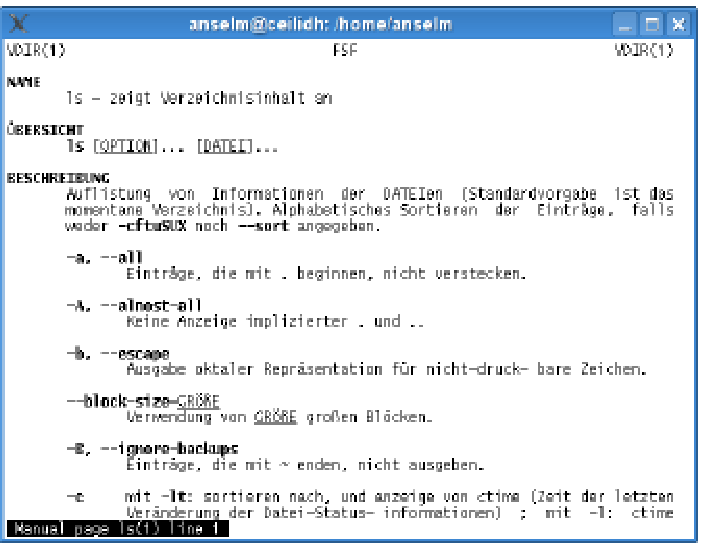
\includegraphics[width=\textwidth]{./bolum5/img1}
        \end{subfigure}%
        ~ %add desired spacing between images, e. g. ~, \quad, \qquad etc. 
          %(or a blank line to force the subfigure onto a new line)
        \begin{subfigure}[b]{0.3\textwidth}
                \centering
                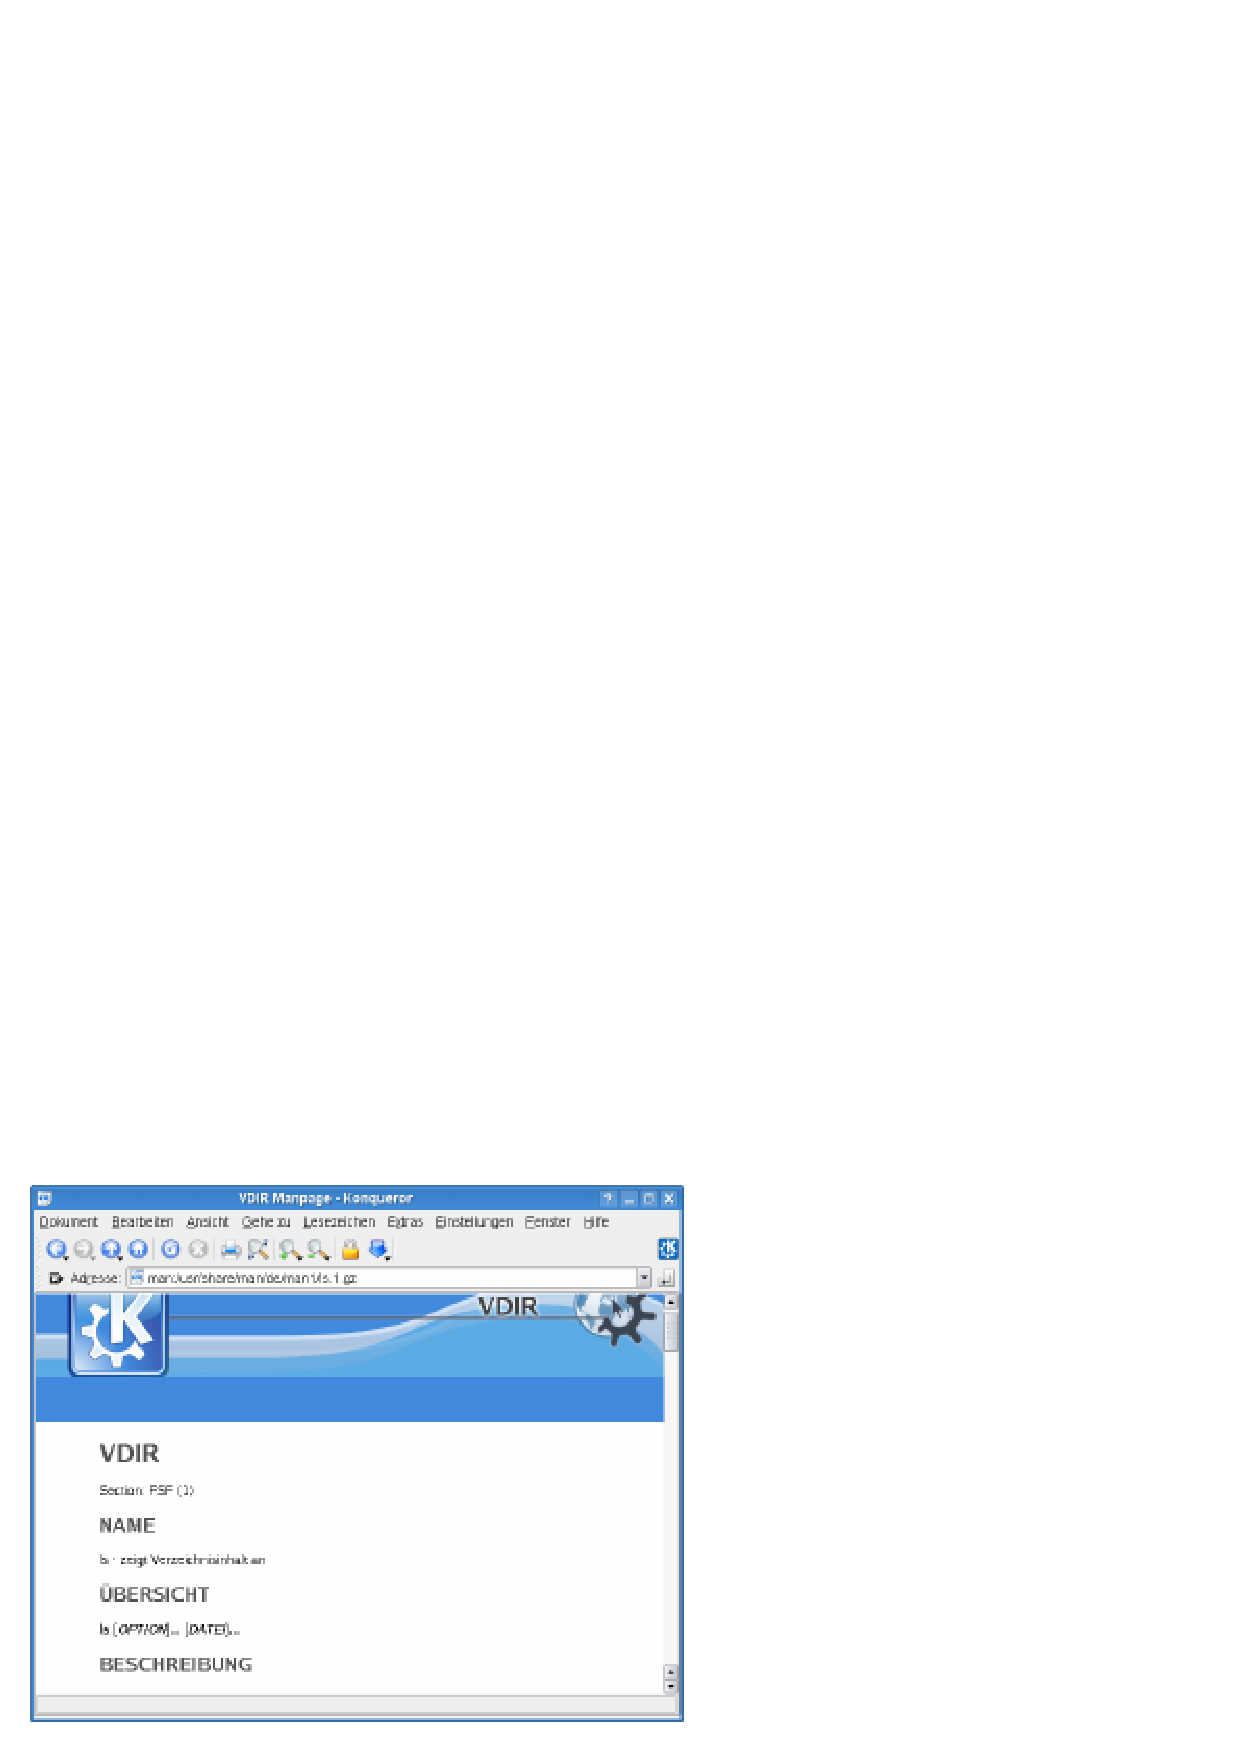
\includegraphics[width=\textwidth]{./bolum5/img2}
        \end{subfigure}
        \caption{Metin terminali (sol) ve Konqueror (sağ) içerisinde bir kılavuz sayfası }\label{fig:manpages}
\end{figure}

Amaçsızca sayısız kılavuz sayfasını aramadan önce, konu hakkında \emph{apropos} yardımıyla genel bir bilgi edinmek daha mantıklıdır. Bu komut basitçe şöyle çalıştırılır "man -k"; her ikisi de komut satırında verilen bir anahtar kelimenin "NAME" bölümlerine ilişkin tüm kılavuz sayfalarını arar. Bunun sonucunun çıktısı tüm man sayfalarını, adı veya açıklama kısmında anahtar kelimeyi de içerecek şekilde bir liste görüntüler.

Bu konuyla alakalı olan bir başka komut \emph{whatis} komutudur.Bu komut da tüm man sayfalarını arar ama yukarıda belirttiğimiz komuttan farkı \emph{whatis} aramayı anahtar kelimeye göre değil de komutun (dosya,...) \emph{adına} göre yapar. Bu istenilen komut, sistem çağrıları vs. hakkında kısaca bir açıklama görüntüler. Özellikle söz konusu man sayfasının(lar) "NAME" bölümünün ikinci  kısmını verir. \emph{whatis} ile "man -f" eşdeğerdir.
\paragraph{{\Huge{\PencilLeftDown}}Alıştırmalar}{
\begin{enumerate}
 \item \emph{ls} komutu için kılavuz sayfasını görüntüleyin. Metin tabanlı \emph{man} komutunu kullanın ve eğer mümkünse - Konqueror tarayıcısını da kullanın.
 \item Sisteminizde hangi kılavuz sayfaları (en azından "NAME" bölümlerine göre) süreçlerle iş yapar.
 \item (Ileri düzey) Kuramsal bir komutun kılavuz sayfasını yazmak için metin editörü kullanın. Önceden \emph{man}(7) kılavuz sayfasını okuyun. Kılavuz sayfasının görünürlüğünü hem ekranda ("\emph{groff -Tascii -man $<$dosya$>$ | less}" komutunu kullanarak) hem de yazılı çıktı olarak ("\emph{groff -Tps -man $<$dosya$>$ | gv -}" gibi birşey kullanın) kontrol edin.
\end{enumerate}}
\end{subsection}
\end{section}
\begin{section}{Bilgi Sayfaları}

Bazı komutlar için - genellikle karmaşık olanlar için sıradan kılavuz sayfaları yerine (ya da ilave olarak) "bilgi sayfaları" mevcuttur. Bunlar genellikle daha geniş olup World Wide Web'e benzer şekilde hiper metin prensibine göre kurulmuştur.

Bilgi sayfaları fikri GNU projesi ile birlikte ortaya çıkmıştır; o yüzden onlar en sık FSF (Özgür Yazılım Vakfı) ile  yayımlanan veya GNU projesine ait yazılımlarla gelir. Aslında "GNU sistem" için sadece bilgi belgeleri olması gerekiyordu; ancak GNU, FSF himayesinde geliştirilmeyen bir sürü yazılımları da kendi içine alır, ve GNU araçları çizgileri daha kesin olan sistemlerde kullanıldığından FSF bazı durumlarda taviz vermeye başladı.

Kılavuz sayfalarının dengi olan bilgi sayfaları "\emph{info $<$komut$>$}" komutu (bilgi programını içeren paket açıkça kurulmuş olması gerekebilir) kullanılarak görüntülenir. Ayrıca, bilgi sayfaları \emph{emacs} editöründe veya KDE web tarayıcısı Konqueror'da URL'ler yardımıyla "\emph{info:/$<$komut$>$}" görüntülenebilir.

Bilgi sayfalarının bir avantajı, kılavuz sayfaları gibi kaynak formatında yazılmış olmalarıdır. Bilgi sayfaları PDF ve PostScript formatında yazdırılabilir veya ekranda işlenebilir. \emph{groff} yerine, \TeX{} dizgi programı çıktı işlemi için hazırlanabilir.

\paragraph{{\Huge{\PencilLeftDown}}Alıştırmalar}{
\begin{enumerate}
 \item \emph{ls} programı için bilgi sayfasına bakın. Metin tabanlı bilgi tarayıcısı ve, varsa, Konqueror tarayıcısını deneyin.
 \item Bilgi sayfaları günümüzde HTML dosyalarının World Wide Web'de olduğu gibi hiper metnin ilkel formunu kullanır. Bilgi sayfaları neden HTML ile yazılmamıştır?
\end{enumerate}}
\end{section}
\begin{section}{NASIL Belgeleri}

Kılavuz ile bilgi sayfaları arasındaki ortak problem şudur: Kullanıcılar kullanacakları programın adını bilmek zorundadırlar. Hatta \emph{apropos} ile arama yapmak şans oyunu gibi birşeydir. Ayrıca, her problem tek bir komut kullanılarak çözülemez. Bu nedenle bunlar "komut odaklı" belgeler yerine genellikle "problem odaklı" olarak adlandırılır. Nasıl Yapılır kısmı bunlara çözüm üretmek için tasarlandı.

Nasıl Belgeleri kendilerini tek bir komutla  kısıtlamayan geniş kapsamlı belgelerdir, ama sorunların çözümü için tam yaklaşımları açıklamaya çalışırlar. Örneğin, DSL yoluyla Linux sisteminin internete nasıl bağlanacağını detaylı olarak açıklayan "DSL Nasıl" belgesi vardır, ya da Linux için astronomi yazılımını tartışan "Astronomi NASIL" vardır. Nasıl Yapılır kısımlarının birçoğu İnglizce aslını genellikle geriden takip etse de bunlar başka dillerde de mevcuttur.

Çoğu Linux dağıtımı Nasıl Belgelerinin (veya büyük bir alt kümesinin) yerel olarak kurulu olmasını sağlar. Bunlar dağıtıma özel dizinlerin altında bulunurlar. /usr/share/doc/howto SUSE dağıtımları için, /usr/share/HOWTO Debian GNU/Linux içindir. Tipik olarak düz metin veya HTML dosyaları içerir. Nasıl Yapılır'ların geçerli tüm sürümleri ve diğer PostScript veya PDF biçimindekilerinin hepsi internet üzerinde "Linux Belgelendirme Projesi" (http://www.tldp.org) altında bulunabilir. Bu adres ayrıca diğer Linux belgelerini de sunar.
\end{section}
\begin{section}{Ek Bilgi Kaynakları}

Neredeyse her kurulu olan yazılım için ilave belgeleri veya örnek dosyaları /usr/share/doc ya da /usr/share/doc/packages (kullandığınız dağıtıma bağlı olarak değişir) altında bulunur. Çoğu GUI uygulamaları (KDE veya GNOME paketlerindeki gibi) "yardım" menüsü sunar. Üstelik birçok dağıtım uzmanlaştırılmış "yardım merkezleri" sunar. Sistem üzerindeki çoğu belgelere uygun erişimi sağlar.

Yerel sistemden bağımsız olarak WWW ve USENET arşivlerinin de arasında bulunduğu, pek çok belge Internet ortamında bulunmaktadır. 

Linux için daha ilgi çekici sitelerden bazıları:
\paragraph{http://www.tldp.org/}{“Linux Belgelendirme Projesi”, kılavuz sayfaları ve Nasıl Yapılır'dan sorumlu (diğer şeylerin yanı sıra).}
\paragraph{http://www.linux.org/}{Linux meraklıları için genel portal.}
\paragraph{http://www.linuxwiki.de/}{Linux ile ilgili her şey için serbest biçimli metin bilgi veritabanı (Almanca)}
\paragraph{http://lwn.net/}{Haftalık Linux Haberleri - her türlü Linux haberleri için belki de en iyi web sitesi. Yeni gelişmeler, ürünler, güvenlik açıkları, basındaki Linux savunuculuğu vs. ayrıca her persembe günü geçmiş haftaların araştırmalarının yer aldığı çevrimiçi dergi de bulunur. Günlük haberlere ücretsiz olarak ulaşılabilir iken haftalık yayınlamalara belli bir ücret ödenmesi gerekiyor (aylık 5\$'dan başlayan fiyatlarla). İlk çıktığı haftadan sonra o yayınları ücretsiz olarak erişilebilir hale getiriyorlar.}
\paragraph{http://freecode.com/}{Bu site yeni (genel olarak serbest) çıkan yazılım paketlerini tanıtır. Buna ek olarak ilginç projeler veya yazılım paketleri için sorguları sağlayan bir veritabanı var}
\paragraph{http://www.linux-knowledge-portal.de/}{LWN ve Freshmeat dahil diğer Linux sitelerinden haber başlıklarını toplar.}

Eğer Internette veya Usenet arşivlerinde bulmadıysanız aradığınızı, sorunuza cevabı  posta listelerinde ya da Usenet gruplarında soru sormak her zaman mümkündür. Bu forumlardaki çoğu kullanıcıların daha önce cevaplanmış ya da belgelendirmede veya "SSS" (Sıkça Sorulan Sorula) kısmında olan birşeyi sormanıza kötü tepki verebileceklerini unutmayın. Probleminizin detaylı açıklamasını hazırlayın, kayıt dosyalarından ilgili ayrıntıları verin çünkü karmaşık problemleri sizde olduğu gibi uzak mesafeden çözmek zordur (karmaşık olmayan problemleri kendinizin çözebiliyor olmanız lazım).

Haber arşivlerini \emph{http://groups.google.com/} (eskiden DejaNews) adresinde bulabilirsiniz.

Linux için ilgi çekici \emph{haber grupları} İngilizce için \emph{comp.os.linux.*} veya Almanca için \emph{de.comp.os.linux.*} hiyerarşilerinde bulunabilir. Birçok Unix grupları Linux konuları için uygundur; kabukla ilgili soruların kabuk programlama için ayrılan grupta sorulması gerekir, Linux grubunda değil, çünkü kabuklar genellikle Linux'a özgü değildir.

Linux tabanlı posta listelerini örneğin, \emph{majordomo@vger.kernel.org} adresinde bulabilirsiniz. LIST denilen listeye katılmak için önce "subscribe LIST" adresine e-posta atmanız gerekir. Sistemde mevcut yorumlanmış tüm posta listeleri \emph{http://vger.kernel.org/vger-lists.html} adresinde bulabilirsiniz.

Görünüşte anlaşılmayan problemleri çözmenin yolu hata mesajının Google'da aratmaktır(ya da güvendiğiniz baska bir arama motoru). Eğer faydalı bir sonuç alamazsanız, arama yaptığınız sorguda sadece size özel duruma bağlı kısımları kaldırın (mesela alan adları gibi). Google'da aramanın avantajı sadece ortak web sayfalarını indekslemek değil bunun yanında posta liste arsivlerini de indeksler. O yüzden sizin gibi sorunu yaşayan bir başka birilerinin bulunması da olası bir durum.

Açık kaynak kodlu yazılımların büyük miktarda belgelendirmelerinin olması tek büyük faydaları değildir ayrıca çoğu belgelendirmenin de en az yazılımının kendisi gibi kısıtlı olmasıdır. Bu, yazılım geliştiricileri ve belge yazarları arasındaki işbirliğini kolaylaştırır ve belgelerin diğer dillere çevrilmesi daha kolaydır. Aslında, programcı olmayanlar için özgür yazılım projelerine destek verebilmeleri için bol fırsat bulunmaktadır, örn. iyi belgelemeler yazmak. Özgür yazılım faaliyet alanında programcılara verilen saygıyı belge yazarlarına da vermeye çalışılmalı. Bu durum kaymasının başlamış olması henüz tamamlandığı anlamına gelmemektedir.
\end{section}
\paragraph{Bu Bölümdeki Komutlar}{
\begin{itemize}
\item[apropos] NAME bölümünde verilen anahtar kelimeyi içeren tüm kılavuz sayfalarını görüntüler
\item[groff] Gelişmiş dizgi programı
\item[help]	\emph{bash} komutları çevrim için yardımı görüntüler
\item[info] Karakter tabanlı terminalde GNU Bilgi sayfalarını görüntüler
\item[less] Metinleri sayfa sayfa (kılavuz sayfaları gibi) görüntüler
\item[man] Sistem kılavuz sayfalarını görüntüler
\item[manpath] Sistem kılavuz sayfalarının aranacağı yolu belirler
\item[whatis] Açıklamasında verilen belirli bir anahtar kelime ile kılavuz sayfalarını bulur
\end{itemize}
}
\paragraph{Özet}{
\begin{itemize}
\item "\emph{help $<$komut$>$}" dahili bash komutlarını açıklar. Birçok harici komut \emph{--help} seçeneğini destekler.
\item Çoğu program kılavuz sayfalarıyla gelir. Bunlar \emph{man} komutuyla incelenebilir. \emph{apropos} verilen anahtar kelimelere göre tüm kılavuz sayfalarını arar, \emph{whatis} kılavuz sayfa isimlerine bakar.
\item Bazı programlar için bilgi sayfaları kılavuz sayfalarına bir alternatiftir.
\item Nasıl Yapılır belgeleri problem tabanlı bir belgeleme olustururlar.
\item World Wide Web ve USENET dünyasında Linux ile ilgili çok sayıda ilginç kaynaklar var.
\end{itemize}}
\chapter{Dosyalar: Bakım ve Besleme}
\label{chap:bolum6}
\paragraph{Amaçlar}
\begin{itemize}
 \item Linux kurallarıyla birlikte dosya ve dizin isimleriyle uğraşmaya alışmak
 \item Dosya ve dizinlerle çalışmada önemli komutları bilmek
 \item Kabuk dosya adı arama şablonlarını kullanabilmek
 \end{itemize}
 
\paragraph{Önceden Bilinmesi Gerekenler}
\begin{itemize}
 \item Kabuk kullanımı
 \item Metin editörü kullanımı
 \end{itemize}

\begin{section}{Dosya ve Yol İsimleri}
\begin{subsection}{Dosya İsimleri}

Linux gibi işletim sisteminin en önemli hizmetlerinden birisi de, veriyi sabit disk veya USB sürücüler gibi kalıcı hafızaya depolamak ve sonrasında onları kullanmaktır. Bu işi insan açısından katlanılabilir kılmak için, benzer veriler cihaz üzerinde "dosyalar" altında toplanır.

Eğer bu bile sizin için önemsiz gözüküyorsa, bu anlatılanların size hiçbir getirisi yoktur. Eskiden bazı işletim sistemleri, bir verinin bilgisini almak için disk üzerindeki iz sayıları gibi ayrıntıları belirtmeyi zorunlu kılıyordu. 

Bu yüzden, size dosyalarla nasıl uğraşılacağını anlatmaktan önce, Linux'un dosyaları nasıl isimlendirdiğini açıklamalıyız.

Linux dosya isimlerinde, aslında bilgisayarınızın gösterebileceği her karakteri (hatta daha fazlasını) kullanmanıza olanak tanır. Ancak, karakterlerden bazılarının özel anlam içerdiğinden beri, dosya isimlerinde bu karakterleri kullanmanızı tavsiye ederiz. Yalnızca iki karakterin kullanılamaz: bölü ("/") işareti ve 0 byte (ASCII değeri 0 olan karakter). Boşluk, inceltme işareti ya da dolar işaretleri gibi karakterler serbestçe kullanılabilir, fakat kabuk tarafından yanlış yorumlanmakyan kaçınmak için komut satırında "$\backslash$" veya tırnak işaretleri kullanılarak bu karakterlerden kaçılır.

Acemilerin kolayca tuzağa düşeceği olay ise, Linux'un dosya isimlerinde büyük/küçük harfleri ayırt edebilmesidir. Büyük ve küçük harfli dosyaların ayrı gösterildiği fakat aynı davranıldığı Windows işletim sisteminin tersine Linux \emph{x-files} ve \emph{X-Files} dosya isimlerini iki farklı dosya olarak ele alır.

Limitlerin "dosya sistemine" bağlı olduğundan beri, Linux altında byte'lar halinde düzenlenen dosya adları "çok uzun", belli bir üst limit yoktur, olabilir( Linux'ta  bu düzenlemeyle ilgili birçok yöntem vardır). Normal sınır 255 karakterdir, fakat 3 satırdan daha fazla uzunlukta dosya isimleri standart metin terminalinde size bir karmaşıklık oluşturmamalıdır.
	
DOS ve Windows bilgisayarlardan başka bir fark da Linux, dosyanın tipini belirlemek için sonekleri kullanmaz. Bu yüzden, dosya ismindeki nokta tamamen sıradan bir karakterdir. Bir metin dosyasını \emph{mumble.txt} olarak kaydetmede serbestsiniz, fakat prensip olarak sadece \emph{mumble} kelimesi de  kabul edilebilir. Bu kullanım tabi ki sizin tamamen uzantı ile adlandırmanızı engellememelidir, sonuçta bu kullanım dosya içeriğini tanımlamanızda kolaylık sağlar.
	
Bazı programlar girdi dosyalarında özel uzantı kullanmayı zorunlu kılar. Örneğin C derleyicisi olan \emph{gcc}, "\emph{.c}" ile biten C kaynak kodu, "\emph{.s}" ile biten makine dili kaynak kodu ve "\emph{.o}" ile biten ön derlenmiş nesne dosyaları isimlerini dikkate alır.
	
Dosya isimlendirmede özgürce inceltme işareti ve diğer özel karakterleri kullanabilirsiniz. Yine de, eğer dosyalar diğer sistemlerde kullanılacaksa özel karakterleri kullanımından kaçmak en iyisidir, çünkü diğerlerinde dosyaların aynı isimle gösterileceğinin bir garantisi yoktur.
	
Özel karakterlerin ne olduğu sizin yerel ayarlarınıza bağlıdır, çünkü ASCII karakter setini (Çoğunlukla içinde İngilizce dili, rakamlar ve yaygın özel karakterlerin bulunduğu 128 karakter) aşan karakterlerin temsili için genel bir standart yoktur. Çokça kullanılan kodlamalara örnek olarak ISO 8859-1 ve ISO 8859-15 (sırasıyla ISO-Latin-1 ve ISO-Latin-9 olarak bilinir) bununla birlikte gelişigüzel ve çok doğru olmayarak adına "Unicode" denilen genellikle "UTF-8" karakter seti ile kodlanan ISO 10646. Y kodlaması sistemde yürürlükte iken dizine baktığınız zaman X kodlamasıyla oluşturduğunuz dosyalar tamamen farklı gözükebilir. Bu konuların üzerinde çok durursanız, size tüm konu hiçbir şey gibi gelir.
	
Bazen kendinizi yanlış karakter setiyle kodlanmış bir yığın dosya ile uğraşıyor olarak bulabilirsiniz. Çeşitli karakter setleri arasında dönüşüm yapabilen \emph{convmv} programı bu konuda size yardım edebilir. (Çoğu dağıtımın standart kurulumunun bir parçası olmadığından, muhtemelen kendiniz yüklemeniz gerekecektir.) Ancak, bunu tüm bölümü bitirdiğimiz zaman yapmanız daha uygun olur, çünkü daha normal \emph{mv}'den bahsetmedik bile\ldots
	
Aşağıdaki tüm karakterleri dosya isimlendirmelerinde özgürce kullanabilirsiniz:
\begin{verbatim}
 ABCDEFGHIJKLMNOPQRSTUVWXYZ
 abcdefghijklmnopqrstuvwxyz
 0123456789+-._
\end{verbatim}

Ancak aşağıdaki ipuçlarına dikkat etmelisiniz:
\begin{itemize}
\item Linux ve daha eski Unix sistemleri arasında dosya taşımalarını mümkün kılmak için dosya isimleri en fazla 14 karakter olmalıdır. (Bu kurala uymak gerçekten önemlidir.)
\item Dosya isimleri her zaman harf veya rakamlardan biriyle başlamalıdır; diğer 4 karakterleri sadece dosya içerisinde sorunsuzca kullanabilirsiniz.
\end{itemize}

Bu kuralları anlamanın en kolayı birkaç örneği incelemektir. Uygun dosya isimlerine örnek olarak
\begin{verbatim}
X-files
foo.txt.bak
50.something
7_of_9
\end{verbatim}
verilebilir. Buna karşılık aşağıdaki kullanımlar problem oluşturabilir (muhtemelen):
\begin{verbatim}
-10F 		‘‘- ’’ ile başlıyor, özel karakter var
.profile 					Gizli dosya olacaktır
3/4-metre 				Kural dışı karakter içerir
Smörrebröd 					İnceltme işareti içerir
\end{verbatim}

Diğer bir tuhaf özellik de, dosya isimlerinin nokta (".") ile başlaması bazı yerlerde dosyanın gözden kaçmasına neden olacak, örneğin dizin içerisindeki dosyaların listelendiği zaman, bu tür dosya isimleri "gizli" gibi düşünülür. Bu özellik genellikle programların içerik ayarlarında ve dizin listelemelerde çok daha önemli dosyaların kullanıcının kafasını karıştırmamak amacıyla kullanılır.

DOS ve Windows uzmanları için: Bu sistemler dosyanın isminden bağımsız olarak "dosya özniteliklerinin" "gizli" olması ile izin verir. Linux ve Unix böylesi bir işi desteklemez.
\end{subsection}
\begin{subsection}{Dizinler}

Potansiyel olarak birçok kullanıcı aynı Linux sisteminde alıştığından, tüm dosya isimlerinin sadece bir tane olması problem teşkil edebilirdi. Sue kullanıcısı halihazırda aynı isimde bir dosyaya sahip olduğu için Joe kullanıcısının \emph{letter.txt} isimli bir dosya oluşturmasını oldukça güç hale sokar. Ayrıca Joe'nun, Sue'nun tüm dosyalarını okuyamamasını garanti eden uygun bir yol bulunması gerekir.

	Bu nedenle, Linux dosyaları gruplamak için aşamalı  "dizin" fikrine destek verir. Aynı dizindeki dosyalar dışında, dosya isimlerinin  tüm sistemde eşsiz olması gerekmez. Özellikle bu, sistemin Joe ve Sue için farklı dizinler atayabilmesini, ve her birinin kendi dosyaları hakkında diğerlerininkilerin isimlerini dert etmeden çağırabilmeleri anlamına gelir.
	
	Ek olarak, Joe'ya Sue'nun \emph{dizinine} (veya tam tersi) erişmesini yasaklayabiliriz ve dizin içerisindeki kişisel dosyalar hakkında endişelenmemize gerek kalmaz.
	
	Linux'ta dizinler basit dosyalar olsa da, "düz" dosyalara erişmek için kullandığınız yöntemler ile onlara erişemeyebilirsiniz. Ancak, daha önce bahsettiğimiz dosya isimleri kurallarını(önceki bölüme bakınız) dizin isimlendirmelerinde de göz önünde bulundurmanız gerekir. Sadece bölü ("/") karakterinin, dizin isimlerinden dosya isimlerini ve dizinleri birbirlerinden ayrımak için kullanıldığını bilmeniz yeterlidir. Örnek olarak: \emph{joe/letter.txt}, \emph{joe} dizinindeki \emph{letter.txt} dosyasıdır.
	
	Dizinler ağaç-benzeri (yaratıcı bir şekilde "dizin ağacı" denen) yapı ile tasvir edilen diğer dizinleri içerebilir (bu "aşamalı" teriminden daha önce de bahsetmiştik). Bir Linux sistemi, ağacın kökleri gibi bir yapıda olan "kök dizini" denilen özel bir dizin içerir. "/"(bölü) ile ifade edilir.
	
	İsminin aksine, kök dizininin, sistem yöneticisi anlamına gelen \emph{root} ile alakası yoktur. Sadece isimleri benzerdir.
	
	Burada bölünün çift görevi vardır, hem kök dizininin adıdır, hem de dizin isimleri arasında ayraç görevi üstlenir. Bu konuya birazdan geri döneceğiz.
	
	Yaygın Linux dağıtımlarındaki temel yükleme, genellikle tek bir dosya hiyerarşisinde bulunan ve bunun çokça belirli düzene göre yapılandırılmış olduğu onbinlerce dosyayı içerir. Bu dosya hiyerarşisine Bölüm ~\ref{chap:bolum10}'da daha çok yer vereceğiz.
\end{subsection}
\begin{subsection}{Mutlak ve Göreceli Yol İsimleri}

Linux sistemindeki her dosya, kök dizini tarafından başlayan, bir dosyaya (dosyanın kendisine) ulaşıncaya kadar devam eden tüm dizinlerin adının geçtiği ve sonunda dosyanın kendisinin bulunduğu dosya isimleriyle tasvir edilir. Örneğin, \emph{/home/joe/letter.txt} ismi, \emph{joe} dizini altında bulunan, \emph{home} dizini içerisinde konumlanan, daha sonra da evebeyn olan kök dizininin yer aldığı \emph{letter.txt} dosyasına karşılık gelir. Kök dizini ile başlayan isimlere "mutlak yol ismi" adı verilir. İsimler dizin ağacı içerisinde dizin ve dosya isimleri barındıran "yol" vasıtasıyla tanımlandığından "yol isimleri" lafını kullanırız.

	Linux sisteminde her sürecin bir "mevcut dizini" (genellikle "çalışma dizini" diye adlandırılır) vardır. Dosya isimleri bu dizinin içerisinde aranır; \emph{letter.txt} "mevcut dizin içerisindeki letter.txt" için, \emph{sue/letter.txt} "sue dizini içerisindeki, letter.txt" için bir kısaltmadır. Mevcut dizinden başlayan bu tarz isimlere "göreceli yol isimleri" adı verilir.
	
	Göreceli yol isimlerinin mutlak olduğunu söylemek önemsizdir: Mutlak dosya yolu bir "/" ile başlar; diğer hepsi görecelidir.
	
Mevcut dizin evebeyn ve çocuk süreçler arasındaki "miras" olarak aktarılır. Yani kabuktan yeni bir kabuk başlattığınızda(veya başka bir program), bu yeni kabuk, sizin başlatmak için kullandığınız kabuk dizini ile aynı mevcut yolu kullanır. Yeni kabuğunuzda diğer dizine \emph{cd} komutunu kullanarak geçebilirsiniz, fakat eski kabuğun mevcut dizini değişmez. Eğer yeni kabuktan ayrılırsanız, eski kabuğun mevcut dizinine (değişmemiş dizine) geri dönersiniz. 
	
	Göreli yol isimlerinde(hatta mutlak olanlarda bile) iki kullanışlı kestirme vardır: ".." ismi her zaman dizin ağacında bir bilinmeyen olan mevcut dizinin üst dizinini işaret eder. Örneğin, \emph{/home/joe}, \emph{/home} durumudur. Bu sıklıkla mutlak yol ismine başvurmak zorunda kalmadan, mevcut dizinden, dizin ağacı gibi gösterilen "yan dal"'a ayrılmak için kullanışlı bir yoldur. Farzedelim ki \emph{/home/joe} dizininin \emph{letters} ve \emph{novels} isminde altdizinleri olsun. \emph{letters} sizin mevcut dizininiz gibi olsun, \emph{novels} dizininin içerisinde \emph{ivanhoe.txt} dosyasına kaba bir şekilde mutlak yol ismi olan \emph{/home/joe/novels/ivanhoe.txt}'yi kullanmaksızın \emph{../novels/ivanhoe.txt} şeklinde göreceli yol ismi belirterek referans belirtebilirsiniz.
	
İkinci kestirme ise size açıkça bir anlam ifade etmiyor gibi gelebilir: "." ismi dizin içerisinde bulunur ve her zaman dizinin kendisini ifade eder. Neden zaten içinde bulunduğumuz dizine işaret eden böyle bir metoda ihtiyacımızın olduğunun doğrudan bir cevabı yoktur, fakat  tabi ki bu durumların bize kattığı kullanışlı beceriler vardır. Örneğin, belki biliyorsunuzdur (ya da Bölüm ~\ref{chap:bolum9}'a bakınız) kabuğun harici komutlar için program dosyalarını ararken kullandığı çevresel dizin değişkeni olan \emph{PATH} vardır. Diyelim ki bir yazılım geliştiricisisiniz, bir program çalıştırmak istiyorsunuz, \emph{prog} olarak isimlendirdiğimiz, (a) mevcut dizininiz içerisindeki bulunan ve (b) \emph{PATH} içerisinde yer almayan (Güvenlik nedenleri için her zaman iyi bir fikirdir) dizininiz içerisindeki \emph{prog}'u çalıştıralım, halâ kabuğunuzdayken
\begin{verbatim}
 $ ./prog
\end{verbatim} 
diyerek dosyanızı, mutlak yol ismini vermek zorunda kalmadan program olarak başlatabilirsiniz.

Linux kullanıcısı olarak sisteme girdiğinizden hemen sonra "ev dizinine" ulaşırsınız. Sistem yöneticisi sizin hesabınızı oluşturduğunda bu dizinin ismine karar verir, fakat genellikle kullanıcı isminizle aynı olur ve /home dizini altında yer alır, \emph{joe} kullanıcısı için atanan \emph{/home/joe} gibi.

\end{subsection}
\end{section}

\begin{section}{Dizin Komutları}
\begin{subsection}{Mevcut Dizin: cd \& Co.}

Mevcut dizini değiştirmek için cd kabuk komutunu kullanabilirsiniz: Basitçe parametre olarak arzu edilen dizin ismi verilir:
\begin{verbatim}
$ cd letters 	       letters dizinine değiştirir
$ cd .. 			   Bir üstteki dizine değiştirir
\end{verbatim}

Eğer parametresiz kullanacak olursanız ev dizininize erişirsiniz:

\begin{verbatim}
$ cd
$ pwd
/home/joe
\end{verbatim}

Mevcut dizinin mutlak yolunun çıktısını almak için pwd ("print working directory") komutunu kullanabilirsiniz.

Ayrıca mevcut dizininizi büyük olasılıkla kendi istemcinizin bir kısmı olarak görebilirsiniz. Sistem ayarlarınıza bağlı olarak

\begin{verbatim}
joe@red:~/letters> _
\end{verbatim}

gibi bir satırla karşılaşabilirsiniz. $\sim$/letters /home/joe/letters'a kısaltmadır; tilda ("$\sim$") ise mevcut kullanıcı ev dizininizi gösterir. "cd -" komutu cd komutu ile son kullanılmış dizine tekrar geri dönmeyi sağlar. Bu kullanışlı komut iki dizin arasında peş peşe geçiş yapmayı sağlar.

\paragraph{{\Huge{\PencilLeftDown}}Alıştırmalar}{
\begin{enumerate}
 \item Kabukta cd dahili mi, harici mi komuttur? Neden?
 \item Kabuk kılavuz dosyasında pushd, popd, dirs komutlarını okuyunuz. Bu komutların tasvir edildiği gibi çalıştığına kendinizi ikna ediniz.
\end{enumerate}}

\paragraph{}{
\begin {table}[H]
\caption {ls'deki bazı dosya gösterimleri} \label{tab:tablo61} 
\begin{tabular}{l c c c}
\hline
Dosya Tipi & Renk & Sonek (ls -F) & Harf türü (ls -l) \\
\hline
düz metin 	&	siyah & none & - \\
çalıştırılabilir dosya 	&	yeşil & * & - \\
dizin 	&	mavi & / & d \\
link 	&	cyan & @ & l \\
\hline
\end{tabular}
\end {table}
}

\paragraph{}{
\begin {table}[H]
\caption {Bazı ls parametreleri} \label{tab:tablo62} 
\begin{tabular}{l l}
\hline
Parametre & Sonuç \\
\hline
-a veya --all 	&	Aynı zamanda gizli dosyaları da görüntüler \\
-i veya --inode 	&	Eşsiz dosya numarasını görüntüler (inode number) \\
-l veya --format=long 	&	Ekstra bilgi görüntüler \\
-o veya --no-color 	&	Çıktı renk-kodlamasını atlar \\
-p veya -F 	&	Eklenen özel karakterle dosya türünü işaretler \\
-r veya --reverse 	&	Sıralamayı ters yapar \\
-R veya --recursive 	&	Alt dizinlerle birlikte rekürsif olarak listeler (DOS: DIR/S) \\
-S veya --sort=size 	&	Boyuta göre sıralar (büyükten küçüğe doğru) \\
-t veya --sort=time 	&	Değiştirilme tarihine göre sıralar (yeniden eskiye doğru) \\
-X veya --sort=extension 	&	Dosya uzantısına göre sıralar (“dosya türüne” göre) \\
\hline
\end{tabular}
\end {table}
}
\end{subsection}
\begin{subsection}{Dosya ve Dizinleri listeleme --ls}

Dizin ağacı etrafında yolunuzu bulmak için hangi dosya ve dizinlerin mevcut dizin içerisinde olduğunu bilmeniz gerekir. ls("list") komutu tam da bu iş için vardır.

Parametresiz kullanımda çıktı olarak dosyaların isme göre sıralandığı bir çeşit tablo görünümlü bir yapı elde edilir. Renkli ekranların günümüzde standart haline gelmesiyle, dosya isimleri ve türlerinin farklı renklerde görüntülenmesi genelek haline geldi (Daha dosya tipleri hakkında konuşmadık; bu konuya Bölüm ~\ref{chap:bolum10}'da değineceğiz).
	
Neyse ki, günümüzde birçok dağıtım renkli kullanımı bünyesinde barındırıyor. Tablo ~\ref{tab:tablo61}'de en yaygın gösterimler vardır.

Siyah-Beyaz ekranlarda, ki hala günümüzde var, -F veya -p parametreleri önerilir. Bunlar dosya türleri ile ilişkili dosya isimlerine özel karakter eklerler. Bu karakterlerin bazılarına Tablo ~\ref{tab:tablo61}'de değinmiştik.
	
Gizli dosyaları (nokta ile başlayan isimlileri) -a ("all") parametresiyle görüntüleyebilirsiniz. Bir başka kullanışlı seçenek ise -l'dir(büyük harf olarak "L", "long"(uzun) anlamı taşır, "1" rakamı değildir). Bu sadece dosya isimlerini sıralamakla kalmaz ayrıca her dosya için ek bilgi de içerir.
	
Bazı Linux dağıtımlarında önceden ayarlanmış bazı yardımcı parametrelerin kombinasyonu olan kısaltmalar vardır; SUSE dağıtımlarında, örneğin sadece basit bir l kullanımı "ls -alF"'nin kısaltmasıdır. "ll" ve "la" ls'nin farklılaşmış bazı kısaltmalarıdır.
	
Aşağıdaki örnekte ls'nin -l'li ve -l'siz kullanımı vardır:
\begin{verbatim}
$ ls
file.txt
file2.dat
$ ls -l
-rw-r--r-- 1 joe users 4711 Oct 4 11:11 file.txt
-rw-r--r-- 1 joe users 333 Oct 2 13:21 file2.dat
\end{verbatim}

İlk durumda, bütün gizli olmayan dosyalar listelendi; ikinci durumda ise ekstra bilgi eklendi.

	Uzun formatın farklı parçalarının anlamları vardır: İlk karakter dosya türünü verir (Bölüm ~\ref{chap:bolum10}'a bakınız); sade dosyalar "-", dizinler "d" şeklinde vb.(Tablo ~\ref{tab:tablo61}'deki "karakter türleri").
	
	Sonraki 9 karakter erişim izinlerini gösterir. Sonraki dosyanın adedini, dosyanın sahibini(joe), ve dosyanın grubunu(users) gösterir. Byte olarak dosyanın boyutundan sonra, dosyanın içerdiği son değiştirilme bilgisini tarih ve saat olarak görebilirsiniz. Ve tabi ki dosyanın adı da görüntülenir.
	
	Kullandığınız dile bağlı olarak özellikle tarih ve saat sütunları örmeklerimizden(asgari dil ortamı "C" kullanarak oluşturduğumuz) tamamen farklı görünebilir. Bu genellikle interaktif kullanımda sorun çıkarmaz, fakat eğer kabuk betiğinizin bir bölümünde "ls -l"'nin çıktısını almaya çalışıyorsanız büyük bir sıkıntı ortaya çıkabilir. (Gelişmiş Linux kılavuzunu çalışmaktan önce, kabuk betiklerinde ön tanımlanmış dil çevreselini kullanmanızı öneririz.)
	
	Eğer dizin için ekstra bilgi görmek isterseniz(/tmp dizini gibi), "ls -l /tmp"'nin size gerçekten bir yardımı dokunmaz, çünkü ls /tmp içerisindeki tüm dosyaların verisini listeleyecektir. -d parametresi kullanarak /tmp'nin kendisinin bilgisini elde edebilirsiniz.
	
ls burada bahsedilenlerden çok daha fazlasına destek verir; önemli olanlarından bir kaçı Tablo ~\ref{tab:tablo62}'de gösterilmişti.

Linux Essentials ve LPI-101 gibi LPI sınavlarında, kimse sizden ls'nin tüm 57 tane parametresini bilmenizi beklemez. Ancak en önemli yarım düzine kadarını—yaklaşık Tablo ~\ref{tab:tablo62} içeriğindeki kadarını— ezberlemek isteyebilirsiniz.
\paragraph{{\Huge{\PencilLeftDown}}Alıştırmalar}{
\begin{enumerate}
 \item /boot dizinini hangi dosyaları içerir? Alt dizinleri var mıdır? Varsa hangileridir?
 \item Dosya ismini parametre olarak alan ls ile dizin ismini parametre olarak alan ls arasındaki fark nedir?
 \item Eğer dizin adı programda geçiyorsa, dizindeki dosyaların bilgisini görüntülemektense ls'ye sadece dizinleri göstermesi için hangi parametre ile çalıştırırız? (İpucu:Belgeye bakınız.)
\end{enumerate}}
\end{subsection}
\begin{subsection}{Dizin Oluşturma ve Silme: mkdir ve rmdir}

Dosyalarınızı düzenli bir şekilde tutmak istediğinizde yeni bir dizinler oluşturmak iyi bir fikirdir. Dosyalarınızı ilişkili konuya göre (Örnek olarak) bu "klasörler" altında toplayabilirsiniz. Tabi ki ileri bir yapılandırma için, ek dizinlerle çalışarak dosyalarınızı bu dizinler altında tutabilirsiniz - hevesinizi, keyfi engeller tarafında sınırlamayınız.

mkdir komutu yeni dizinler oluşturmak için yegane komuttur. Argüman olarak bir veya daha çok dizin ismi alır, aksi halde yeni dizin oluşturmak yerine sadece bir hata mesajı alırsınız. İç içe dizinleri tek adımda oluşturabilmek için -p parametresini kullanabilirsiniz, aksi halde komut, oluşturduğunuz yoldaki dizinlerin hepsini varmış gibi farzedecektir. Örneğin:
\begin{verbatim}
$ mkdir pictures/holiday
mkdir: cannot create directory `pictures/holiday': \\
No such file or directory
$ mkdir -p pictures/holiday
$ cd pictures
$ ls -F
holiday/
\end{verbatim}
\end{subsection}
\end{section}

\begin{section}{Dosya Arama Şablonları}
\label{sec:bolum63}
\begin{subsection}{Basit Arama Şablonları}

Sık sık aynı süre içerisinde birçok dosya için bir komut uygulamak isteyebilirsiniz. Örneğin, eğer "p" ile başlayıp ".c" ile biten tüm dosyaları prog1 dizininden prog2 dizinine kopyalamak istediğinizde, her dosyanın ismini açık bir şekilde yazmak oldukça sıkıcı olabilir— eğer en azından birçok dosya ile uğraşıyorsanız! Kabuk arama şablonları kullanarak bu iş çok rahat bir şekilde yapılır.

Kabuk komut satırında belirlediğiniz bir kelimeyi yıldız ile kullanarak bunu sağlayabilirsiniz. Örneğin
\begin{verbatim}
prog1/p*.c
\end{verbatim}
Kabuk bu parametreyi, dosya isimlerinin "eşleşme" parametresine göre sıralandığı liste ile mevcut olan asıl programda başlatır. "Eşleşme", asıl dosya adında, yıldızlı keyfi karakterlerin istenen uzunlukta sıralanmasına denir. Örneğin
\begin{verbatim}
prog1/p1.c
prog1/polly.c
prog1/pop-rock.c
prog1/p.c
\end{verbatim}
yukarıdaki isimler uygundur (örnekteki son ismin özelliği için kısa not — "istenen uzunluk", "sıfır uzunluğu" içerebilir!). Yıldız ile eşleştirilemeyecek bir karakter sizce ne olabilir?—taksim işareti; genellikle arama şablonundaki yıldız karakterini bulunduğunuz dizin ile sınırlamak daha iyidir.

echo ile kolay bir şekilde bu arama şablonlarını test edebilirsiniz.
\begin{verbatim}
$ echo prog1/p*.c
\end{verbatim}
komutu herhangi bir zorunluluk, kural vb. olmaksızın eşleşen dosya isimlerini çıktı olarak verir.

Eğer gerçekten tüm dosyaları belirli bir dizin ile başlayan dizin ağacında girdi olarak vermek isterseniz, bunun için yapılacak bir çok yöntem vardır. Bu konuya 6.4.4'te değineceğiz.

"*" arama şablonu "mevcut dizindeki tüm dosyaları" tanımlar—nokta ile başlayan gizli dosyalar hariç. Olası zahmetli sürprizleri engellemek için, şayet açıkça ".*" gibi anlam içeren dosyaları aramıyorsanız, arama şablonlarını dikkatlice, gizli dosyaları göz ardı ederek kullanmalısınız.

DOS veya Windows\footnote{You’re probably too young for CP/M.} gibi işletim sistemlerinin komut satırında yıldız kullanımı ile rastgelmiş ve "*.*" kullanarak dizindeki tüm dosyalara işaret etmiş olabilirsiniz. Linux'ta bu doğru değildir—"*.*" şablonu "nokta içeren tüm dosyalar" ile eşleşir, fakat nokta zorunlu değildir. Linux'taki karşılığı dediğimiz gibi "*"'dır. Soru işareti arama şablonu sadece tek bir keyfi karakter ile eşleştirmek için kullanılır(yine taksim işareti hariç). Şablon
\begin{verbatim}
p?.c
\end{verbatim}
gibidir ve böylece
\begin{verbatim}
p1.c
pa.c
p-.c
p..c
\end{verbatim}
isimli dosyalarla(diğerleri arasından) eşleştirir. Unutmayın mutlaka bir karakter bulunmalıdır — yıldızda olduğu gibi "hiçbir şey" seçeneği burada geçerli değildir.

Özellikle çok önemli bir olaya dikkat etmelisiniz: Arama şablonunun genişlemesi kabuğun sorumluluğu altındadır! Çalıştırdığınız komutlar genellikle arama şablonları hakkında birşey bilmez ve ilgilenmezler de. Onlar yol isimlerini listeleyerek bakmaya başlar, fakat nereden geldikleri ile ilgilenmezler—Örneğin, onlar direkt olarak kaynağın yazılabilir olup olmadığını veya arama şablonlarının genişlemesinin sonuçlarına bakmazlar.

Bu arada, kimse arama şablonlarının sonuçlarının yol isimleri kadar yorumlanabilir olduğunu söylemez. Örneğin, eğer bir dizin içerisinde "-l" isminde dosya içeriyorsa,  "ls *"'nin o dizinde kullanılması size ilginç ve belki de sürpriz bir sonuç verecektir. (bkz: Alıştırma 6.9)

Eğer kabuk, arama şablonlarıyla eşleşen isimlerde dosyaları bulamazsa ne olur? Bu durumda söz konusu komut, arama şablonunu pas geçer; Kendi konusu ne ise onu yapar. Genellikle bu tarz arama şablonları dosya isimleri kadar yorumlanmışlardır, fakat söz konusu "dosya" ise bulunamaz ve hata mesajı bildirilir. Ancak, arama şablonları ile kullanışlı işler yapabileceğiniz birçok komut vardır—bütün bunlarla, gerçekten meydan okuyabileceksiniz, kabuğun çalıştırdığı komut, kendi genişlemesini kesmeye yeltenmez (İpucu:tırnak işaretleri).
\end{subsection}
\begin{subsection}{Karakter Sınıfları}
Kısmen arama şablonlarında eşleştirilen karakterlerin daha hassas tanımlanması için "karakter sınıfları" önerilir: Formun bir arama şablonunda
\begin{verbatim}
prog[123].c
\end{verbatim}
köşeli parantez içindeki karakterler, içerisinde tam olarak o karakter geçen isimlerle eşleşir. Bu sebeple örnekteki şablon
\begin{verbatim}
prog1.c
prog2.c
prog3.c
\end{verbatim}
ile eşleşir, fakat bunlar ile değil

\begin{verbatim}
prog.c 		Tam olarak bir karakter gerekli
prog4.c 		4 sıralandırmada yok
proga.c 		a harfi de olmaz
prog12.c		 Tam olarak bir karakter, lütfen
\end{verbatim}
Daha kullanışlı bir gösterim de, özel aralıkları belirleyebilirsiniz.
\begin{verbatim}
prog[1-9].c
[A-Z]bracadabra.txt
\end{verbatim}
İlk satırdaki köşeli parantezdekiler tüm rakamlarla, 2. satırdaki de büyük harfle başlayanlarla eşleşir.

Yaygın karakter kodlamalı kelimelerin birleşmeyeceğini dikkate alın
\begin{verbatim}
prog[A-z].c
\end{verbatim}
gibi şablon sadece progQ.c ve progx.c, fakat ayrıca prog\_.c ile de eşleşmez.(ASCII tablosunu kontrol ediniz, örnek "man ascii" kullanarak.) Eğer "sadece büyük ve küçük harf" eşleştirmek istiyorsanız, bunu

\begin{verbatim}
prog[A-Za-z].c
\end{verbatim}
kullanabilirsiniz.
\begin{verbatim}
prog[A-Za-z].c
\end{verbatim}
şeklindeki bir yapı çift noktalı karakterleri yakalamaz, harfler gibi kuşkulu gözükse bile.

Daha fazla kolaylık sağlamak için, "bunların dışındaki tüm karakterler" gibi yorumlanan olumsuz karakter sınıfları belirleyebilirsiniz: 
\begin{verbatim}
prog[!A-Za-z].c
\end{verbatim}
gibi bir şey "g" ve "." arasında harf olmayan karakterli isimlerle eşleşir. Her zamanki gibi, bölü işareti hariç.

\end{subsection}
\begin{subsection}{Küme Parantezleri}
İfadelerdelerdeki küme parantezlerinin genişlemesi
\begin{verbatim}
{red,yellow,blue}.txt
\end{verbatim}
gibi sıklıkla kabuk arama şablonlarıyla birleşmesinde bahsedilir, öyle olsa bile bu gerçekten uzak bir ilişkidir. Kabuk bunu
\begin{verbatim}
red.txt yellow.txt blue.txt
\end{verbatim}
tarafından değiştirir.

Genellikle, komut satırındaki kelime, birçok virgülle ayrılmış küme parantezi içinde yazının parçaları, bu kelimelerin her biri, tüm küme parantezi ifadesi parçalardan biri tarafından değiştirilen yerde, küme parantezi arasındaki yazının parçaları kadar kelime ile yer değiştirir. Bu değiştirilme tamamen komut satırındaki yazı tabanlıdır ve herhangi dosyaların veya dizinlerin tamamen varoluşundan veya varolmayışından bağımsızdır— aksine arama şablonları daima yalnızca gerçekte sistemde yol isimlerinde varolan isimleri üretir.
Bir kelime için kartezyen çarpım olarak sonuçlanacak birden fazla küme parantezi ifadeniz olabilir, diğer kelimeler bütün olası kombinasyonlardır:
\begin{verbatim}
{a,b,c}{1,2,3}.dat
\end{verbatim}
ifadesi
\begin{verbatim}
a1.dat a2.dat a3.dat b1.dat b2.dat b3.dat c1.dat c2.dat c3.dat
\end{verbatim}
sonucunu üretir.

Bu kullanışlıdır, örneğin, sistematik olarak yeni dizinler oluşturmak için; işe yarar arama şablonları burada yardımcı olamaz, onlar sadece zaten varolan şeyleri bulabilir:
\begin{verbatim}
$ mkdir -p revenue/200{8,9}/q{1,2,3,4}
\end{verbatim}
\paragraph{{\Huge{\PencilLeftDown}}Alıştırmalar}{
\begin{enumerate}
 \item Aşağıda mevcut dizindeki dosyalar listelenmiştir\begin{verbatim}
 prog.c prog1.c prog2.c progabc.c prog
p.txt p1.txt p21.txt p22.txt p22.dat
 \end{verbatim}Bu isimler hangi arama şablonuyla eşleşir? (a) prog*.c, (b) prog?.c, (c) p?*.txt, (d) p[12]*, (e) p*, (f) *.*
 \item "ls" ile "ls *" arasındaki fark nedir? (İpucu: İkisini de alt dizinler içeren bir dizinde deneyin)
 \item Aşağıdaki komut neden gösterilen çıktıyı üretir:\begin{verbatim}
$ ls
-l file1 file2 file3
$ ls *
-rw-r--r-- 1 joe users 0 Dec 19 11:24 file1
-rw-r--r-- 1 joe users 0 Dec 19 11:24 file2
-rw-r--r-- 1 joe users 0 Dec 19 11:24 file3
 \end{verbatim}
\end{enumerate}}
\paragraph{}{
\begin {table}[H]
\caption {cp parametreleri} \label{tab:tablo63} 
\begin{tabular}{c c l}
\hline
{} & Seçenek & Sonuç \\
\hline
-b & (yedek) &	Varolan hedef dosyalarının yedek kopyalarını isimleri ile tildayı ilişkilendirerek alır. \\
-f & (zorla) &	Varolan hedef dosyaları sorgu mesajı vermeden üzerine yazar. \\
-i & (etkileşimli) & Varolan hedef dosyalarının üzerine yazılıp yazılmayacağını sorar(dosya başına bir kez). \\
-p & (korumak) & Kaynak dosyanın bütün özelliklerini korumak için kopyalamaya çalışır \\
-R & (özyinelemeli) & Dizinleri tüm içerikleriyle birlikte kopyalar \\
-u & (güncelleme) & Yalnızca kaynak dosya hedef dosyadan yeni ise kopyalar(veya hedef dosya bulunmuyorsa) \\
-v & (ayrıntılı) & Ekrandaki tüm faaliyeti görüntüler \\
\hline
\end{tabular}
\end {table}
}
\end{subsection}
\end{section}

\begin{section}{Dosyalar ile ilgili işlemler}
\begin{subsection}{Kopyalama, Taşıma ve Silme — cp ve Arkadaşları}

İstediğiniz dosyaları cp("copy")("kopyala") komutu kullanarak kopyalayabilirsiniz. iki temel yaklaşım vardır:

Eğer cp'ye kaynak ve hedef dosya isimlerini (iki argüman) söylerseniz  kaynak dosyanın içeriğinin 1:1 kopyasını hedef dosyada oluşturabilirsiniz. Eğer hedef dosya zaten varsa genelde cp üzerine yazılması gerekip gerekmediğini sormaz, fakat sadece yapar—Uyarı (veya -i parametresi) bunun için vardır.

Ayrıca hedef dosya ismi yerine hedef dizin ismi verebilirsiniz. Kaynak dosya eski ismini koruyarak o dizine kopyalanmış olacaktır.

\begin{verbatim}
$ cp list list2
$ cp /etc/passwd .
$ ls -l
-rw-r--r-- 1 joe users 2500 Oct 4 11:11 list
-rw-r--r-- 1 joe users 2500 Oct 4 11:25 list2
-rw-r--r-- 1 joe users 8765 Oct 4 11:26 passwd
\end{verbatim}

Bu örnekte, ilk list dosyasının tam kopyasını list2 isminin altına oluşturduk. Sonra /etc/passwd dosyasını bulunduğumuz dizine (hedef dizin ismi olan nokta ile temsil edildi) kopyaladık. En önemli cp parametreleri Tablo ~\ref{tab:tablo63}'te listelenmiştir. Tek kaynak dosyası yerine, kaynak dosyalarının daha uzun listesine(veya kabuk genel arama şablonuna) izin veriliyor. Ancak, bu yöntemde farklı isimli dosyaları kopyalamak olanaksızdır, fakat sadece farklı dizine kopyalanabilir. DOS'ta her TXT dosyasının aynı isimde ve BAK uzantısıyla  “COPY *.TXT *.BAK” kullanarak yedek kopyalarını almak mümkün iken, Linux "cp *.txt *.bak" komutu genellikle bir hata mesajıyla sonuçlanacaktır.

Bunu anlamak için, kabuğun bu komutu nasıl çalıştırdığını kafanızda canlandırmak zorundasınız. Önce tüm genel arama şablonları için uygun dosya isimleriyle birlikte değiştirmeye çalışır, örneğin *.txt ile letter.txt ve letter.txt'yi. *.bak'ın *.txt uzantısında bağımlılığı ve mevcut dizinde*.bak için eşleşmeyen dosya isimleri sonucunda ne olur?—ama sonuç neredeyse hiç DOS kullanıcısının beklentisi olmayacak! Genellikle kabuk cp komutunda varolan bu dizin isminden(olası muhtemel) beri cp'nin görüş açısından başarısız olduğu genişletilmemiş *.bak genel arama şablonunu son argüman olarak alıp geçecektir.

cp komutu dosyanın tam kopyasını yaparken, fiziksel olarak saklama ortamı üzerinde dosya çoğaltılıyor ya da yeni, özdeş bir tanesi farklı depolama ortamında oluşturuluyor, mv("move")("taşıma") komutu dosyayı farklı bir yere taşır veya adını değiştirmeyi sağlar. Bu kesinlikle dizin içeriğine bağlı bir işlemdir, tabi dosya farklı bir dosya sistemine taşınmadıkça—örneğin sabit disk bölümünden USB diske kopyalamak gibi. Bu olayda dosyanın fiziksel olarak taşınması, dosyanın yeni yere kopyalanması ve eski olanın silinmesi gereklidir.

mv'nin söz dizimi ve kuralları cp'ninkiler ile özdeştir—yine yalnızca bir tane yerine kaynak dosyalarının listesini belirtebilirsiniz, ve bu durumda komut sizden son argüman olarak dizin adını bekler. Temel fark mv dosyalar kadar iyi bir şekilde dizinleri de yeniden isimlendirebilirsiniz.
mv'nin -b, -f, -i, -u ve -v parametreleri cp ile tanımlanmış özelliklere karşılık gelir.
\begin{verbatim}
$ mv passwd list2
$ ls -l
-rw-r--r-- 1 joe users 2500 Oct 4 11:11 list
-rw-r--r-- 1 joe users 8765 Oct 4 11:26 list2
\end{verbatim}
Bu örnekte asıl dosya olan list2 passwd dosyasının yeniden isimlendirilmesiyle değiştirilmiştir. cp gibi mv de eğer hedef dosya adı varsa onaylamak için sormaz, acımasızca üstüne yazar.

Dosyaları silmek için olan komuta rm ("remove")("kaldırma") denir. dosyayı silmek için bulunduğunuz dizinde yazma yetkinizin olması gerekir. Bu nedenle hatta size ait olmayan dosyaları bile düzgün bir şekilde kaldırabildiğiniz ev dizininizde "malikane efendisi" sayılırsınız.

Dosya üzerinde yazma yetkisi, diğer deyişle, tamamen alakasız silme işleminde ilgili dosyadaki gibi, dosyanın hangi kullanıcı veya grupta olduğuna bağlıdır. rm işini cp veya mv gibi acımasızca ele alır—onaylama olmaksızın dosya sisteminden tamamen silinen söz konusu dosyalar gibi. Özellikle dikkatli olmalısınız,  bilhassa kabuk genel arama şablonları kullandığınızda. Linux'ta dosya ismindeki nokta karakterinin DOS'ta özel bir anlamı yoktur. Bu nedenle, "rm *" komutu bulunan dizinde tüm gizli olmayan dosyaları siler. Alt dizinler zarar görmeden kalacaktır; ayrıca "rm -r *" ile onlar da silinebilir.

Sistem yöneticisi olarak, "rm -rf /" gibi bir komut ile tüm sistemi çöp yapabilirsiniz; son derece önem gereklidir!  “rm -rf foo*” yerine “rm -rf foo *” yazmak kolaydır.

rm'nin sildiği bütün dosyalarda bazı isimlilerin silinmemesi gerekiyorsa,"rm -i" biraz daha dikkatli bir şekilde işler:
\begin{verbatim}
$ rm -i lis*
rm: remove 'list'? n
rm: remove 'list2'? y
$ ls -l
-rw-r--r-- 1 joe users 2500 Oct 4 11:11 list
\end{verbatim}
Bu örnek, her dosya için, rm silinmesi gerekip gerekmediğini ("evet" için "e") ve ("hayır" için "h") olarak sorduğunu anlatır.

KDE gibi masaüstü ortamları genellikle dosya yöneticisinden geri dönüşümü olası olan dikkatsizce silinen dosyaları görüntüleyen "çöp kutusu" gösterimine destek verir. Komut satırı için benzer yazılım paketleri vardır.

Ek olarak -i ve -r parametrerin, rm cp'nin -v ve -f parametrelerinin kullanımına izin verir ve benzer sonuçlar üretir.

\paragraph{{\Huge{\PencilLeftDown}}Alıştırmalar}{
\begin{enumerate}
 \item Kendi ev dizininizde myservices denilen /etc/services dosyasının kopyasını oluşturun. Bu dosyayı srv.dat olarak tekrar isimlendirin ve /tmp dizinine kopyalayın (yeni adını koruyarak). Dosyanın iki kopyasını da silin.
 \item mv neden -R parametresine sahip değildir(cp'nin sahip olduğu gibi)?
 \item Farzedelim ki dizinlerinizden biri "-file" isminde bir dosya içersin (isminin başında tire karakteri bulunsun). Bu dosyayı silmek için nasıl bir yol izlersiniz?
 \item Eğer "rm *"'ye kazara kurban gitmesini istemediğiniz yerde bir dizininiz olsa \begin{verbatim}
 $ > -i
 \end{verbatim}gibi içerisinde "-i" denilen bir dosya oluşturabilirsiniz (Bölüm ~\ref{chap:bolum8}'de daha fazla detay açıklanacaktır). Eğer "rm *" komutunu çalıştırsanız ne olur? Neden?
\end{enumerate}}
\end{subsection}
\begin{subsection}{Dosyaların bağlanması — ln ve ln -s}
\label{sec:bolum642}

Linux dosyalara "bağlantılar" adı verilen referanslar oluşturmaya izin verir, ve böylece aynı dosyaya birkaç isim atanabilir. Fakat bu neyi amaçlar? Dosya ve dizin isimleri için olan kısayollar, uygulamaların erişmesinde oluşturulması istenmeyen dosya silme işlemleri için güven, programcılar için kolaylık, geniş dizin ağaçları için alan tasarrufu sağlar ve birkaç sürümlerinde sadece küçük farklılıklarla mevcut olmalıdır.

ln("link")("bağlantı") komutu varolan dosyaya (ilk argüman) ek olarak, yeni bir isim(ikinci argüman) ataması yapar.
\begin{verbatim}
$ ln list list2
$ ls -l
-rw-r--r-- 2 joe users 2500 Oct 4 11:11 list
-rw-r--r-- 2 joe users 2500 Oct 4 11:11 list2
\end{verbatim}
Dizinin şimdi list2 isminde yeni bir dosya içerdiği görülür. Aslında aynı dosyaya sadece iki tane referans vardır. Bu bilgi referans sayıcısı tarafından "ls -l" çıktısının ikinci sütununda ipucu olarak verilir. Değeri 2'dir, dosyanın gerçekten 2 tane isme sahip olduğunu belirtir. İki dosya isimlerinin gerçekten aynı dosyaya referans olup olmadığını, sadece "ls -i" komutu kullanarak tespit edebilirsiniz. Bu durumda, ilk sütundaki dosya numarası, iki dosya için de özdeş olmalıdır. Dosya numaraları, ayrıca inode (indeks düğümü) numaraları da denir, dosya sisteminde dosyaları eşsiz olarak tanımlar:
\begin{verbatim}
$ ls -i
876543 list 876543 list2
\end{verbatim}
"Inode", "indirection node"'un kısaltmasıdır. Dosya numaraları, dosyaların hakkında ismi haricinde tüm bilgiyi tutar. Her dosya için kesinlikle bir tane dosya numarası vardır.

Eğer dosyalardan birinin içeriğini değiştirmek isterseniz, diğerinin içeriği de değişir, fakat aslında sadece bir tane dosya vardır (eşsiz dosya numarası 876543 olan). Biz sadece dosyaya başka bir isim verdik.

Dizinler dosya numaraları için dosya isimlerini eşlemede basit bir tablo görünümü üstlenirler. Açıkçası tabloda farklı isim içeren fakat aynı dosya numarası olan birçok girdi olabilir. İsim ve dosya numarasıyla birlikte olan dizin girdisine "bağlantı" adı verilir. İki bağlantısı bulunan dosya için, "orijinal" isme sahip olanı bulmanın imkansız olduğunu farketmelisiniz, ln komutu içerisindeki ilk parametre örnek olarak verilebilir. Sistemin bakış açısından iki isim tamamen farksızdır ve birbirine eşittir.

Bu arada, dizinlere bağlantı atamak Linux'ta geçerli değildir. Yalnızca, sistemin baktığı her dizin için  sadece "." ve ".." birer istisnadır. Dizinlerin ayrıca dosya olduğu ve kendi dosya numaralarına sahip olduklarından beri, dosya sisteminin nasıl içten bir şekilde uyguğunun izini sürebilirsiniz (Ayrıca bkz. Alıştırma 6.19).

İki dosyadan birinin silinmesi, dosya numarası 876543 için olan isimlerin azalmasına yol açar. Referans sayıcısını 0 değerine ulaşmadan önce dosyanın içeriği aslında silinmiş olur.
\begin{verbatim}
$ rm list
$ ls -li
876543 -rw-r--r-- 1 joe users 2500 Oct 4 11:11 list2
\end{verbatim}
Dosya numaralarının sadece aynı fiziksel dosya sistemi (disk bölümü, USB sürücü, \ldots) içerisinde eşsiz olduğundan beri, bu tür bağlantılar sadece dosyanın bulunduğu aynı dosya sistemi üzerinde geçerlidirler.

Dosyanın içeriğinin silinmesi hakkındaki açıklama tam olarak doğru değildir: Eğer son dosya adı silinmişse, dosya artık açılamayabilir, fakat eğer bir süreç hala dosyayı kullanıyorsa, dosyanın açık bir şekilde kapanana veya sonlanmasına kadar devam edebilir. Unix sisteminde program sonlandırıldığında dosyanın yok olması geçici dosyaların işlemesi için yaygın bir deyimdir: Yazma, okuma için oluşturduğunuz dosyayı sonra hemen silebilirsiniz. Daha sonra dosyaya veriyi yazabilir ve devamında geri atlayıp başa dönerek tekrar okuyabilirsiniz.

ln'yi sadece iki dosya ismi argümanları değil ayrıca bir veya daha fazlası ile çalıştırabilirsiniz. İlk durumda, orijinal olarak aynı isimli bağlantı mevcut dizinde oluşturulacaktır (dosyanın konumlandığı yerde bi gerçekten farklı olmalı), ikinci durumda tüm isimlendirilen dosyalar son argüman olarak verilen dizinde orijinal adları "bağlanmış" olacaktır (mv gibi).

Hepsi bu kadar değil ancak: Linux sistemlerinde iki farklı tip bağlantı türü vardır. "sıkı bağ" denilen tür, ln komutu için ön tanımlı durum altında açıklanmıştır. Dosyayı teşhis etmek için daima dosya numarasını kullanır. Ek olarak, sembolik bağlantılar da vardır(ayrıca "sıkı bağlara" zıt olarak "dayanıksız bağ" adı verilir). Sembolik bağlantılar gerçekten  bağlantı ismindeki "hedef dosya"yı içerirler, bayrak ile birlikte dosyanın sembolik link olduğunu belirtir ve erişim de hedef dosyaya yeniden yönlendirilerek yapılmalıdır.

Hard bağlantıların aksine, hedef dosya sembolik bağlantı hakkından hiçbir "şey" bilmez. Sembolik bağlantının oluşturulması veya silinmesi hiçbir şekilde hedef dosyayı etkilemez; ancak hedef dosya silindiğinde sembolik bağlantı "asılı" kalır, yani hiçbir yere referans olmaz (erişim sonucunda bir hata mesajı görüntülenir).

Sıkı bağların aksine, sembolik bağlantılar farklı fiziksel dosya sistemlerinde dosyalardaki gibi dizinlere bağlantı oluşturmaya izin verirler. Uygulamada, yol isimlerinin anlamı yoluyla bağın izinin tutulmasından beri, sembolik bağlantılar kolay olmasından dolayı sıklıkla tercih edilir.

Dosya veya dizin isimleri değiştiğinde fakat isteğe bağlı olarak geriye uyumluluk istenmesi açısından sembolik bağlantılar popülerdir. Örneğin kullanıcının posta kutuları(okunmamış elektronik posta içerir) /var/mail dizini altında depolanmalıdır. Geleneksel olarak, bu dizine /var/spool/mail denmiştir, ve birçok programın içinde bu değer doğrudan koda gömülüdür. /var/mail'e geçişi hafifletmek için, dağıtım /var/mail'e işaret eden /var/spool/mail adı altında sembolik bağlantı içermiş bir biçimde ayarlanabilir (Sıkı bağlantıların dizinlere uygulanmasının geçerli olmadığı zamanlarda, sıkı bağlantılar kullanarak bunu yapmak imkansız olacaktır).

Sembolik bağlantı oluşturmak için, ln'ye -s parametresini vermelisiniz:
\begin{verbatim}
$ ln -s /var/log short
$ ls -l
-rw-r--r-- 1 joe users 2500 Oct 4 11:11 liste2
lrwxrwxrwx 1 joe users 14 Oct 4 11:40 short -> /var/log
$ cd short
$ pwd -P
/var/log
\end{verbatim}
"-s" parametresi ile oluşturulan "dayanıksız bağlantılar"'ın aksine, ln komutu -b önceden bahsettiğimiz -b, -f, -i, ve -v parametrelerine destek verir. Artık ihtiyaç kalmayan sembolik bağlantıları kaldırmak için, düz dosyaları siler gibi kullanılan rm ile silinebilir. Bu işlem bağlantının hedefinden ziyade bağlantıya etki eder.
\begin{verbatim}
$ cd
$ rm short
$ ls
liste2
\end{verbatim}

\paragraph{}{
\begin {table}[H]
\caption {more için klavye komutları} \label{tab:tablo64} 
\begin{tabular}{c l}
\hline
Tuş & Sonuç\\
\hline
\Return & Scrolls up a line\\
\keystroke & Scrolls up a screenful\\
\keystroke{b} & Scrolls back a screenful \\
\keystroke{h} & Displays help \\
\keystroke{q} & Quits more \\
\keystroke{/} $<$kelime$>$ \Return & Searches for $<$kelime$>$\\
\keystroke{!} $<$komut$>$ \Return & Executes $<$komut$>$ in a subshell\\
\keystroke{v} & Invokes editor (vi)\\
\Ctrl + \keystroke{l} & Redraws the screen\\
\hline
\end{tabular}
\end {table}}

\paragraph{{\Huge{\PencilLeftDown}}Alıştırmalar}{
\begin{enumerate}
 \item Kendi ev dizininizde, keyfi içerikli bir dosya oluşturun(örneğin “echo Hello >~/hello” veya bir metin editörü kullanarak). link denilen dosyaya bir sıkı bağlantı oluşturun. Dosyanın iki tane isme sahip olduğundan emin olun. Dosyayı metin editörüyle değiştirmeye çalışın. Ne oluşur?
 \item Geçenki alıştırmadaki dosyaya ~/symlink denilen bir bağlantı oluşturun. Sembolik bağlantının çalıştırılması yardımıyla dosyaya erişimin yapılıp yapılmadığını kontrol edin. Eğer sembolik bağlantının işaret ettiği dosyayı silerseniz ne olur?
 \item Hangi dizinin .. bağlantısı "/" dizinine işaret eder?
 \item Aşağıdaki komutu ve çıktısına göz atınız:\begin{verbatim}
$ ls -ai /
2 . 330211 etc 1 proc 4303 var
2 .. 2 home 65153 root
4833 bin 244322 lib 313777 sbin
228033 boot 460935 mnt 244321 tmp
330625 dev 460940 opt 390938 usr 
 \end{verbatim} Açıkça / ve /home dizinleri aynı dosya numarasına sahip olduğu görülüyor. Hani iki dizin açıkça aynı dizinde bulunamazdı? Bu olguyu açıklayabilir misiniz?
 \item Dizinlere sıkı bağlantı yapılmasının geçerli olmadığına önceden değinmiştik. Bunun nedeni nedir?
 \item “ls -l ~”'nin çıktısında, ~'nin altdizininin alt dizinler içermediğini nasıl söyleyebilirsiniz?
 \item (Zeka oyunu/araştırma alıştırması:) Diskte sembolik bağlantı veya sıkı bağlantı için ne gereklidir? Neden?
\end{enumerate}}
\end{subsection}
\begin{subsection}{Dosya İçeriğinin Görüntülenmesi—more ve less}

Metin dosyalarının ekranda kullanışlı ve olanaklı olarak görüntülenmesinde, uzun dökümanları sayfa sayfa görmenizi sağlayan more komutu çok yardımcı bir araçtır. Çıktı, bir ekrandan sonra ve "--More--"'un son satırda(zaten görünen dosyanın yüzdesi tarafından tespit edilir) görüntülenmesinden sonra durur. Çıktı bir tuşa bastıktan sonra devam eder. Çeşitli tuşların anlamları Tablo ~\ref{tab:tablo64}'te gösterilmiştir.

more ayrıca bazı parametreleri alır. -s("squeeze")("sıkıştırma") ile, boş satırların bulunduğu alanlar sadece bir tanesi kalacak şekilde sıkıştırılır, -l parametresi sayfa çıktısını yoksayar (genellikle "\^L" olarak tanımlanır) aksi halde çıktıyı durdurur. -n$<$number$>$ $<$sayı$>$ parametresi ekrandaki gösterilen satır sayılarını ayarlar, aksi halde more terminal tanımlamasına referans oluşturan TERM'den sayıyı alır.

more'un çıktısında hala çıktının başlangıcına doğru geri gitmenin genel olarak imkansız olması gibi can sıkan sınırlamalar vardır. Bu sebeple, gelişmiş sürümü olan less (hafif bir kelime oyunu var— "less is more" ("less daha fazla") olarak düşünün) daha fazla [böyle!] günümüzde çoklukla görülür. less her zamanki gibi yön tuşlarıyla metin çevresinde dolaşmanıza imkan tanır, arama alışkanlıkları geliştirilmiştir ve metininin başına/sonuna gitmeye izin verir. En yaygın kullanılan klavye komutları Tablo ~\ref{tab:tablo65}'te özetlenmiştir.

Bölüm ~\ref{chap:bolum5}'te bahsettiğimiz gibi, less genellikle man aracılığıyla kılavuz sayfalarını görüntüleyen bir program gibi hizmet eder. Böylece kılavuz sayfalarını incelerken tüm komutlar mevcuttur.
\end{subsection}
\begin{subsection}{Dosya arama - find}

"Burada foobar dosyası olmalı \ldots fakat nereye koymuştum?" şeklinde kim böyle bir hisse kapılmadı ki? Tabi ki sıkıcı bir şekilde tüm dizinlerinizi elinizle gezebilirsiniz. Fakat eğer bir şeyi kullanışlı kılmak için yardım etmezse Linux, Linux olmaz.

find komutu dizin ağacında özyinelemeli bir şekilde verilen kriterlere göre eşleşen dosyaları arar. "Özyinelemeli" alt dizinlerin, alt dizinleri şeklinde göz önünde bulundurarak devam eden anlamı içerir. find'ın çıktısı eşleşen dosyaların sonrasında diğer programlara aktarılabilecek olan yol isimlerini içerir. Sonraki örnek komut yapısını tanımlar:

\paragraph{}{
\begin {table}[H]
\caption {less için klavye komutları} \label{tab:tablo65} 
\begin{tabular}{c l}
\hline
Tuş & Sonuç\\
\hline
\DArrow veya \keystroke{e} veya \keystroke{j} veya \Return & Scrolls up one line\\
\keystroke{f} veya \keystroke{} & Scrolls up one screenful\\
\UArrow veya \keystroke{y} veya \keystroke{k} & Scrolls back one line\\
\keystroke{b}  & Scrolls back one screenful\\
\Home veya \keystroke{g} & Jumps to the beginning of the text\\
\Enter veya \Shift + \keystroke{g} & Jumps to the end of the text\\
\keystroke{p}  $<$percent$>$ \Return & Jumps to position $<$percent$>$ (in \%) of the text\\
\keystroke{h} & Displays help\\
\keystroke{q} & Quits less\\
\keystroke{/} $<$word$>$ \Return & Searches for $<$word$>$ towards the end\\
\keystroke{n} & Continues search towards the end\\
\keystroke{?} $<$word$>$ \Return & Searches for $<$word$>$ towards the beginning\\
\Shift + \keystroke{n}  & Continues search towards the beginning\\
\keystroke{!} $<$command$>$ \Return & Executes $<$command$>$ in subshell\\
\keystroke{v} & Invokes editor (vi)\\
\keystroke{r} veya \Ctrl + \keystroke{l} & Redraws screen\\
\hline
\end{tabular}
\end {table}}

\begin{verbatim}
$ find . -user joe -print
./list
\end{verbatim}
Bu komut mevcut dizinde tüm alt dizinlerin dahilinde joe kullanıcısına ait olan dosyaları arar. -print komutu terminalde sonucu görüntüler (bizim örneğimizde tek dosya). Kolaylık için, eğer eşleşen dosyalarla ne yapacağınızı belirlemediyseniz, -print varsayılan olacaktır.

find kendi işini yaparken birkaç argümana ihtiyacı olduğunu göz önünde bulundurun.

Başlangıç dizini özenle seçilmelidir. Eğer kök dizinini seçerseniz, gerekli dosya(lar)—eğer varsa—kesinlikle bulunacaktır, fakat arama uzun zaman alır. Tabi ki sadece bu dosyaları uygun ayrıcalıklı yerlerde ararsınız. Başlangıç dizini için tam yol adı vermek çıktıdaki dosya isimlerinin mutlak olmasına neden olur, başlangıç dizini için göreceli yol adları doğrultusunda göreli yol adları üretir. Tek başlangıç dizini yerine, dönüşte aranacak dizinlerin listesini belirleyebilirsiniz.

Bu parametreler dosyalar üzerinde detaylı bir şekilde gereksinimleri tanımlar. Tablo ~\ref{tab:tablo66}'da en önemli denemeler gösterilmiştir. find belgeleri çok daha fazlasını açıklar.

\paragraph{}{
\begin {table}[H]
\caption {find için deneme durumları} \label{tab:tablo66} 
\begin{tabular}{c l}
\hline
Deneme & Açıklama \\
\hline
-name & Dosya adı örneğini belirler. Tüm kabuk arama şablonu karakterleri geçerlidir. -iname parametresi büyük/küçük harf farklılıklarını yoksayar. \\
-type & Dosya türünü belirler (bkz. Bölüm ~\ref{sec:bolum102}). İçerdikleri:\\
 & b blok aygıt dosyası\\
 & c karakter aygıt dosyası\\
 & d dizin\\
 & f düz dosya\\
 & l sembolik bağlantı\\
 & p FIFO (adlandırılmış yöneltme)\\
 & s Unix alan soketi\\
-user & Kullanıcıya ait olan dosyayı belirler. Kullanıcı adları, sayısal kullanıcı kimlikleri gibi verilebilir.\\
-group & Gruba ait olan dosyayı belirler. -user gibi grup adları, sayısal grup kimlikleri gibi verilebilir.\\
-size & Ayrıntılı dosya boyutunu belirler. Sade sayılar 512-byte'lık bloklar halinde ifade edilir; byte'lar veya kibibayt'lar sırasıyla c veya k ekleyerek verilebilir. Önce gelen artı veya eksi işareti alt veya üst sınırı gösterir; Örneğin, -size +10k, 10Kib'den büyük olan dosyalarla eşleşir.\\
-atime & (ing. access) son erişim(okuma/yazma) tarihi bazında dosyaları aramaya imkan tanır.  Bu ve sonraki iki deneme gün olarak argüman alır; …time yerine …min 1 dakika hassasiyetle işler.\\
-mtime & (ing. modification) değiştirme zamanına göre seçer.\\
-ctime & (ing. change) son dosya numarası zamanının değiştirilmesine göre seçer(including içeriğe erişim, dosya yetki değişimi, yeniden isimlendirme, vb.)\\
-perm & Dosyanın eşleşmesi gerektiği yetkiler kümesini belirler. Yetkiler sekizlik sayı sisteminde verilir. (bkz. chmod komutu)
Özellikle bir izin aramak için, sekizlik sayı eksi işaretiyle birlikte önce gelmek zorundadır, örneğin, -perm -20 komutu diğer izinlere bakılmaksızın, grup yazma izni olan tüm dosyalarla eşleşir.\\
-links & Uygun dosyaların eşleştiği referans sayı değerini belirler.\\
-inum & Verilen dosya numarasıyla eşleşen bağlantıları bulur.\\
\hline
\end{tabular}
\end {table}
}
\paragraph{}{
\begin {table}[H]
\caption {find için mantıksal operatörler} \label{tab:tablo67} 
\begin{tabular}{l c l}
\hline
Parametre & Operatör & Anlam\\
\hline
! & Değil & Sonraki deneme eşleşmemelidir\\
-a & Ve & -a'nın sağ ve sol yanındaki iki deneme de eşleşmelidir\\
-o & Veya & -o'nun sağ veya sol yanındaki iki denemeden en azından biri eşleşmelidir\\
\hline
\end{tabular}
\end {table}
}

Eğer çoklu denemeler aynı zamanda verilirse, eşleşecek dosyaların hepsi dolaylı olarak birlikte mantıksal VE işlemine uğrarlar. find ek mantıksal operatörlere destek verir (Tablo ~\ref{tab:tablo67}'ye bakınız).

Mantıksal operatörleri denerken hatalardan kaçmanın yolu, denemelerin parantezlerle kapatılmasıdır. Parantezler tabi ki kabuktan kaçırılmış olmalıdır:

\begin{verbatim}
$ find . \( -type d -o -name "A*" \) -print
./.
./..
./bilder
./Attic
$ _
\end{verbatim}

Bu örnek dizine işaretçi olan veya "A" ile başlayan, ya da her ikisi koşulundaki dosyaların isimlerini listeler.

\paragraph{Eylemler} Önceden bahsettiğimiz gibi, arama sonuçları ekranda -print parametresiyle görüntülenebilir. Buna ek olarak, -exec ve -ok adında dosya isimleri içeren komutları çalıştıran 2 parametre vardır. -ok ve -exec arasındaki tek fark, -ok gerçekten komutu çalıştırmadan önce bilgi için kullanıcıya sorar; -exec ile üstü kapalı bir şekilde bu işlemin yapıldığı varsayılır. Biz -exec'i ele alırken kendimizi kısıtlayacağız.

-exec parametresini yöneten bazı genel kurallar şunlardır:
\begin{itemize}
\item -exec'in devamındaki komut noktalı virgül (";") ile sonlandırılmak zorundadır. Birçok kabuklarda noktalı virgülün özel karakter olduğundan beri, find'ı görünebilir yapmak için noktalı virgül kaçırılmış olmak zorundadır (örneğin "\textbackslash" veya yorumların kullanımı gibi).
\item Komutun içerisindeki iki süslü parantez ("\{\}") bulunan isimle, dosya ismini yer değiştirir. Bu dosya adlarında boşluk sorunlarını önlemek için tırnak içinde parantez içine almak en iyisidir.
\end{itemize}

Örneğin;
\begin{verbatim}
$find . -user joe -exec ls -l '{}' \;
-rw-r--r-- 1 joe users 4711 Oct 4 11:11 file.txt
$ _
\end{verbatim}

Bu örnek mevcut dizin(ve altında) içerisindeki tüm dosyaların her biri için için test kullanıcısına ait olanları arar ve "ls -l" komutunu çalıştırır. Aşağıdaki daha mantıklı olacaktır:

\begin{verbatim}
$ find . -atime +13 -exec rm -i '{}' \; 
\end{verbatim}

Bu etkileşimli olarak mevcut dizin(ve altındaki) son 2 haftadır erişilmeyen dosyaları siler.

Bazen - yukarıdaki son örnekteki gibi— bulunan her bir dosya adı için -exec kullanarak yeni bir süreç başlatmak çok verimsiz olur. Bu durumda komutu çalıştırmadan önce olası bütün dosya isimlerini toplayan xargs komutu kullanışlı olacaktır.
\begin{verbatim}
$ find . -atime +13 | xargs -r rm -i
\end{verbatim}
xargs standart girdiyi,  maksimum (yapılandırılabilir) karakter veya satıra kadar okur ve bu materyali belirlenen komut için argüman olarak kullanır (bu örnekte rm). Girdide, argümanlar boşluk karakterleri(tırnaklar veya "\" kullanarak kaçırılabilir) veya yeni satırlar tarafından ayrılmıştır. Komut girişi bitirmeye gerektiği kadar çağrılır.— -r parametresi sadece eğer find gerçekten dosya ismi gönderdiyse çağrılmasını sağlar; aksi halinde en azından bir kez çalıştırılmış olacakatır.

Garip dosya isimleri find/xargs kombinasyonunun kullanımında sorun oluşturabilir, örneğin ayrıcılar olarak sorun olabilen boşluklar veya gerçekten de, yeni satırlar içerenler. Sihirli çözüm find'da "-print"'in yaptığı gibi dosya isimlerini çıktıya veren, fakat yeni satırlar yerine null byte'lar kullanarak ayıran "-print0" parametresinin kullanımıyla sağlanır. Null byte'ın yol isimlerinde geçerli karakter olmadığından beri, karışıklık artık mümkün değildir. xargs bu tarz girdideki gibi "-0" parametresi kullanarak çağırılmak zorundadır:
\begin{verbatim}
$ find . -atime +13 -print0 | xargs -0r rm -i
\end{verbatim}

\paragraph{{\Huge{\PencilLeftDown}}Alıştırmalar}{
\begin{enumerate}
 \item Sisteminizdeki 1MB'dan daha büyük olan tüm dosyaları bulun ve isimlerini çıktıya verin.
 \item Bir olağandışı isime sahip dosyayı find kullanarak nasıl silebilirsiniz (örneğin eski kabukların başa çıkamadığı görünmez kontrol karakterleri veya umlautlar)?
 \item (Kitap aracılığıyla ikinci kez) Nasıl kendinize ait bir kez çıktığınızda silinen dosyaları koruma altına alırsınız?
\end{enumerate}}
\end{subsection}
\begin{subsection}{Çabukça Dosyaları Bulma - locate ve slocate}

find komutu birçok farklı kritere bağlı olarak dosyaları arar fakat başlangıç dizini altındaki dizin ağacını tamamen gezmek zorundadır. Ağaç boyutuna göre, bu dikkate değer bir zaman alır. Tipik bir uygulamada—belirli isimlerle aranan dosyalar—hızlandırılmış bir yöntem vardır.

locate komutu kabuk genel arama şablonunda eşleşen isimlere ait düm dosyaları listeler. En sıradan durumda, bu basit karakterlerin dizisidir:
\begin{verbatim}
$ locate letter.txt
/home/joe/Letters/letter.txt
/home/joe/Letters/grannyletter.txt
/home/joe/Letters/grannyletter.txt~
\end{verbatim}

Bununla birlikte oldukça önemli bir faydası olan locate (LPIC1 müfredatının parçasında bu olgu vurgulanmıştır), tüm Linux dağıtımlarında varsayılan yüklemenin bir parçası değildir. Örneğin, eğer bir SUSE dağıtımı kullanıyorsanız, locate kullanabilmek için önce açıkça findutils-locate paketini kurmanız gerekir.

"*", "?", ve "[\ldots]" karakterleri kabukta yaptıkları gibi locate'te de aynı görevi üstlenirler. Fakat genel arama karakterleri olmayan sorgu herhangi bir yerdeki şablonun içerdiği tüm dosya isimleri ile yerleşirken, genel arama karakterleriyle yapılan sorgu sadece tamamen—baştan sona— şablonun tasvir ettiği isimleri geri döndürür. Bu nedenle locate için olan şablon sorguları genellikle "*" ile başlar:
\begin{verbatim}
$ locate "*/letter.t*"
/home/joe/Letters/letter.txt
/home/joe/Letters/letter.tab
\end{verbatim}

Kabuk genel arama karakterleri içeren locate sorgularının açılmaya çalışılmasından kabuğu korumak için etrafına tırnaklar koyduğunuzdan emin olun.
Bölü ("/") özel olarak işlenmez:
\begin{verbatim}
$ locate Letters/granny
/home/joe/Letters/grannyletter.txt
/home/joe/Letters/grannyletter.txt~
\end{verbatim}

locate çok hızlıdır çünkü dosya sistem ağacında gezinmez, fakat önceden ubdatedb programı kullanılarak oluşturulması gereken dosya isimleri "veritabanı"'nı kontrol eder. Bu son veritabanı güncellemesinden beri sisteme eklenen dosyaların locate tarafından yakalanamayacağı anlamına gelir ve aksi bir şekilde bu zamanda silinmiş olan dosyaların isimlerini de çıktıya verebilir.

locate'in varolan dosyalarını sadece "-e" parametresi kullanarak alabillirsiniz, fakat bu yöntem locate'in hız avantajını reddeder.

updatedb program locate için veritabanı oluşturur. Bunun önemli büyüklükte zaman aldığından beri, sistem yöneticiniz genellikle bunu sistem çok iş yapmayacağı zaman(tahminen gece geç saatte) çalıştırılacak şekilde ayarlar. Bunun için gerekli olan cron hizmeti Advanced Linux'ta detaylarıyla anlatılacaktır. Şimdi birçok Linux dağıtımları ubdatedb'nin aralıklarla sık sık sık çalıştırılmasına neden olurlar.

Sistem yöneticisi olarak, veritabanı kurarken dikkate alınması gereken dosyaları updatedb 'ye söyleyebilirsiniz. Dağıtımınıza bağlı olarak neler olur detaylıca açıklayalım: updatedb kendi kendine konfigürasyon dosyasını okuyamaz, fakat ayarları komut satırından ve (kısmen) çevresel değişkenlerden alır. Buna rağmen, birçok dağıtım genellikle ilgili olan ortam değişkenlerinin bulunduğu /etc/updatedb.conf veya /etc/sysconfig/locate gibi dosyaları okuyan kabuk betiğinden updatedb'yi çağırır.

	Örneğin /etc/cron.daily gibi bir dosya bulabilirsiniz (detaylar, dağıtımınıza bağlı olarak değişiklik gösterebilir).
	
	Örnek olarak updatedb'nin belirli dizinlerdeki aramalarına ve bu arama işleminde diğer dosyaları atmalasona sebep olabilirsiniz; program ayrıca sadece bir bilgisayarın veritabanı oluşturnası gerektiği gibi, birçok bilgisayar  tarafından kullanılan ve onların kendi kök dizinlerindeki veritabanlarında bulunan "ağ dosya sistemi"'ni belirlemenize imkan tanıyor.
	
	Önemli bir yapılandırma ayarı da kullanıcı kimliğiyle updatedb'nin çalıştırılmasıdır. Temelde iki olasılık vardır:
	\begin{itemize}
	\item updatedb root gibi çalışır ve böylece veritabanındaki her dosyaya giriş yapabilir. Bu ayrıca kullanıcıların birbirlerininkine erişemediği dizinlerdeki dosya isimlerinin de görüntülenmesini sağlar, örneğin, diğer kullanıcıların ev dizinleri.
	\item updatedb "hiçkimse" kullanıcıları gibi sınırlı ayrıcalıklarla çalışır. Bu durumda, sadece "hiçkimse" kullanıcısı tarafından okunabilen dizinlerdeki isimler görüntülenir. 
	\end{itemize}
	
slocate programı —alışılmış locate'e alternatif olarak— bu problemi dosyanın sahibi, grubu ve  izinlerinin ve buna ek olarak dosyanın isminin de veritabanında bulunması sayesinde atlatır. Sadece slocate'i hangi kullanıcı çalıştırıyorsa o dosya ismini çıktıya verir, adeta söz konusu dosyaya erişmek gibi. slocate updatedb programıyla birlikte gelir, fakat bu sadece slocate için tahsis edilen bir isimdir.

Birçok durumda, slocate de ayrıca locate komutu gibi çalıştırılabilir.

\paragraph{{\Huge{\PencilLeftDown}}Alıştırmalar}{
\begin{enumerate}
 \item README çok yaygın bir dosya ismidir. Sisteminizde README denilen tüm dosyaların mutlak yol isimlerini bulunuz.
 \item Kendi ev dizininizde yeni bir dosya oluşturun ve locate çağırıldığında bu dosyanın listelenmeyeceği konusunda kendinizi ikna edin (uygun egzotik bir dosya adı kullandığınızdan emin olun. updatedb'i çalıştırın (büyük olasılıkla yönetici yetkileri kullanarak). locate sonradan sizin dosyanızı bulabildi mi? Dosyayı silin ve bu adımları tekrarlayın.
 \item Kendinizi slocate'in /etc/shadow gibi dosyaları normal kullanıcı olarak çalıştırılıp arama yaptığına ikna edin.
\end{enumerate}}

\paragraph{Bu Bölümdeki Komutlar}{}
\begin{itemize}
\item[cd]Kabuğun mevcut çalışma dizinini değiştirir
\item[convmv]	Karakter kodlamaları arasında dosya isimlerini dönüştürür
\item[cp]Dosyaları kopyalar
\item[find]Verilen belirli kriterler ile eşleşen dosyaları arar
\item[less]Metinleri(kılavız sayfaları gibi) sayfalar halinde görüntüler
\item[ln]"sıkı" veya sembolik bağlantıları oluşturur
\item[locate]Dosya ismi veritabanında verilen isme göre dosyaları bulur
\item[ls]Dosya bilgisi veya dizin içeriklerini görüntüler
\item[mkdir]Yeni dizinler oluşturur
\item[more]Metin verilerini sayfalar halinde görüntüler
\item[mv]Dosyaların ismini değiştirir veya istenilen dizinlere taşır
\item[pwd]Mevcut çalışma dizininin adını görüntüler
\item[rm]Dosyaları veya dizinleri siler
\item[rmdir]Boş dizinleri siler
\item[slocate]Dosya ismi veritabanında verilen isme göre hesaptaki dosya izinlerini alarak dosya arar
\item[updatedb]locate için dosya ismi veritabanı oluşturur
\item[xargs]Standart girdiden komut satırlarını oluşturur.
\end{itemize}

\paragraph{Özet}{
\begin{itemize}
 \item Dosya isimleri neredeyse tüm olası karakterleri içerebilir. Ancak taşınabilirlik için,  harfler, rakamlar ve bazı özel karakterler kullanmaya kendinizi alıştırmalısınız.
 \item Linux dosya isimlerinde büyük/küçük harfleri ayırt eder.
 \item Mutlak yol isimleri her zaman bölü işareti ile başlamalı ve söz konusu olan dosya veya dizin, kökten başlayarak dizin ağacıyla birlikte verilmelidir. Göreceli yol isimleri "mevcut dizin"'den başlar.
 \item cd komutu kullanarak kabuğun mevcut dizinini değiştirebilirsiniz. Ve ismini pwd kullanarak görüntüleyebilirsiniz.
 \item ls dosya ve dizinler hakkında bilgileri görüntüler.
 \item mkdir ve rmdir kullanarak dizin oluşturabilir veya silebilirsiniz.
 \item cp, mv ve rm komutları dosya ve dizinleri kopyalar, taşır ve siler.
 \item ln komutu "sıkı" ve "sembolik" bağlantılar oluşturmanıza olanak tanır.
 \item more ve less terminal çıktısında dosyaları (ve komut çıktısını) sayfalar halinde görüntülemeye yarar.
 \item find belirli kriterlere göre eşleşen dosya ve dizinleri arar.
\end{itemize}}
\end{subsection}
\end{section}
\chapter{Düzenli İfadeler}
\label{chap:bolum7}
\paragraph{Amaçlar}
\begin{itemize}
 \item Basit ve gelişmiş düzenli ifadeleri formüle edebilmek ve anlamak
 \item grep programı ve egrep, fgrep varyasyonlarını öğrenmek
 \end{itemize}
\paragraph{Önceden Bilinmesi Gerekenler}
\begin{itemize}
 \item Linux, kabuk ve komutların temel bilgisine sahip olmak(önceki bölümlerden)
 \item Dosya ve dizinleri yönetmek (Bölüm ~\ref{chap:bolum6})
 \item Metin editörünü kullanmak (Bölüm ~\ref{chap:bolum3})
\end{itemize}

\begin{section}{Düzenli ifadeler: Temeller} \label{sec:bolum71}

Çoğu linux komutları metin işleme için kullanılır-“buna benzer bütün satırlara xyz yap” biçimindeki şablonlar ile tekrar tekrar karşılaşırız. Metin parçalarını, çoğunlukla dosyalardaki satırları tanımlamak için kullanılan çok güçlü bir araç, ”düzenli ifade”
\footnote{Bu bilgisayar bilimlerinden bir terimdir ve “harflerin“ birleşiminden, bir harf kümesi içindeki seçeneklerden ve bunların sınırsız tekrarından oluşan karakter dizisi kümelerinin davranış yöntemlerinden birini belirtir. Düzenli ifadeleri tanıyan yordamlar programlama dili derleyicileri gibi çoğu programın temel yapı taşlarıdır. Düzenli ifadeler Unix tarihinde çok erken ortaya çıkmışlardı; ilk Unix geliştiricilerinin çoğu bilgisayar bilimleri geçmişine sahipti, yani bu fikir onlara yabancı değildi.} olarak adlandırılır. İlk bakışta düzenli ifadeler kabuğun dosya ismi arama şablonlarına benzer görünür (Bölüm ~\ref{sec:bolum63}), fakat düzenli ifadeler farklı şekilde işler ve daha çok olanak sağlar.

Düzenli ifadeler, kendileri de düzenli ifadeler olarak nitelendirilen daha ilkel ifadelerden özyinelemeli olarak oluşturulur. En basit düzenli ifadeler harfler, rakamlar ve genel karakter kümesideki diğer karakterlerdir ve bunlar kendilerini temsil ederler. Örneğin ”a”, “a” karakteriyle eşleşen düzenli ifadedir. “abc” düzenli ifadesi, “abc” karakter dizisi ile eşleşir. Karakter sınıfları kabuk arama şablonlarına benzer şekilde tanımlanabilir; dolayısıyla “[a-e]” düzenli ifadesi, a’dan e’ye herhangi bir karakterle eşleşir ve “a[xy]b” düzenli ifadesi “axb” veya “ayb” ile eşleşir. Kabukta olduğu gibi aralıklar birleştirilebilir-“[A-Za-z]” düzenli ifadesi tüm büyük ve küçük harflerle eşleşir-ama bir aralığın tümleyeni biraz farklı şekilde oluşturulur:” [$ ^\wedge $abc]” düzenli ifadesi  “a”, ”b” ve “c” dışındaki tüm karakterlerle eşleşir (kabukta “[!abc]” ile oluşturulur). Nokta “.” kabuk arama şablonundaki soru işaretine karşılık gelir, sadece 1 karakterle-bunun tek istisnası “\textbackslash n” karakteridir.-eşleşecektir. Bu yüzden “a.c”, “abc”, “a/c” gibi ifadelerle eşleşir ama aşağıdaki gibi birden çok satır yapısıyla eşleşmez.
\begin{verbatim}
a
c
\end{verbatim}

Çoğu program satır satır işlendiğinden  ve çoklu satır yapılarını işlemek daha zor olacağından çoklu satır yapısına yer verilmez (bazen bunu yapma imkanı olsaydı güzel olmayacağını söylemiyoruz).

Kabuk arama şablonlarının her zaman bir dosya isminin başından başlayarak eşleşmesi gerekiyorken düzenli ifadelere dayanarak satırları seçen programlarda düzenli ifadenin satırın herhangi bir yeri ile eşleşmesi yeterlidir. Ancak bu kısıtlanabilir: Bir şapka karakteri (“$ ^\wedge $”) ile başlayan düzenli ifadeler yalnızca satır başında eşleşme yapar ve dolar (“\$”) işaretiyle biten bir ifade sadece satır sonunda eşleşme yapar. Her bir satırın sonundaki alt satır karakteri yoksayılır. Böylece “xyz” ile biten tüm satırları seçmek için “xyz\textbackslash n\$” yazmak zorunda kalmak yerine “xyz\$” kullanabilirsiniz.

Daha ciddi konuşursak “$ ^\wedge $” ve “\$” işaretleri sırasıyla satırın başlangıcındaki ve satırın sonunda yeni satır karakterinin hemen solundaki görünmez kavramsal karakterlerle eşleşir.

Son olarak, “*” kendisinden önce gelen düzenli ifadenin isteğe göre defalarca tekrar edilebileceğini (veya hiç kullanılmayabileceğini) göstermek için kullanılabilir. Yıldızın kendisi girdideki hiçbir karakterin yerine geçmez ama sadece kendisinden önce gelen ifadeyi değiştirir-sonuç olarak kabuk arama şablonu “a*.txt”, “$ ^\wedge $a.*\textbackslash \textbackslash.txt ” düzenli ifadesine karşılık gelir (burada düzenli ifadenin başlangıcında ve girdi satırının sonunda “anchoring” olduğunu ve kaçırılmamış nokta karakterinin herhangi bir karakterle eşleştiğini hatırlayın). Tekrarlama birleştirmeden daha önceliklidir;” ab*” bir “a”nın peşinden gelen bir veya daha fazla (veya hiç) “b”yi ifade eder , ”ab”nin birden fazla sayıda tekrarı olmaz.

\begin{subsection}{Düzenli İfadeler: Ekstralar} \label{sec:bolum711}

Bir önceki bölümdeki açıklamalar düzenli ifadeler kullanan neredeyse tüm Linux programları için geçerlidir. Birçok program ilave işlevsellik veya gösterim kolaylığı sağlayan farklı eklentileri destekler. En iyi gerçekleştirimler, şu an Tcl, Perl, Python gibi modern betik dilleri içinde bulunur. Bu dillerin gerçekleştirimleri bilgisayar bilimlerinde kullanılan özgün düzenli ifadelerin gücünü şimdiye kadar aşmıştır.

Bazı yaygın eklentiler:

\paragraph{Kelime ayıraçları}{“\textbackslash $<$” bir kelimenin başı (harf olmayan bir karakterin harften önce geldiği yer) ile eşleşir. Benzer olarak, “\textbackslash$>$” kelimenin sonu (harf olmayan bir karakterin bir harfi takip ettiği yer) ile eşleşir.}
\paragraph{Gruplama}{Parantezler “((...))” düzenli ifadelerin birleşiminin tekrarına izin verir. “a(bc)*” ifadesi “a”dan sonra “bc”nin bir veya daha fazla tekrarı ile eşleşir.}
\paragraph{Alternatif}{Dikey çubukla (“$\vert$”) birden çok düzenli ifade arasından seçim yapılabilir. “hava(alanı$\vert$limanı$\vert$sahası)” ifadesi, “havalimanı”, “havasahası” ve “havaalanı” ile eşleşebilir. Fakat tek başına “hava” ile eşleşmez.}
\paragraph{Seçimli ifadeler}{soru işareti (“?”) düzenli ifadelerin seçimli olmasını sağlar, yani ya bir kez geçer ya da hiç geçmez. “uçak(savar)?” ifadesi ya “uçak” ya da “uçaksavar” ile eşleşir.}
\paragraph{En az bir tekrar}{(“+”) işareti önceki düzenli ifadenin en az bir kez geçmek zorunda olması haricinde (“*”) operatörü ile tamamen aynıdır.}
\paragraph{Belirli tekrar sayıları}{Kıvrık parantezler içinde en az ve en çok tekrar sayılarını belirtebilirsiniz. “ab\{2,4\}” ifadesi “abb”,”abbb” ve “abbbb” ifadeleri ile eşleşir ama “ab” yada “abbbbbb” ifadeleri ile eşleşmez. En az veya en çok sayıyı es geçebilirsiniz. En az sayı yoksa 0 kabul edilir, en çok sayı yoksa “sonsuz” kabul edilir.}
\paragraph{Geri-referans}{“\textbackslash \textbackslash n” benzeri bir ifadeyle girdinin düzenli ifade içindeki ”n”inci sayılı parantez içindeki ifade ile eşleşen parçasını belirtebilirsiniz. Mesela “(ab)\textbackslash \textbackslash 1” ifadesi “abab” ile eşleşir. “(ab*a)x\textbackslash 1” ifadesini işlerken parantezler “abba” ile eşleştiyse tüm ifade “abbaxabba” ile eşleşir (başka hiçbirşeyle eşleşmez). Daha fazla ayrıntı GNU grep’in dökümanları içinde mevcuttur.}
\paragraph{Aç gözlü olmayan (eşleşme):}{“*” , “+” ve “?” operatörleri genellikle açgözlüdür, yani mümkün olduğunca çok sayıda girdiyle eşleşmeye çalışırlar: ”$ ^\wedge $a.*a” ifadesi “abacada” giriş karakter dizisine uygulandığında “aba” yada “abaca” ile değil, “abacada” ile eşleşir. Ancak aynı operatörlerin açgözlü olmayan uyarlamaları da vardır. “*?” ,”+?” ve “??” girdinin mümkün olduğu kadar azıyla eşleşmeye çalışırlar. Örneğimizde “a.*?a” , “aba” ile eşleşebilir. Kıvrık parantez operatörü de aç gözlü olmayan uyarlama sağlayabilir.}
 
Her program her eklentiyi desteklemez. Tablo ~\ref{tab:7.1} bazı önemli programları kısaca gösterir. Emacs, Perl ve Tcl burada tartışılmayan bir çok eklentiyi destekler.

\begin {table}[htb]\footnotesize
\caption {Düzenli İfade Desteği} \label{tab:7.1}
\begin{tabular}{l*{7}{c}}
\hline
Eklenti & GNU Grep & GNU egrep & trad egrep & vim & emacs & Perl & Tcl \\
\hline
Kelime ayıraçları & + & + & + & +$^1$ & +$^1$ & +$^4$ & +$^4$ \\
Gruplama & +$^1$ & + & + & +$^1$ & +$^1$ & + & + \\
Alternatif & +$^1$ & + & + & +$^2$ & +$^1$ & + & + \\
Seçimli ifadeler & +$^1$ & + & + & +$^3$ & + & + & + \\
En az bir tekrar & +$^1$ & + & + & +$^1$ & + & + & + \\
Sınırlar & +$^1$ & + & - & +$^1$ & +$^1$ & + & + \\
Geri-referans & - & + & + & - & + & + & + \\
Aç gözlü olmayan eşleşme & - & - & - & +$^4$ & + & + & + \\
\hline
\multicolumn{8}{l}{$^1$Kendinden önce “\textbackslash” işareti gelmelidir, örn: “ab+” yerine “ab\textbackslash+”.} \\
\multicolumn{8}{l}{$^2$Parantez kullanımı gerekmez, alternatifler daima tüm ifadeye aittir.} \\
\multicolumn{8}{l}{$^3$“?” yerine “\textbackslash=” kullanılır.} \\
\multicolumn{8}{l}{$^4$Sözdizimi tamamen farklıdır (kendi dökümanlarına başvurun).} \\
\end{tabular}
\end {table}

\end{subsection}
\end{section}
\begin{section}{Dosya içinde metin arama – grep}

Düzenli ifadelerin kullanıldığı en önemli Linux programlarından biri grep’tir. Verilen düzenli ifade ile eşleşen metinleri bir veya daha fazla dosya içindeki satırlarda arar. Eşleşen satırlar çıktı olarak verilir, eşleşmeyenler atılır.

Grep’in iki çeşidi vardır. Geleneksel olarak sadeleştirilmiş fgrep (“fixed (sabit)”) düzenli ifadelere izin vermez-karakter dizileri ile sınırlıdır- ama çok hızlıdır. egrep (“extended (genişletilmiş)”) ek düzenli ifade operatörlerine izin verir ama biraz daha yavaştır ve daha fazla hafızaya ihtiyaç duyar.

Bu gözlemler bir dereceye kadar doğru olabilir. Özel olarak grep ve egrep düzenli ifadeleri değerlendirmek için tamamiyle farklı algoritmalar kullanır. Bu da girdinin büyüklüğüne ve düzenli ifadenin yapısına ve boyutuna bağlı olarak çok farklı performans sonuçlarına yol açar. Yaygın Linux dağıtımlarında grep'in 3 çeşidi de aslında aynı programdır; arama şablonları için izin verdikleri söz dizimiyle ayrılırlar.

grep’in sözdizimi, aramak için en az bir düzenli ifade ister. Bunu, içinde arama yapılacak metin dosyasının veya dosyalarının isimleri izler. Eğer hiç dosya ismi belirtilmemişse grep standart girdiye başvurur (Bölüm ~\ref{chap:bolum8}’e bakın).

Girdi içerisinde aranacak düzenli ifade Bölüm ~\ref{sec:bolum71}’deki temel düzenli ifadelerin yanında Bölüm ~\ref{sec:bolum711}'deki gelişmiş düzenli ifadelerin çoğunu da içerebilir. Ancak grep ile “\textbackslash +”,”\textbackslash ?” ve “\textbackslash \{” operatörlerinden önce ters bölü gelmelidir. (egrep için bu gerekli değildir.) Maalesef hiç aç gözlü olmayan operatör yoktur.

Eğer düzenli ifade kabuk arama şablonuna benziyorsa ve tek bir karakter dizisinden daha karmaşıksa kabuğun düzenli ifadeyi genişletmeye çalışmasını önlemek için düzenli ifadeleri tek tırnak içine almalısınız.

Düzenli ifade ve dosya isimlerinden başka komut satırına çeşitli seçenekler geçilebilir. (Tablo ~\ref{tab:7.2}’ye bakın.)

\begin {table}[htb]
\caption {grep ile kullanılabilecek seçenekler} \label{tab:7.2}
\begin{tabular}{c r l}
\hline
{} & Seçenek & Sonuç\\
\hline
-c & (sayı) & Eşleşen satırların sayısını verir.\\
-i & (yoksayma)	& Küçük ve büyük harfler eşittir.\\
-l & (listeleme) & Eşleşen satırları değil, eşleşen dosyaların isimlerini yazdırır.\\
-n & (sayı) & Çıktıda eşleşen satırların numaralarını verir.\\
-r & (özyinelemeli) & alt dizinlerdeki dosyaları da arar.\\
-v & (ters çevir) & Sadece düzenli ifadeyle eşleşmeyen satırları yazdırır.\\
\hline
\end{tabular}
\end {table}

-f (“dosya”) seçeneğiyle arama şablonu bir dosyadan okunabilir. Eğer verilen dosya birden çok satır içeriyorsa her satır kendi başına eşzamanlı olarak aranacak bir arama şablonu olarak değerlendirilecektir. Bu, özellikle sık kullanılan arama şablonlarının kullanımını oldukça basitleştirir.
Yukarıda bahsedildiği gibi fgrep arama şablonu olarak düzenli ifadelerin kullanılmasına izin vermez. Öte yandan egrep düzenli ifadeler için çoğu eklentinin kullanımına izin verir (Tablo ~\ref{tab:7.1}).

Son olarak grep için bazı örnekler. frog.txt dosyası Grimm Kardeşler'in peri masalı Kurbağa Kral'ı içerir. (Ek ~\ref{app:B}’ye bakın). frog karakter serisini içeren tüm satırlar en kolay şöyle bulunur.
\footnotesize
\begin{verbatim}
$ grep frog frog.txt
Frog stretching forth its big, ugly head from the water. >>Ah,old
>>Be quiet, and do not weep,<< answered the frog, >> I can help you, but
>>Whatever you will have, dear frog,<<said she,>>My clothes,my pearls
\end{verbatim}
\normalsize

Açıkça sadece “frog” kelimesini (“bullfrog” veya “frogspawn” gibi varyasyonlarını bulmayacak) aramak için kelime ayıracı eklentisi kullanılmalıdır:

\footnotesize
\begin{verbatim}
$ grep \<frog\> frog.txt
frog stretching forth its big, ugly head from the water. >> Ah, old
\end{verbatim}
\normalsize

(Bunun İngilizce olması farketmez. Dil ne olursa olsun “frog” geçen her satır gösterilir) “frog” ile \textit{başlayan} satırları göstermek aşağıdaki kadar basittir:
\footnotesize
\begin{verbatim}
$ grep ^frog  frog.txt
frog stretching forth its big, ugly head from the water. >> Ah, old
frog, that he had caused three iron bands to be laid roun his heart,
\end{verbatim}
\normalsize

Farklı bir örnek: \verb|/usr/share/dict/words| dosyası ingilizce kelimelerin bir listesini içerir (genellikle “sözlük“ \footnote{Sözlüğün boyutu kullanılan dağıtıma göre oldukça farklı olabilir} olarak adlandırılır) Burada üç veya daha fazla “a” içeren tüm kelimeleri arıyoruz:

\footnotesize
\begin{verbatim}
$ grep –n ‘a.*a.*a’ /usr/share/dict/words
8:aardvark
21:abaca
22:abacate
..(7030 kelime gizlendi)...
234831:zygomaticoaruricularis
234832:zygomaticofacial
234834:zygomaticomaxillary
\end{verbatim}
\normalsize

(sırasıyla: bir afrika hayvanı (orycteropus afer), iplik yapımında kullanılan muz ağacı (musa textilis), avokadonun Brezilyacası (perse sp.), bir yüz kası, iki tıbbi sıfat)

Daha karmaşık düzenli ifadelerle birlikte grep'in neden bir satırı yazdırıp diğerini yazdırmadığı çabucak belirsizleşebilir. Bir dosyadaki eşleşen parçaların farklı renkte gösterilmesini sağlayan -{}-color seçeneği kullanılarak bu belirsizlik bir dereceye kadar azaltılabilir.
\footnotesize
\begin{verbatim}
$ grep --color root /etc/passwd
root:x:0:0:root:/root:/bin/bash
\end{verbatim}
\normalsize

\verb|export GREP\_OPTIONS='--color=auto'| benzeri bir komut (örneğin $\sim$/.profile dosyası içinde) bu seçeneği kalıcı olarak etkinleştirir; auto argümanı eğer çıktı bir boruya veya dosyaya gönderilirse renk çıktısını gizler.

\paragraph{Alıştırmalar}{
\begin{itemize}
 \item ”?” ve “+” düzenli ifade operatörleri gerçekten gerekli midir?
 \item \verb|frog.txt| dosyası içinde “king” veya ”king’s daughter” kelimelerini içeren satırları bulun.
 \item \verb|/etc/passwd| içinde sistem üzerindeki kullanıcıların listesi vardır. Dosyanın her bir satırı ”:” karakteri ile ayrılmış sıralı alanlardan oluşur. Her satırdaki son alan o kullanıcının giriş kabuğunu verir. Giriş kabuğu olarak bash kullanan bütün kullanıcıları listeleyen grep komut satırı yazın.
 \item \verb|/usr/share/dict/words| dosyası içinde şu 5 sesli harfi “a”,”e”,”i”,”o” ve “u” sırasıyla (önünde, aralarında ve sonunda sessiz harfler olabilir) içeren kelimeleri arayın.
 \item \verb|frog.txt| dosyasında en az 4 harfli kelimelerin iki defa geçtiği satırları yazdıran bir komut verin.
\end{itemize}}

\paragraph{Bu bölümdeki komutlar}{
\begin{itemize}
 \item[egrep]Belirli düzenli ifadelerle eşleşen satırlar için dosyaları arar. Genişletilmiş düzenli ifadelere izin verir.
 \item[fgrep]Belirli içerikte satırlar için dosyaları arar. Düzenli ifadeler kullanılamaz.
 \item[grep]Verilen düzenli ifadeyle eşleşen satırlar için dosyaları arar.
\end{itemize}}

\paragraph{Özet}{
\begin{itemize}
 \item Düzenli ifadeler karakter dizilerinin kümelerini tanımlamak için çok güçlü bir yöntemdir.
 \item \verb|grep| ve ailesi düzenli ifadelerle eşleşen satırlar için bir dosyanın içeriğini arar.
\end{itemize}}

\end{section}

\chapter{Standart I/O and Filter Commands}
\chapter{More About the Shell}
\chapter{The File System}
\chapter{Dosyaları Arşivlemek ve Sıkıştırmak}
\label{chap:bolum11}
\paragraph{Amaçlar}
\begin{itemize}
 \item “Arşivleme” ve “Sıkıştırma” koşulların öğrenmek
 \item tar'ı kullanabiliyor olmak
 \item "gzip" ve "bzip2" kullanarak dosyaları sıkıştırmak ve açabiliyor olmak
 \item Dosyaları zip ve unzip ile işleyebilmek
 \end{itemize}
\paragraph{Önceden Bilinmesi Gerekenler}
\begin{itemize}
 \item Kabuk yöntemini kullanmak (Bölüm ~\ref{chap:bolum4})
 \item Dosyalar ve dizinleri kullanmak (Bölüm ~\ref{chap:bolum6})
 \item Filtreleri kullanmak (Bölüm ~\ref{chap:bolum8})
 \end{itemize}

\begin{section}{Arşivleme ve Sıkıştırma}

“Arşivleme” birden fazla dosyayı toplayıp tek bir parça haline getirir. Tipik uygulamalar Manyetik kasete üzerinde bir dizin ağacı depolar. tape—the magnetic tape drive appears within Linux as a device file onto which the output of the archival program can be written. Diğer taraftan, arşivlenen verileri kasetin sürücü cihaz dosyalarından okuyup arşivden çıkartarak dizi ağaçlarını yeniden yapılandırabilir. İlgili programların çoğu, arşivleri
çözüp oluşturabildiğinden beri her iki işlemi de arşivleme başlığı altında inceliyoruz. 

Burada bizi ilgilendiren kısmı sadece kayıpsız sıkıştırmadır, sıkıştırılmış verilerimizi yeniden inşa ederek orijinal formuna sokabilmemizi sağlar.

Başka bir deyişle, yüksek dereceli bir sıkıştırmada gereksinimleri terk ederek orijinal haline getirmeyi başarabilmesi bir alternatiftir. Buna "Lossy" (kayıplı) sıkıştırma yöntemi denir  ve aynen JPEG resimleri ve "MPEG-1" ses katmanlarındaki gibi sıkıştırılırlar. Işin ilginç yanı olan gereksiz verilerden kurtulmanın yolu; Örnek bir mp3 verisini alalım, bu parcalarin bir kisim sinyallerini atalim, “psycho-acoustic model” e dayanarak sadece insanların duyabileceği derecede ve bunu dinleyenlerin anlayamayacağı kadar kayıp vererek kodlamak mümkündür. JPEG bir birlerine benzeyen çizgilerle çalışır.

Çalışma süresinin kodlanması aşağıdaki karakter dizinin temsil eden basit bir örnek alırsak;
\begin{verbatim}
ABBBBAACCCCCAAAABAAAAAC
\end{verbatim}

daha yoğun şekilde
\begin{verbatim}
A*4BAA*5C*4AB*5AC
\end{verbatim}

Burda, “*4B ” sıralı dört tane “B” karakter. Bu basit yaklaşım “run-length encoding”(uzun kodlama çalıştırma) olarak adlandırılır ve bugün bile örneğin faks makinelerinde (düzeltmeleriyle birlikte) bulunur. “Real” (gerçek) gzip veya bzip2 givi sıkıştırma yazılımları gelişmiş yeni metotlar kullanırlar.

Bu tür birleşmiş arşivleme ve sıkıştırma yazılımlar Windows dünyasında sık ölçüde kullanırlar. (PKZIP, WinZIP vs), aynı adım genellikle Linux ve Unix dünyasında ayrı olarak ele alınır. Arşivi ilk kez kullanırken tar çıkış sıkıştırma işleminden önce tar ile dosyaların bir dizi olduğunu söylemek popüler bir yöntemdir, gzip-PKZIP ve benzerleri kendi üzerindeki her bir dosyayı sıkıştırır ve sonra bir tek büyük bir dosya içine sıkıştırılmış dosyaları toplar.

Bu yöntemin PKZIP ve bağlantılı yöntemlere göre avantajı bu yöntemin yüksek sıkıştırma oranı veren birkaç orijinal dosya arasında yer alabilmesidir. Ancak bu da şu durumda bir dezavantaj sayılabilir; eğer dosya hasar görmüşse tüm arşiv bu noktadan başlayarak işe yaramaz hale gelebilir.

Doğal olarak Linux’ta bile kimse sizi ilk sıkıştırmanızdan ve onları arşivlemenizden alıkoymaz. Maalesef bu yöntem diğerindeki kadar kullanışlı değildir

Elbette Linux’ta de Windows dünyasındaki rar ve zip gibi kullanışlı sıkıştırma programları vardır.
\paragraph{{\Huge{\PencilLeftDown}}Alıştırmalar}{
\begin{enumerate}
 \item Neden run-length kodlama örneğinde AA yerine *2A i kullanılır?
 \item run-length kodlama metodun kullanarak "A*2B****A" dizinini
nasıl gösterebilirsiniz?
\end{enumerate}}
\end{section}

\begin{section}{tar Kullanarak Dosya Arşivlemek}

tar ismi “kaset arşivin ’den türemiştir. Uygulama bireysel dosyaları arşiv dosyasına koyar ve birinden diğerine ek bilgileri not alır (tarih, erişme izni, sahibi, …). Her ne kadar tar’ın başlangıçta manyetik teyp sürücüleri ile birlikte kullanılabilir olması gereksede, tar arşivleri çeşitli mediyalar üzerine doğrudan yazılmışda olabilir. Diğer kullanımlar arasında tar dosyaları Linux ve diğer özgür yazılım paketleri için kaynak kodu yaymak için standart biçimidir.

Linux üzerinde yaygın olarak kullanılan katman GNU uygulaması diğer Unix türevleri olan tar uygulamalarında bulunan çeşitli uzantıları içerir. Örneğin, GNU tar birçok medyayı kapsayan çok hacimli arşiv oluşturarak bunu destekler. Bu, çoklu cilt arşivler bile küçük arşivler yalnızca çok kirli Tabii ki, diskete yedek kopyalarını sağlar. Elbette ki sadece küçük arşivler için önemli olan bu çoklu cilt arşivleri bile diskete yedekleme yapılmasına izin verir.

Küçük bir açıklama: Bölme (split) komutu arşiv dosyaları gibi büyük dosyaları kesebilmeyi sağlar ve böylece dosya uygun parçalar haline getirilerek disketlere kopyalanabilir ya da e-maille yollanabilir ve cat kullanılarak geldikleri şeklinde yeniden birleştirilebilirler.

tar’ın avantajları: Bunun kullanımı basittir, güvenli ve iyi çalışır, evrensel olarak tüm Unix ve Linux sistemlerinde çalışır. Bunun dezavantajları basit arızalardan dolayı problemlere yol açabilir, ve  tar’ın tüm sürümleri aygıt dosyalarını depolayamayabilir. (Sisteminizin tümüne geri yüklemek istediğinizde).

tar arşivleri, dosyalar ve tüm dizin hiyerarşileri içerir. Eğer Windows medyası ağ üzerinden dizin ağaçları içinde takılı ise, içerikleri tar kullanarak arşivlenir. tar kullanılarak oluşturulan arşivler normalde sıkıştırılmamıştır, Ama başka sıkıştırma yazılımlar kullanarak sıkıştırılabilir (bugüne kadar her zaman gzip veya bzip2 kullanılmıştır). Bunlar yedek kopyalamalar ile ilgili iyi bir fikir değildir, sıkıştırılmış arşiv verilerin bit hatalar her zaman geri kalan verilerin kayıplarına yol acar. Typical suffixes for tar archives include .tar , .tar.bz2 , or .tar.gz , depending on whether they have been compressed not at all, using bzip2 , or using gzi . ".tgz" uzantısı zipped (sıkıştırılmış) tar veri formatı genel olarak DOS dosya sistemi üzerinde depolanması gerekiyor. tar ’in söz dizimi;
\begin{verbatim}
tar <options> <file>||<directory> …
\end{verbatim}
Önemli tar seçenekleri:
\begin{itemize}
\item[-c (“create”)]yeni arşiv oluşturur
\item[-f file]$<$file$>$ üzerinden yeni arşiv oluşturur (veya mevcut arşivden okur)
\item[$<$file$>$]düz dosyalarda veya bir aygıt dosyalarda bulunması (diğerlerinden yanı sıra
\item[-M]multi-volume arşivleri kullanmak
\item[-r]arşive dosyalar ekler (manyetik kaseteler için değil)
\item[-t]arşiv içindekileri görüntüler
\item[-u]arşiv içindeki kendi sürümünden daha yeni olan dosyaları değiştirir. Eğer dosyaların hepsi oluşmamışsa, bunlar daha önceden eklenmiştir (manyetik kaseteler için değil)
\item[-v]Verbose modulu—tam o sırada tar'ın ne yapıyor olduğunu görüntüler
\item[-x]Dosyalar ve Dizinleri arşivden çıkarır
\item[-z]gzip kullanarak arşivi sıkıştırır veya sıkıştırmadan çıkarır
\item[-Z]sıkıştırma kullanarak arşivi sıkıştırır veya açar (normalde linux üzerinde mevcut değil)
\item[-j]bzip2 kullanarak arşivi sıkıştırır veya sıkıştırmadan çıkarmamasının option syntax tar'ın söz dizim seçenekleri oldukça sıra dışıdır
\item[]
\item[]
\end{itemize}

Bunda -f gibi parametre olanlar dahil olmak üzere tekbir tire sonra birkaç seçenekleri "paketlemek" (başka bir yerde olduğu gibi) mümkündür.

İlk "seçenek paketi" önünde gösterişi çizgi dışarı bırakabilirsiniz. Sık sık aşağıdaki gibi komutları göreceksiniz:
\begin{verbatim}
tar cvf ...
\end{verbatim}
Yine de,  bunu önermiyoruz.

Aşağıdaki örnekte arşivler tüm dosyaları ile birlikte asıl dizinde data isim ile devam eden data. tar dosyası kullanıcının ana sayfasında bulunmaktadır.
\begin{verbatim}
# tar -cvf ~/data.tar data* data1
data10
data2
data3
\end{verbatim}
-c seçeneği yeniden arşiv oluşturup düzenler, "-f ~/data.tar" isimli arşivin ismini verir. -v seçeneği sonucu hakkında hiçbir değişiklik yapamaz; sadece dosyaların isimleri hakkında arşivlenmiş halini ekranda görüntüler. (eğer dosyalardan birisi arşivlenmişe bu da gerçekten bir dizin ise, dizinin tüm bilgilerine arşivin içine dizinler eklenecektir.

Tar tüm bir dizinin arşivlenmesini de sağlar. Bunu çevreleyen dizinden yapmak daha iyidir. Arşivin içine bir altdizin oluşursa buda arşivi paketten çıkarırken yeniden oluşacaktır. Aşağıdaki örnekte daha detaylı olarak gösterecektir.
\begin{verbatim}
# cd /
# tar -cvf /tmp/home.tar /home
\end{verbatim}

Sistem yöneticisi root home.tar isimli /home dizininde bir arşiv depolarsa (tüm kullanıcı bilgileri). Bu da /tmp dizin içerisine saklanır.

Eğer dosyalar ve dizinlerin mutlak path isimlerin kullanarak verilirse, tar path ismine bağlı otomatik olarak depolar (başka bir sözle "/" ile başlayan her bir isimleri kaldırılmıştır). Başka bir bilgisayarda arşivden paket çıkarırken bu tür problemleri önler (Uygulama 11.6'ya bakın).

Arşivin "tablo içeriklerini" -t seçeneğin kullanarak görüntüleyebiliriz:
\begin{verbatim}
$ tar -tf data.tar data1
data10
data2
\end{verbatim}

-v seçeneği tari daha detaylı verir:
\begin{verbatim}
$ tar -tvf data.tar
-rw-r--r-- joe/joe            7 2009-01-27 12:04 data1
-rw-r--r-- joe/joe            8 2009-01-27 12:04 data10
-rw-r--r-- joe/joe            7 2009-01-27 12:04 data2
\end{verbatim}

-x komutu ile verileri açabilirsiniz:
\begin{verbatim}
$ tar -xf data.tar
\end{verbatim}
bu durumda tar terminal üzerinde hiç çıktı üretmez. -v parametresini kullanmanız gerekir:
\begin{verbatim}
$ tar -xvf data.tar data1
data10
data2
\end{verbatim}

Eğer arşiv hiyerarşi bir dizin içerirse, bu ana dizini yeniden oluşturur (Eğer hatırlarsanız tar tüm mutlak isimlerinden bir tane path ismine bağlı üretir). Herhangi dizine arşivleri çıkartabilirsiniz, her zaman bu yapıyı tutar.

Paketi çıkarma sırasında dosya veya dizin isimlerini değiştirebilirsiniz. Bu durumda söz konusu olan sadece dosyalar ve dizinler paketten açılacaktır. Ancak, arşivin içindeki isimlerin tam olarak eşleşmesine dikkat edin:
\begin{verbatim}
$ tar -cf data.tar ./data 
$ tar -tvf data.tar
drwxr-xr-x joe/joe          0 2009-01-27 12:04 ./data/
-rw-r--r-- joe/joe          7 2009-01-27 12:04 ./data/data2

$ mkdir data-new                                 ./ missing
$ cd data-new
$ tar -xvf ../data.tar data/data2
tar: data/data2: Not found in archive
tar: Error exit delayed from previous errors
\end{verbatim}
\paragraph{{\Huge{\PencilLeftDown}}Alıştırmalar}{
\begin{enumerate}
 \item Ana dizinizdeki dosyaların liste bilgilerin bir dosya içinde depolayın. O dosyanın tar arşivini oluşturun. Orijinal dosya ve onun arşivini bir biriyle karşılaştır. Ne önerirsiniz?
 \item Üç veya dört boş dosya oluşturup onu yeni oluşturduğunuz arşive ekleyiniz
 \item Asıl dosyanızı silin ve tar'ın içindekileri arşivden çıkartın.
 \item Eğer bir dosya veya muhafaza edilmesi için dizinin adı mutlak bir yol adı olarak verilirse neden GNU tar profilaktif olarak yol adı başlangıcında silmez? ve etc-backup.tar (a) mutlak yol isimleri varsa ne olacağını hayal edin,(b) başka bir bilgisayara aktarılır ve orada çözülür.
\end{enumerate}}
\end{section}
\begin{section}{gzip ile Dosya Sıkıştırma}

Linux in en yaygın kullanılan sıkıştırma uygulaması Jean-Loup Gailly ve Mark Adler tarafından geliştirilmiştir. Bu tek bir dosya sıkıştırması için kullanılmıştır (yakınlarda adı geçmiştir, çokça dosyaları tek arşivde içermesi mümkündür).

gzip uygulaması ("GNU zip"in kısaltılmışı) 1992'de sıkıştırma problemleri önlemek için ortaya çıkmıştır, standart Unix sürümlerin özel sıkıştırma aracısıdır. Sıkıştırma Lempel-Ziv-Wlch algoritmasına dayanmıştır (LZW), patent hakları US tarafından saklıdır 4,558,302. Bu patenti Sperry (later Unisys) şirketine ait olup bu da 20 Haziran 2003 de süresi sona ermişti. Diğer taraftan, gzip DEFLATE metodu Phil Katz [RFC 1951] tarafından kullanılmıstır, artık LZW patentine sahip olmamasına dayalı bunun yanı sıra LZ77 isimin alan Huffmen schema kodlaması özgür patent olmuştur. ayrıca, LZW den daha iyi çalışmaktadır.

gzip compressi kullanarak sıkıştırılmış dosyaları sıkıştırmadan çıkarır, çünkü Sadece Unisys tarafından patenti korunmuştur. Bu tür dosyaları ".Z" uzantıları ile ayırt edebilirsiniz. 

gzip PKZIP ve benzer Windows uygulamaları "ZIP" ismiyle karıştırılmamalıdır. Bu tür uygulamalar derhal dosyaları sıkıştırıp ardından arşivleyebilir; gzip sadece sıkıştırma işiyle uğraşır ve arşivleme işini tar veya cpio uygulamalarına bırakır .—gzip, ZIP paketleri tam olarak hangi bir dosya DEFLATE yöntemle arşivlenmiş bunları arşivden çıkarabilir.

gzip bir tek dosyaları isler ve değiştirir, dosyaların uzantı isimlerine. gz ismini ekler. Bu değişikler dosyanın orijinal halinden daha az hafıza tutar. Birkaç dosya bir tek arşiv içine sıkıştırılmalıdır, tar ve gzip bileşik olmalıdır.

gzip in en önemli tercihleri şunlardır:
\begin{itemize}
\item[-c]sıkıştırılmış dosyasını standart sıktıysa gönderir, asil dosyanın yerine konur;
asilin kalanı değişmemektir.
\item[-d ]sıkıştırılmış dosyanı çıkarmak (öteki türlü: gunzip gzip -d gibi çalışır)
\item[-l ("list")]sıkıştırılmış dosyanın adı, paket boyutu gibi önemli bilgilerini görüntüler
\item[-r](“recursive”) alt dizindeki dosyaları sıkıştırır
\item[-S]$<$suffix$>$ uses the specified suffix in place of .gz
\item[-v]her bir dosyanın isimi ve sıkıştırma oranının çıktılarını gösterir
\item[-1 … -9]Bir bir sıkıştırma oranı belirtir -1 (veya --fast) Çok hızlı çalışır ama
iyi sıkıştırmaz, -9 (veya --best) çok iyi sıkıştırır ama yavaş; varsayılan ayarları ise -6'dır.
\end{itemize}

Aşağıdaki komutu letter.tex dosyasını sıkıştırır, letter.tex.gz isimli sıkıştırılmış dosya depolar ve asıl dosyası silinir:
\begin{verbatim}
$ gzip letter.tex
\end{verbatim}
Dosyayı paketten açarken
\begin{verbatim}
$ gzip -d letter.tex
\end{verbatim}
ya da
\begin{verbatim}
$ gunzip letter.tex
\end{verbatim}
letter.tex.gz (-S .t) yerine letter.tex.t olarak sıkıştırılmış dosya ve dosyanın sıkıştırma oranın cıktısı (-v):
\begin{verbatim}
$ gzip -vS .t letter.tex
\end{verbatim}
-s komutu sıkıştırmadan cıkarma üzerine belirtir, "gzip -d" olana kadar a .gz :
\begin{verbatim}
$ gzip -dS .t letter.tex
\end{verbatim}
Eğer tex uzantılı tüm dosyaları all.tar.gz şeklinde sıkıştırmak istersek, aşağıdaki komut kullanılır
\begin{verbatim}
$ tar -cvzf tex-all.tar.gz *.tex
\end{verbatim}
Unutmayın; tar asıl dosyayı silmez! Bu sadece paketten çıkarmak için kullanılır.
\begin{verbatim}
$ tar -xvzf tex-all.tar.gz
\end{verbatim}
\paragraph{{\Huge{\PencilLeftDown}}Alıştırmalar}{
\begin{enumerate}
 \item Alıştırma 11.3 deki en iyi sıkıştırması ile tar arşivin sıkıştırın.
 \item Sıkıştırılmış arşivin içeriklerini denetlemek. tar arşivinden asıl yerine geri getirin.
 \item Nasıl bir şekilde ana dizininizdeki tüm içerikleri paketleyip gzip dosyasını sıkıştırır?
\end{enumerate}}
\end{section}
\begin{section}{bzip2 ile Dosya Sıkıştırmak}

bzip2 Julian Seward tarafından geliştirilen büyük ölçüde gzip'e uyumlu bir uygulamadır. Ancak, bu başka yöntemler içinde kullanılır yüksek derece fazladan zaman ve hafıza kullanılarak sıkıştırır (sıkıştırmadan açarken de bir farkı yoktur).

bzip2 "Burrows-Wheeler dönüşümünü" kullanır kodlamada sık sık ortaya çıkan dizinleri tek karakteristik dizilere çevirir. Bu sonuçlar "local frequency" e tek karakteristik olarak sıralanır, çalışma uzunluğu hesaplandıktan sonra, Huffman şemasına göre kodlanır. Huffmen kodu yoğun bir şekilde dosyaya yazılır.

Bzip'den ne haber? bzip aritmetiksel kodlama kullanan bzip2 ye göre daha önce çıkmış olup dönüşümü Huffman kodlamasından sonra bloklamıştır. Ancak, geliştiricisi aritmetiksel kodlamaya karar verdi bu nedenle onu çevreleyen uygulamalar çeşitli patent sorunlar yaşadı.

gzip, bzip2'ler sıkıştırmak için bir veya birden fazla dosya isimlerin parametre olarak kabul eden .bz2 uzantı isimile biten dosyalar, sıkıştırılmış sürümlerin yerine geçer.

-c ve -d seçenekleri eponymous seçeneklerine karsı gelip. Ancak, “seçeneklerin kalitesi” -1 den -9 a farklı çalışır: onlar o anki sıkıştırmasın kullanarak blok boyutun belirler. Varsayılan değeri 9 dur, -1 olunca önemli bir hız kazancı sunmaz.

-9 900kib boyutta bloklar. Bunun karşılığı hafıza kullanımı yaklaşık 3.7 MiB
Sıkıştırır (7.6 MiB sıkıştırır), çağdaş bir donamın sorun çıkarmamalıdır. Blok
Boyutlarının artırılmasından bir avantaj elde edilebilir gibi görünmüyor. Sıkıştırma üzerinde blok boyutu seçimini vurgulamakta yararı sıkıştırmadan çıkarmada gerekli olan hafıza miktarı boyutunu belirler, aklınızda tutmanız gerekeni eğer çok az hafızalı bilgisayarda çok byte bilgisayarla .bz2 dosya hazırlamada bzip2 (1) daha ayrıntılı olarak açıklar.

Karşılaştırdığımızda da gzip ve gunzip,bunzip2 dosyaları açmak için, bzip2 de dosyaları sıkıştırmak için kullanılır. (Bunlar gzip2'in başka bir ismidir: Hem “bzip2 -d ” kullanarak ta dosyaları açabilirsiniz.)
\end{section}
\begin{section}{zip ve unzip kullanarak Dosya Arşivleme ve Sıkıştırmak}

Windows da veya internette veri alış verişte genellikle widespread ZIP dosya biçimi kullanılmalı (bugünlerde Windows üzerinde birçok dosya arşiv programları da .tar.gz ile uyumludur). Linux'da iki ayrı uygulama vardır zip (arşivleri oluşturma) ve unzip (arşivleri açma).

Dağıtıma baglı olarak bu uygulamaları ayrı ayrı kurmanız gerekir. Debian GNU/Linux'da, örneğin, zip ve unzip iki ayrı paket bulunur.

Zip programının arşivleme tarzı size PKZIP gibi programların sıkıştırma tarzını hatırlatabilir. En basit değişle, komut satırına geçirilen dosyaları toplar:
\begin{verbatim}
$ zip test.zip file1 file2
adding: file1 (deflated 66%)
adding: file2 (deflated 62%)
$ _
\end{verbatim}

(Burada test.zip çıkan arşivin adıdır.)

-r seçeneğini kullanarak zip'e alt dizinlerin içine inmesi komutunu verebilirsiniz.:
\begin{verbatim}
$ zip -r test.zip ziptest
adding: ziptest/ (stored 0%)
adding: ziptest/testfile (deflated 62%)
adding: ziptest/file2 (deflated 62%)
adding: ziptest/file1 (deflated 66%)
\end{verbatim}

-@ seçeneğiyle zip kendi standartları çerçevesinde arşivlenecek dosyaların adlarını okur:
\begin{verbatim}
$ find ziptest | zip -@ test
adding: ziptest/ (stored 0%)
adding: ziptest/testfile (deflated 62%)
adding: ziptest/file2 (deflated 62%)
adding: ziptest/file1 (deflated 66%)
\end{verbatim}

(Arşiv dosyasının adında. zip son ekini kullanmayı unutabilirsiniz.)
zip bir arşive dosya eklemenin 2 yolunu bilir. Dosyayı sıkıştırma olmadan depolanmış kabul eder ve saklanır (sıkıştırılmış dosyanın yüzde kaç sıkıştırıldığını mesela "\% 62 düşürülmüş", arşiv içinde kendi orijinal dosyanın boyutu düşürülmüş iken sadece \%38 olduğu anlamına gelmektedir ). siz -0 seçeneğini kullanmadıkça zip otomatik olarak daha mantıklı bir yaklaşım seçer.

Eğer var olan bir zıp dosyasını onun ilk parametresiyle çağırır ve başka bir şey belirleyemezseniz, arşivlenecek dosyaların (aynı adları taşıyan mevcut dosyaların üzerine yazılmış olan) mevcut içeriğinin üstüne arşive eklenir. Bu durumda zıp, tar ve çipodan farklı davranır. Temiz bir arşivleme isterseniz ilk olarak dosyayı kaldırmanız gerekir.

Dosyaları aptalca eklemenin yanı sıra, zıp operasyonun diğer birkaç morlarını da destekler:  -u seçeneği arşivi komut satırında belirtilen dosyayla aynı ismi taşıyan bir dosya daha varsa sadece yeni olanı arşiv dosyalarına ekleyerek günceller(adı geçen dosyalar henüz arşive hiçbir şekilde alınmamışsa).-f seçeneği arşiv dosyalarını komut satırında üzerine yazılmış daha yeni versiyonlarıyla canlandırır (bütünüyle yeni dosyalar arşive eklenmez). -d seçeneği arşiv içindeki dosyaları siler ve kişilerin isimleri komut satırında dosya adlarını değerlendirir.

zıp'in yeni sürümleri aynı zamanda -FS (dosya senkronizasyon) modunu destekler. Bu mod -u'nun yaptığını yaparak arşivi dosya sistemine senkronize eder, fakat aynı zamanda komut satırı üzerindeki henüz isimlendirilmemiş dosyaları siler(ya da -r durumunda aranan bir dizinin parçasıdır). Bu metodun avantajı yeniden yapılandırılmış bir arşivinkiyle karşılaştırıldığında arşivde önceden var olan değişmemiş dosyaların tekrar sıkıştırılmış olmasını gerektirmez.

zip her çeşit seçeneği destekler ve "zip -h" yi kullanarak listeye bakabilirsiniz (ya da -h2'yi kullanarak daha ayrıntılı bir listeye bakabilirsiniz). Aynı zamanda zip(1) man sayfası da çok bilgilendiricidir.

zip her çeşit seçeneği destekler ve "zip -h" yi kullanarak listeye bakabilirsiniz (ya da -h2'yi kullanarak daha ayrıntılı bir listeye bakabilirsiniz). Aynı zamanda zip(1) man sayfası da çok bilgilendiricidir.

Arşivin için gözetmenin en iyi yolu -v seçeneğin kullanmak, içinde ne olduğunu gormek altdizinler için zorluk çıkarabilir.

\begin{verbatim}
Bu tablonun düzenlenmesi lazım

$ unzip -v test                  The.zip suffix maybe omitted
Archive: Length --------
0 16163 18092 35147 --------
69402
test.zip Method ------ Stored Defl:N Defl:N Defl:N
Size Cmpr ------- ---- 00% 6191 62% 6811 62% 12119 66% ------- ---
25121 64%
Date ---------- 2012-02-29 2012-02-29 2012-02-29 2012-02-29
Time CRC-32 ----- -------- 09:29 00000000 09:46 0d9df6ad 09:01 4e46f4a1 09:01 6677f57c
Name
----
ziptest/ ziptest/testfile ziptest/file2 ziptest/file1 -------
4 files
\end{verbatim}

unzip le arşivin ismini çağırması arşivi paketten açmasına karşılık gelir:
\begin{verbatim}
$ mv ziptest ziptest.orig 
$ unzip test
Archive: test.zip
    creating: ziptest/ 
  inflating: ziptest/testfile 
  inflating: ziptest/file2 
  inflating: ziptest/file1
\end{verbatim}
-d komutunu kullarak asıl dizinden başka bir dizin içine arşivi paketten açmak. Zorunlu kalsa bu dizin yeniden oluşturulur:
\begin{verbatim}
$ unzip -d dir test 
Archive: test.zip
    creating: dir/ziptest/ 
  inflating: dir/ziptest/testfile 
  inflating: dir/ziptest/file2 
  inflating: dir/ziptest/file1
\end{verbatim}

Eğer komut satırında belirli dosya isimi varsa, o zaman sadece bu dosyaları paketten çözülecektir:
\begin{verbatim}
$ rm -rf ziptest
$ unzip test ziptest/file1 
Archive: test.zip
   inflating: ziptest/file1
\end{verbatim}
(bu durumda ziptest dizini ine oluşacaktır)

Alternatif olarak, -x komutun kullanırsanız seçilmiş olan dosyalar haricindekiler paketten çözülmüş olacaklar:
\begin{verbatim}
$ rm -rf ziptest
$ unzip test -x ziptest/file1 
Archive: test.zip
  creating: ziptest/ 
 inflating: ziptest/testfile
 inflating: ziptest/file2
\end{verbatim}
Ayrıca kabuk arama desenleri kullanarak paketi çözebilirsiniz (veya paketten çözmektende önleyebilirsiniz) :
\begin{verbatim}
$ rm -rf ziptest
$ unzip test "ziptest/f*" 
Archive: test.zip
  inflating: ziptest/file2
  inflating: ziptest/file1 $ rm -rf ziptest
$ unzip test -x "*/t*" 
Archive: test.zip
    creating: ziptest/ 
  inflating: ziptest/file2 
  inflating: ziptest/file1
\end{verbatim}

(Note the quotes, which are used to hide the search patterns from the actual shell so unzip gets to see them.) Unlike in the shell, the search patterns refer to the complete file names (including any “/”).

As is to be expected, unzip also supports various other options. Look at the program’s help information using “unzip -h” or “unzip -hh”, or read unzip(1).

\paragraph{{\Huge{\PencilLeftDown}}Alıştırmalar}{
\begin{enumerate}
 \item Ana dizinize birkaç dosya oluşturun ve onları zip ile arşivleyin. "unzip -v" kullanarak arşivin içeriğine bak. /tm dizinine arşivi paketten çıkarın
 \item unzip kulanarak paketten çözüyor olduğunuz dosya eğer dosya sistem içerisinde daha önceden oluşmuşsa ne olurdu?
 \item zip arşivi file.zip iki altdizinleri barındırıyor olsun bunların içinde (örnegin .c, .txt, .dat). Öyle bir unzip komutun verin ki içerikler içinden .txt dosyaların ayrı bir yerde açsın.
\end{enumerate}}
\end{section}

\chapter{Introduction to System Administration}
\chapter{User Administration}
\chapter{Access Control}
\chapter{Linux Ağ Yapılandırması}
\paragraph{Amaçlar}{
\begin{itemize}
 \item Temel Ağ Kavramlarını Öğrenmek
 \item Linux Bilgisayarlarda Tümleşik Ağ Gereksinimlerini Anlamak
 \item Önemli Komut Sorunlarını Çözmeyi Öğrenmek
 \item Önemli Ağ Servislerini Öğrenmek
 \end{itemize}}
\paragraph{Önceden Bilinmesi Gerekenler}
\begin{itemize}
 \item Dosya kullanma (Bölüm ~\ref{chap:bolum6}) ve metin editörü kullanımı
 \item Linux dosya sistemi yapısını bilmek (Bölüm ~\ref{chap:bolum10})
 \item TCP/IP ve ağ servisleri hakkında bilgi sahibi olmak yardımcı olur
 \end{itemize}
\begin{section}{Ağ Temelleri}
\begin{subsection}{Giriş ve Protokoller}

21. yüzyılda, yerel ağ bölgesi aracılığıyla bilgisayarlarda internete bağlanmak gerçek bir eğlencedir. Bu ağ ev DSL yönlendiricisi ya da kablosuz ağ olabilir.
İnternete girmenin çeşitli yöntemleri vardır fakat siz hangi yolu kullanıyor olsanızda o yöntemlerin hemen hepsi birbirine benzer çalışır.

İnternet TCP/IP denilen protokol ailesi tabanlıdır. Bir protokol bir bilgisayarın diğer bilgisayarlarla nasıl konuşucağı konusunda bir anlaşmadır ve belirli elektriksel, optik ya da radyo sinyallerine ve cevaplarından web sunucusuna kadar bir çok şeyi kapsayabilir (ama bunların hepsi aynı anda olmaz). Çok ince ayrıntılarıyla kesmeden bu üç protokolü birbirinden ayırmak mümkündür. Bu üç farklı protokol şöyledir:

\paragraph{Orta Erişim Protokolü}{Ağ kartının bir seviyesinde ve kablolarla veri iletimini yönetir. Bunlara örnek olarak Ethernet (LAN için) ya da I.E.E. 802.11 gibi WLAN protokolleri içerirler. } 

\paragraph{Haberleşme Protokolü}{Farklı ağ durumları arasında haberleşmeyi yönetir. İngiltere'den Avusturalya'daki bir web sitesine erişmek isterseniz haberleşme protokolü olan TCP ve IP protokolleri veri iletimini düzenler. Aslında gönderdikleriniz "indirme altında" ya da bunun tam tersi olarak ulaşır.}

\paragraph{Uygulama Protokolleri}{Verilerinizi alan Avustralya'daki alıcının bu verilerle bir şeyler yapabileceğine emin olur. Örneğin web uygulama protokolü, HTTP, sizin bir koala resmi almanıza imkan tanır, Avusturalya'daki sunucu isteğinizi yorumlar ve size koala resmini yollar (kanguru resmini yollamak yerine), bu arada İngiltere'deki tarayıcı sizin gerçekten resim aldığınızı, aldığınız verinin hata mesajı olmadığını çözer.}

Bu çok katmanlı yapı her katmanın hemen bir altındaki ve bir üstündeki ile haberleşmesi konusunda ciddi avantaja sahiptir. Uygulama protokolü, HTTP, İngiltere'den Avustralya'ya ne kadar byte göndereceiğini bilmeye gerek duymaz (iyi ki!), çünkü haberleşme protokolünü temsil eder. Haberleşme protokolü sırayla byteların gerçek iletiminin orta erişim protokolüne ayrılır.

Bu noktada bilgisayar ağının organizasyonu için yedi katmandan az olmayan ISO/OSI referans modeline başvurmaya alışılmıştır. Özetini ilgili yerlerde detaylarıyla size ayıracağız.

TCP/IP uygulama protokolü-yanında HTTP, bunlar SMTP (mail için olan haberleşme protokolü), SSH (uzaktaki makinede oturum açmak için), DNS(host ismini çözümlemek için) ya da ISP (internet tabanlı telefonculuk) ve diğer pek çoğunu içerirler-genelde ya TCP ya da UDP tabanlıdır. UDP bağlantısız güvenilmez iletişim sağlarken (veri iletim sırasında kaybolabilir, ya da hedef yere gönderildiğinden farklı sırada varması gibi), TCP bağlantıya yönelik, güvenilir bir servis sunar (bu tüm verilerin diğer uca uygun sırayla varacakları anlamına gelir).

Uygulamalar hangi haberleşme protokolünün daha kullanışlı olduğunu belirlerler. Webde veri iletimi sırasında hata oluşsun istemezsiniz (yazının bir kısmı, resim ya da indirilen yazılımın bir kısmı kaybolabilir, bu can sıkıcı felaket bir durumdur), bu nedenle TCP doğru seçimdir. Televizyonlar ya da sesli sohbetler için, genellikle servislerde küçük bırakmalarla yaşama tercih edilebilir(a pixelated picture or a brief burst of static) bu her şeyi durdurmaya çekmek olduğuna göre veriler iletilirken oluşan hatalar için sistem düzenlenir.

Bu noktada UDP daha anlamlıdır. UDP aynı zamanda DNS gibi servislerde küçük isteklerin hızlı ve kısa cevap olduğu yerlerde daha iyidir.

Üçüncü TCP/IP protokolü,ICMP sorun çözme ve kontrol amaçlı kullanılır. Normalde direkt olarak kullanıcı düzeyindeki uygulamalarda kullanılmaz.
\end{subsection}
\begin{subsection}{Adresleme ve Yönlendirme}

Usule uygun olarak her bilgisayar tekil bir adres kullanarak internet üzerinden erişime izin verir (bilgisayarınız istek gönderdiğini sunucuya belirtir ve bazı yollardan bilgisayarınıza cevap döner). Bu adress IP adresidir. Hala çok popüler olan şema IPV4'tür. IPV4 dört tane sekizlik bir dizidir. Numaralar 0-255 arasındadır. Örneğin: 192.168.178.10 gibi. 

Her kişi basitçe isteğine göre IP alamaz. Bunun yerine IP'ler bire bir atanır. Şirketlerde bu ağ yöneticileri ya da sistemciler tarafından yapılacaktır. Şirketlerde ise bunu sistemciler ya da ağcılar yapar. ISP ev bağlantnız için dikkat edecektir.

Bir şirket muhtemelen tüm zamanlarda aynı IP adresini alır. Öte yandan ISP'niz kesin olan sınırlı bir süre için size sadece ödünç bir adres verecektir, sonraki zamanlarda ise farklı bir adres alacaksınız. Bir yanda da müşterilerinin sayısından daha az adres kullanarak ISP'nizi etkinleştirir (her müşteri tüm zamanlarda cevirim içi olmuyor) ve öte yandan ise bu servislerin sürekli IP adreslerisinizi değiştrime sıkıntısına engel olduğu varsayılır.

IP adresleri gökten düşmezler fakat mümkün olduğunca önlem ile atanırlar, farklı ağların arasında verilerin değişimi sırayla korunurlar, ya da "yönlendirme", kolaydır. Daha sonra tekrar daha ayrıntılı bakacağız. 

Bilgisayarlar genelde daha fazla IP adresine sahiptir. Geri dönüş aygıt adresi 127.0.0.1 her bilgisayarda mevcuttur, bilgisayarlar ona başvuru yaparlar ama dışarıdan erişilebilir değildir. Bir servis 127.0.0.1' bağlandığında sadece aynı makinede çalışan istemci olarak erişebilir.

Bu söylenenler kullanışsız ve saçmadır ama aslında seçkin anlamdadır. Örneğin kullanıcılara mail gönderebilecek bir web sitesi geliştiriyor olabilirsiniz (kullanıcı hesabı için içerikteki aktifleştirme linkine tıklayın gibi). Bu test sizin geliştirme makinenizde yapılır, geri dönüş adresi üzerinde sadece mail kabul edilsin diye yerel mail sunucusunu yükleyebilirsiniz. —which will be perfectly adequate for your project while keeping you safe from being inundated with spam from elsewhere on the Internet.

Bilgisayarların üzerindeki Ethernet ya da Wifi aynı zamanda IP adresinize karşılık gelen arayüzdür (en azından bilgisayarınız şimdilik arayüze bağlıysa). Ek olarak hiçbirşey  ağ arayüzüne denemek ya da özel yapılandırma için sizden ek olarak adres verilmesini önleyemez.

X bilgisayarının internette diğer Y bilgisayarı ile bağlanabilmesinin hazırlanması için rekabet oluşur, Y'nin IP adresinin bilinmesi şartıyla (Eğer X İngiltere'de ve Y'de Avusturalya'da ise X'in kaç baytının Y'ye ulaşması gerektiği \%100 açık değildir.) Bunu yapmak büyülü kelime olan "routing (yönlendirme)" ile mümkündür. Ve yönlendirme yaklaşık olarak bunun gibi çalışır:
\begin{itemize}
\item X bilgisiyarınız Y'nin IP adresini bulabilir (DNS bu işe yarar). 10.11.12.13 olduğunu varsayalım.
\item X bilgisayarı IP adresi olan 10.11.12.13'ü çözdüğünde yerel ağdaki ile değerler aynı değildir (which is no wonder considering that Y is in
Australia). Bu X bilgisayarının direkt olarak Y'ye veri gönderemediği anlamına gelir (büyük sürpriz).
\item X bilgisayarının ağ yapılandırması "varsayılan rota" içerir, aksi halde verilerle ne yapacağını bilemediğinden direkt olarak hedef yere gönderilemez,tarif olarak bilinir. Bu görünüş olarak belki buna benzeyebilir "Bir şeyler gönderdiğinizde hemen Z bilgisayarına iletilemez". Z bilgisayarı aynı zamanda "varsayılan ağ geçidi" denilir.
\item Z bilgisayarı --belki DSL yönlendiriciniz-- Y bilgisayarına direkt olarak verileri iletemez. Ancak, X bilgisayarı gibi direkt olarak ona bağlanarak adreslenmemiş verilerle ne yapacağını bilir. Bu ISP'niz üzerinden ona göndererek gerçekleşir.
\item Bilgisayarınızdaki veriler gelene kadar bu oyun bir kaç düzey daha devam eder. Adreslenmiş veriler 10.11.x.y şeklinde  Avusturalyan ISP'sine gönderilmelidir(ona "Billabong-Net" diyelim). Yani veriler burada gönderildi.
\item Billabong-Net 10.11.12.13 e gelen verilerin en yüksek hedefe nasıl iletileceğini bilir. Özellikle Y bilgisayarı Billabong-Net's alıcısınn birine yerleşmiş olabilir ya da alıcısının alıcısına yerleşmiş olabilir. Fakat doğru yapılandırılımışsa dogru çözecektir.
\item Y' den X' e doğru alınan herhangi bir yanıt aynı geri dönüş aygıtını kullanır.
\end{itemize}

Burada önemli bir gözlem, veri geçişi olduğunda gerçek rota X 'den Y'ye verileri aldığını belirtir. X bilgisayarı orta hedeflerin tam listesini belirtmeye gerek duymaz, fakat her ara hedefin doğru şeyi yaptığına güvenir. Aksine, her bilgisayar sadece "yerel" bilgiye ihtiyaç duyar ve tüm internetin nerede olduğunu bilmeye gerek duymaz - bu oldukça imkansız olurdu.

Haberleşme protokolü olarak IP özelliğinin birini bir ilke içerisinde yönlendirebildiğinde bir paketten bir sonrakine değiştirirsin (hatta genellikle herhangi bir olay olmaz). Bu internet bağlantı kesintileri, sıkışıklığı ve tepkilerine izin verir.

Bu esasında "yavaş giden e-posta"ya benzer. Sydney'deki gerçek rota doğum günü kartınıza ulaşımı tutar ve bunu bilmeye gerek duymaz; komşunuzun posta kutusuna basit ve doğru bir şekilde damgalanmış zarfı koyabilirsiniz.

Günün sonunda bu şu anlama gelir: Linux bilgiasayar 3 şeyi bilemeye gerek duyar, kendi IP'sine, direkt olarak ulaşabilsin diye ayarlanmış adrese, ve dinlenmek için olan ağ geçidine. The set of addresses that your computer can reach directly is subnet mask described by the IP address of your local network together with a which today is most commonly specified as a number.

Bilgisayarınızın IP adresinin 192.168.178.111 olduğunu düşünün yerel ağda ise 192.168.178.0/24. Burada, 24 alt ağda maskeler. İlk 24 biti adresinizi belirtir (yani ilk üçlü sekizlik, şöyleki 192.168.178). Son sekizlik de ise( ya da sonraki 8'li 32 yapar) yerel adresiniz mevcuttur. Bu tüm bilgisayarların 192.168.178.0 dan 192.168.178.255 arasında olduğu anlamına gelir- olşuturdularsa- direkt olarak ulaşabilirler; varsayılan ağ geçidi (yerel ağdaki adres sahip olmalı) diğer IP adreslerine ulaşmayı kullanmalıdır. 

Aslında, örneğimizdeki 192.168.178.0 ve 192.168.178.255 adresleri özel anlamlara sahip olduklarında beri bilgisayarlar için mevcut değildir. Fakat sadece bütünlük icin onlardan bahsediyoruz.

Bu ilkede elle bilgisayarınızın ağ yapılandırmasının bir parçası gibi (Detaylar dağıtımınıza bağlıdır) bütün ağ parametrelerini ayarlayabilirsiniz -- IP adres, alt ağ(maskeleme) ve varsayılan ağ geçidi. Ancak, çok muhtemel olarak "DHCP sunucusu" size bir ağ sağlar, bu mevcut olan bu parametrelerle bilgisayarınıza endişelenmeden ayarlar yapılacaktır.

Bundan dolayı, Linux bilgisayarınaz LAN istemcisi eklemeyi isterseniz, Ethernet kablosu uygun sockete takılmalı ya da wifi doğru bir şekilde girilmedilir. Herhangi bir problem varsa, sistemciniz ya da ağ yöneticiniz yüksek sesle ve ısrarla çağırılmalıdır.

\end{subsection}
\begin{subsection}{İsimler ve DNS}

IP adresleri güzel ve önemlidir, fakat kullanması oldukça sakıncalıdır. It would be very aggravating if you had to enter (much less remember) the address 213.157.7.75 to access the server offering the latest version of this manual. shop.linupfront.com is that much handier.

Bu yol uygun olmayan IP adreslerini uygun isimlere DNS üzerinden verir(ya da tam tersi). DNS host isimleri için global veritabanı dağıtımıdır, IP adresler ve çeşitli maddeleri DNS sunucusu üzerinden erişebilir.

DNS ayarını kendi Linux'unuza yapabilirsiniz, tabiki-, aynı zamanda oldukça makul bir şekilde şirketinizdeki web ve mail sunucusu boyutlandırılmış LAN çalışıyor. Bu genellikle iyi bir fikirdir. Ancak, bu konular LPI2 kitabında daha geniş bahsedilmektedir.

IP adres bölümünden önce DNS sunucularının adresleri ile birlikte diğer temel ağ parametreleri konusu vardır. Alt ağ, varsayılan ağ geçidi - her Linux makine sahip olmalıdır. gerçekte hiyerarşi şöyle işler:

\begin{itemize}
\item The “root-level name servers” know about the part of a name on the very right—like .de , .com , .tv , whatever—and know which name servers are in charge of the content of these zones.
\item The name servers for .de (by way of an example) know all the names of the form something.de and can tell which name servers know about names below those names.
\item The name servers for a name like something.de (which are usually situated at the company in question or their ISP) know the IP address for a name like www.something.de and can supply it if required.
\end{itemize}

Bu ismin çözüldüğü anlamına gelir (Örneğin isim:shop.linupfront.de), bilgisayarınızın ilk olarak root düzeyindeki isim sunucularına isim sunucuları için olan görevleri sorar. Sonra linupfront.de için olan görevleri sorar. Son olarak linupfront.de adresi için linupfront.de isim sunucusunu sorar.

Aslında çalışan bilgisayarınız değildir, onun DNS'i sizin bilgisayarınızı kullanır. Fakat bilgisayarınızın ilkelerini küçültmez.

Tabi ki bu oldukça ilgili bir şemadır, and this is why your system keeps any answers around for a while. shop.linupfront.de'ye uyan IP adresini çözdüyseniz, the assumption is that this will stay the same for a while, so the resolution process is only repeated after that time has expired.

The advantage of this scheme is that we at Linup Front are free to dispose of names “below” linupfront.de and can add them to our DNS server as we wish. Diğer insanlar buradan direkt alır.  It would be much more of a hassle to have to petition the “Internet office” for a new name, and to have to wait for it to be added to the official list. (Think of changes to the land register and how long these usually take.)

\end{subsection}
\begin{subsection}{IPv6}

IP as a communications protocol has been around for something like 30 years, and we have found out in the meantime that some assumptions that were made back then must have been somewhat naive. Mesela, IPV4(şu anki sürümü) prensip olarak 2$ ^\wedge $32 ya da yaklaşık olarak 4 milyar adrese izin verir. Due to limitations in the protocol as well as various awkwardnesses with their distribution, there are very few if any unused IPv4 addresses left and in an age where nearly everybody carries an Internet-enabled smartphone and even more people would like to have one, this is a definite problem.

Bu problemi hafifletmenin yolları vardır, mesela, internette tek olmayan her şey-cep telefonları  internetin her yerinden görülebilir olan bir IP adresi alır. Instead, the operators wall off their networks from the actual Internet in order to be able to distribute more addresses (cue “network address translation”, NAT). These methods are fairly disgusting and do imply other problems.

Genişletilmiş adres boşlukları: IPV6 32  bitlik adres yerine 128 bitlik adresi kullanır, görülebilir gelecek için yeterli olması beklenmektedir (şanslar oldukça iyidir) IPV6 adresler,  IPv6 addresses are notated by writing down chunks of two bytes in hexadecimal (base 16), iki nokta üst üste kullanımıyla ayrılmıştır:
\begin{verbatim}
fe80:0000:0000:0000:025a:b6ff:fe9c:406a
\end{verbatim}

Her dörtlü karakter bloğunun başındaki sıfırlar kaldırılmış olabilir.
\begin{verbatim}
fe80:0:0:0:25a:b6ff:fe9c:406a
\end{verbatim}
birçok dizi bloğunun başındaki sıfırlar "::" ile yer değiştirebilir:
\begin{verbatim}
fe80::25a:b6ff:fe9c:406a
\end{verbatim}

The loopback address, i. e., the moral equivalent to IPv4’s 127.0.0.1 , is ::1.

\paragraph{Adres Atamak}{IPV4 ile, ISP'niz aynı IPV4 adresini atar ya da en fazla bir kaç tane atar. (Gerçek büyük bir şirkette olmağınız müddetçe ya da diğer ISP ve daha olanlar için adres oldukça zor bulunurdur.) Bilgisayarınız için daha fazla adres gerekmezse, dolambaçlı olmaya ihtiyaç duyarsınız. With IPv6, you are instead assigned a complete network, namely a “subnet prefix” that fixes only 48 or 56 of the possible 128 address bits. Öyleyse her alt ağ grubunun 2$ ^\wedge $64 lük adresi serbestçe atanmıştır, ve bu muhtemelen kullanılabilecek olandan daha fazladır. (IPV4'e göre tüm internet sadece 2$ ^\wedge $32 adresleri kullanır- bunun küçük bir kısmı)}

\paragraph{Basit Yapılandırma}{Simple configuration While with IPv4 a computer must be assigned a local IP address—possibly with the aid of a DHCP server—, using IPv6 a computer can assign itself an address that is suitable to communicate with other computers in the immediate vicinity. With IPv6, a computer can also, without DHCP, locate routers in the neighbourhood which are prepared to forward data to the Internet. This avoids various problems with DHCP on IPv4.} DHCP, IPV4 deki çeşitli problemleri önler. Bu arada IPV6 "varsayılan rota" kullanmaz.

\paragraph{Diğer gelişmeler}{The format of IP datagrams was changed to enable more efficient routing. In addition, IPv6 defines methods to change a network’s subnet prefix much more easily than a network’s address could be changed in IPv6—this is also an attempt to simplify routing. Furthermore, IPv6 supports encrypted networks (IPsec) and mobility where computers—think of cell phones—can migrate from one network to another without changing addresses or interrupting existing connections (“mobile IPv6”).}

\paragraph{Uygunluk}{IPV6 nın tanıtılması sadece IP-protokollerine etki eder. TCP ve UDP ya da diğer uygulamala protokolleri değişmeden kalır. Aynı zamanda IPV6 ve IPV4 ün paralel çalışabiliceğinden bahsetmiştik.}

\paragraph{Alıştırmalar}{
\begin{itemize}
 \item Hangi orta erişim protokollerini biliyorsunuz? (Ethernet ya da IEE-802.11 hariç) Hangi haberleşme protokollerini biliyorsunuz? (IP,TCP ve UDP haricinde) Yukarıda bahsedilen istisnalardan hangi uygulama protokollerini biliyorsunuz?
 \item 10.11.12.0/22 ağda kaç IP adresi kullanılabilirdir? (İlk ve son adresleri çıkarın çünkü onların özel anlamları vardır.)
\end{itemize}}
\end{subsection}
\end{section}

\begin{section}{Ağ İstemcisi Olarak Linux}
\begin{subsection}{Gereksinimler}

Zaten Linux tabanlı bir bilgisayara ağ oluşması için istemci (IPv4) olarak gerekli şartları ekledik. (Bu sadece Linux Temelleri ile ilgili durumlarda kullanılır.)

\begin{itemize}
\item Bilgisayar için IP adresi gereklidir.
\item Ağ adresi ve alt ağ maskesi gereklidir.(yani yerel IP adresini kasteder.)
\item Varsayılan ağ geçidinin adresi yerel ağ üzerindedir.
\item Adresler DNS sunucusunundur.
\end{itemize}

LAN kablosu bağlandığında ya da kablosuz olarak açıldığında bilgisayarınız ayarları otomatik olarak DHCP üzerinden açılırken ayarlayacaktır. Durum böyle  değilse, bu verilerle kendiniz yapılandırmalısınız. Detaylı bilgi dağıtımınıza bağlıdır:

\paragraph{Debian}{Debian GNU/Linux tan türetilmiş bir dağıtımdır, ağ yapılandırması /etc/network/interfaces dosyası içindedir.
Bu yapı kendi içersinde büyük ölçüde açıklayacıdır, ve örnek yorumlar /usr/share içersinde vardır.}
\paragraph{Ubuntu}{doc/ifupdown/examples/network- interfaces.gz. Bir miktar belgelendirme intefaces(5) içinde vardır.}
\paragraph{Suse}{Suse dağıtımlarında, YAST üzerinden ağ verilerinizi yapılandırabilirsiniz. (Network Devices/Network Cards bakınız). Aksi halde  /etc/sysconfig/network dosyası altında yapılandırmalar vardır.}
\paragraph{RedHat}{RedHat dağıtımı ve türevlerinde /etc/sysconfig/network- scripts dizinlerinde yapılandırmalar vardır.}

Aynı zamanda ifconfig komutunu kısa süreli denemeler için kullanabilirsiniz. Ağ arayüzündeki eth0 a 192.168.178.111 gibi IP adresleri atanır. 
\begin{verbatim}
# ifconfig eth0 192.168.178.111 netmask 255.255.255.0
\end{verbatim}

The local network is 192.168.178.0/24 —the 255.255.255.0 is a roundabout method of  writing down the subnet mask. Varsayılan ağ geçidi (örneğin 192.168.178.1) route komutunu kullanılarak yapılandırılır.

\begin{verbatim}
# route add -net default gw 192.168.178.1
\end{verbatim}

Bu ayarlar makine yeniden başlatılana kadar devam eder. DNS sunucunun adresi genellikle /etc/resolv.conf dosyasına yazılır, siz de buna yakın bir şey görüyor olabilirsiniz:
\begin{verbatim}
# /etc/resolv.conf
search example.com
nameserver 192.168.178.1
nameserver 192.168.178.2
\end{verbatim}

(the “search example.com” will append “example.com” to any names specified without a period—so if you use www , the name being actually looked up will instead be “www.example.com”).

Sistem yapılandırmanız otomatikse -- örneğin Wifi kullanırken -- genellikle /etc/resolv.conf içine yazar. Dağıtımınızın belgelendirmesini kontrol ederseniz isim sunucularının nasıl ve nerede yapılandırıldığnı çözebilirsiniz. 

\end{subsection}
\begin{subsection}{Sorun Çözme}

İnternete girmenin basit yaklaşımı çalışmıyorsa ya da başka problemler oluşuyorsa -- web sitesine ulaşırken sonu gelmez gecikmelerin oluşması gibi-- ya da anlaşılamayan bağlantı arızası -- sistemcinize ya da ağ yöneticinize danışmalısınız ya da, genellikle bu konu ile ilgili daha tanıdık kim varsa onunla konuşursunuz. (En azından LPIC2 sınavına geçene kadar insanlar bu konuda problemleri varsa size getirecekler.) 

Diğer bir yandan, On the other hand, it always goes down well if you have excluded the most obvious problems yourself or narrowed the error down somewhat. This may save your administrator some work, or, if nothing else, lets you appear to your administrator like someone to be reckoned with rather than a complete rookie.

Bu bölümün geri kalanı pek çok hata çözüm aracını ve onların kullanımını açıklar. 

\paragraph{ifconfig}{ Ağ yapılandırması için ifconfig komutuyla size daha yeni tanıttık. ifconfig aynı zamanda ağ arayüzünün ayarlarını sorgular.}
\begin{verbatim}
$ /sbin/ifconfig eth0
eth0   Link encap:Ethernet HWaddr 70:5a:b6:9c:40:6a
       inet addr:192.168.178.130 Bcast:192.168.178.255 
                                                  Mask:255.255.255.0
       inet6 addr: 2002:4fee:5912:0:725a:b6ff:fe9c:406a/64
                                                  Scope:Global
       inet6 addr: fe80::725a:b6ff:fe9c:406a/64 Scope:Link
       UP BROADCAST RUNNING MULTICAST MTU:1500 Metric:1
       RX packets:112603 errors:0 dropped:0 overruns:0 frame:0
       TX packets:98512 errors:0 dropped:0 overruns:0 carrier:0
       collisions:0 txqueuelen:1000
\end{verbatim}

Çeşitli adresler daha ilginç bitler içerir.

\begin{itemize}
\item İlk satırdaki çıktı "donanım" ya da "MAC adresi" ni içerir. Bu çıktı arayüz üreticisi tarafından atanmıştır(buradaki, Ethernet arayüzüdür)
\item İkinci satıra IPV4 adresi atanmıştır. Oldukça sağ taraftaki oldfashioned/tedious daki gösterimde alt ağ maskesi vardır. 
\item 3 ve 4. satırdaki adresler çeşitli IPV6 adresleri içerir. 3.sü alt ağ ön  ekini içerirken (bu eke internet üzerinden erişebilir), 4. satır bilgisayara atanan yerel adresi içerir.
\end{itemize}

Yakından bakarsanız, her IPV6 adresinizin ikinci yarısının MAC adresiniz olduğunu tanıyacaksınız.

The “UP ” at the start of the fifth line denotes that the interface is actually switched on.

ifconfig komutunu parametre olmadan çalıştırırsanız, bilgisayarınızdaki tüm aktif ağlar hakkında bilgi veren bir çıktı alırsınız. "-a" parametresini verdiğinizde aynı zamanda o anda aktif olmayan ağları da görüntülersiniz.

\paragraph{ping}{komutunu bilgisayarınız ve diğerleri arasındaki düşük seviyeli(IP) bağlantıları kontrol etmek için kullanabilrsiniz. ping kontrol protokolünü kullanır, ICMP, diğer bilgisayarlar için "hayat belirtisi" sorar. Bu belirtiler bilgisayarınızda geriye ulaşıyorsa, bilgisayarınızın verileri diğer bilgisayara ulaştırdığını biliyorsunuzdur, ve diğer bilgisayarda sizin bilgisayarınıza veri gönderebilir (bu bir şart anlamına gelmez).}

Basit durumda, pin diğer bilgisayarı ismiyle çağırır you’d like to communicate with:

\begin{verbatim}
$ ping fritz.box
PING fritz.box (192.168.178.1) 56(84) bytes of data.
64 bytes from fritz.box (192.168.178.1): icmp_req=1 ttl=64 time=3.84ms
64 bytes from fritz.box (192.168.178.1): icmp_req=2 ttl=64 time=5.09ms
64 bytes from fritz.box (192.168.178.1): icmp_req=3 ttl=64 time=3.66ms
64 bytes from fritz.box (192.168.178.1): icmp_req=4 ttl=64 time=3.69ms
64 bytes from fritz.box (192.168.178.1): icmp_req=5 ttl=64 time=3.54ms
Stop the program using Ctrl+c
...
--- fritz.box ping statistics ---
5 packets transmitted, 5 received, 0% packet loss, time 4006ms
rtt min/avg/max/mdev = 3.543/3.967/5.095/0.575 ms
\end{verbatim}

Burada her şey sıralıdır. 5 paketin hepsi geriye ulaşırlar, sırası doğrudur, ve iletim zamanları yerel ağ için mantıklı olmalıdır. If instead you see nothing for a while before appears, something is fishy — the target computer cannot be contacted.

\begin{verbatim}
From 192.168.178.130 icmp_seq=1 Destination Host Unreachable
From 192.168.178.130 icmp_seq=2 Destination Host Unreachable
From 192.168.178.130 icmp_seq=3 Destination Host Unreachable
\end{verbatim}

Uzaktaki bilgisayara bağlanamazsanız, bilgisayarınız ve uzaktaki bilgisayar arasında herhangi bir yerde bir hata olabilir. Sistematik yaklaşımlar için aşağıdaki taktikleri uygulayabilirsiniz:

\begin{itemize}
\item ping komutunu kullanarak geri dönüş aygıtınının ulaşıp ulaşamadığını kontrol edebilirsiniz, 127.0.0.1. Çalışmazsa, bilgisayarınızda bazı şeyler yanlıştır.
\item Ağ arayüz adresine ulaşıp ulaşamadığını "ping" i kullanarak kontrol edebilirsiniz. Şimdilik internet erişimini kullanıyorusunuz(ya da kullandığınıza inanıyorsunuz). Gerekirse aşağıdakine benzer bir şekilde adresi bulabilirsiniz
\begin{verbatim}
$ /sbin/ifconfig eth0
\end{verbatim}
Çalışıyor olmalı, çalışmadıysa, öyleyse yerelinizde bir problem vardır.
\item pingi kullarak yerelinizdeki varsayılan ağ geçidini alıp almadığınızı kontrol edebilirsiniz. (Adresinizi kalbinizden bilmiyorsanız, çözebilmek için route'u kullanın
\begin{verbatim}
$ /sbin/route
Kernel IP routing table
Destination   Gateway    Genmask   Flags Metric Ref Use Iface
default       fritz.box  0.0.0.0   UG    0      0   0   eth0
link-local    *          255.255.0.0 U   1000   0   0   lo
192.168.178.0 *          255.255.255.0 U 0      0   0   eth0
\end{verbatim}
\end{itemize}
default girdi altında Destination nasıl kullanacağını anlatır--buradaki  "ping fritz.box "). Çalışmıyorsa ve buna 
\begin{verbatim}
Destination Host Unreachable
\end{verbatim}
benzer bir mesaj alıyorsanız o zaman yerel ağınızda bir problem vardır.

If you can, ask a colleague who is just accessing the Internet, or try another computer: If everything seems to be OK there, then again your computer is likely to be the culprit. Otherwise—and quite likely in that case, too—it is time for the system administrator.

Mesela varsayılan rotanız yanlış olabilir ve yanlış bilgisayara işaret ediyor olabilir. (Ağ yapılandırması elle yapıldığında bu daha çok muhtemel bir durumdur) That would be unlikely to impact the users of other computers, where the configuration is probably correct.

Aslında doğru bir şekilde varsayılan ağ geçidine ulaşıyorsanız, o zaman problem ya LAN'ınız dışındadır, ya internet üzerinde herhangi bir yerde ya da "protokol yığınınızdan" uzakta bir yerlerdedir. Mesela pingi kullanarak uzaktaki web sunucusuna ulaşmak kolay olabilir, fakat (şirketiniz?) internet erişiminiz web üzerinden doğrudan erişime izin vermeyebilir çünkü "vekil sunucu"yu kullandığınızı zannedersiniz (ve yapılandırmayı unuttuysanız). Sistem yöneticiniz yardımcı olacaktır. 

Ağ bağlantınız bazen çalışır bazen de "ping -f" yi kullanarak test edemezsiniz (kablolar dolaşabilir?, kemirgenlerin zarar vermesi?). Klasik olarak saniye başına paket göndermenin yerine, onun yapabildiği kadar hızlı verileri  ping gönderir. Çıktıda bir nokta için her paket gönderilmiştir ve bir ters boşluk karakteri için her paket alınmıştır. Eğer bir paket kaybettiyseniz, noktaların satırı uzatması olacaktır.

If you’re not root but an ordinary user, you must make do with a minimal interval of 0.2 seconds between two packets sent. Sistem yöneticisiyseniz sadece ağ taşmış olabilir.

IPV6 bağlantınızı kontrol etmek için ping yerine ping6 komutunu kullanabilirsiniz. 
\begin{verbatim}
$ ping6 ::1
\end{verbatim}

\paragraph{dig}{dig komutu DNS isim kararlılıklarını test etmek için kullanılır. Özel olarak belirtmediğiniz sürece aksi halde, IP adresinize uygun gelen isimleri bulmaya çalışır.}
\begin{verbatim}
$ dig www.linupfront.de
; <<>> DiG 9.8.1-P1 <<>> www.linupfront.de
;; global options: +cmd
;; Got answer:
;; ->>HEADER<<- opcode: QUERY, status: NOERROR, id: 34301
;; flags: qr rd ra; QUERY: 1, ANSWER: 2, AUTHORITY: 0, ADDITIONAL: 0

;; QUESTION SECTION:
;www.linupfront.de.    IN     A

;; ANSWER SECTION:
;www.linupfront.de.    3600   IN    CNAME   s0a.linupfront.de.
s0a.linupfront.de.     3600   IN    A       31.24.175.68

;; Query time: 112 msec
;; SERVER: 127.0.0.1#53(127.0.0.1)
;; WHEN: Thu Mar 1 16:06:06 2012
;; MSG SIZE rcvd: 69
\end{verbatim}

Bu çıktı "QUESTIONS SECTION" kısmında www.linupfront.de için bakıyorsak bize anlatır(biz zaten neresi olduğunu bilmediğimizde). The “ANSWER SECTION” lets on that actually no IP address corresponds to www.linupfront.de , but that www.linupfront.de is in fact a “nickname” for the computer called s0a. linupfront.de (a popular approach). s0a.linupfront.de , however, has the address 31.24.175.68 . Son olarak, sonraki kısımda 127.0.0.1 üzerinde DNS sunucudan cevap geldiğini anlatır. 

If there is no answer for some time and then something like appears, then there is something rotten in the state of Denmark.

\begin{verbatim}
; <<>> DiG 9.8.1-P1 <<>> www.linupfront.de
;; global options: +cmd
;; connection timed out; no servers could be reached
\end{verbatim}
Sizin /etc/resolv.conf daki ayarlarınız yanlıştır ya da isim sunucunuz yapması gerekeni yapamaz.

Komut satırında bahsedildiği gibi özel sunucu isimlerini sorabilirsiniz.

\begin{verbatim}
$ dig www.linupfront.de @fritz.box                 Frage fritz.box
\end{verbatim}

Tabiki bu isim çözümü pahalı bir DNS sorgusunu gerektirmez (veya bir tavuk yumurta probleminiz var demektir). Şüphelendiğinizde direkt olarak IP adresinizi belirtebilirsiniz. 

\begin{verbatim}
$ dig www.linupfront.de @192.168.178.1
\end{verbatim}

DNS yolunuzunu biliyorsanız, RR tipindeki diğer A kayıtlarına bakmak için dig'i kullanabilirsiniz. Komut satırında ne istiyorsanız dig sadece onu anlatır.

\begin{verbatim}
$ dig linupfront.de mx
\end{verbatim}

To find the name belonging to a given IP address (if any), -x seçeneğiyle belirtmelisiniz.

\begin{verbatim}
$ dig +short -x 31.24.175.68
s0a.linupfront.de.
\end{verbatim}

(dig +short seçeneğiyle çok kısa bir çıktı verir.)

dig tabiki bir çok şey daha yapabilir, fakat sadece sunucu isimlerini yapılandırmak isteyenler ya da korumak isteyenler bu komutu çalıştırırlar. Eğer bu karşı koyamazsanız, yeterli bilgi dig(1) de vardır. 

\paragraph{netstat}{netstat komutu İsviçre bıçağının bir çeşididir. Bu komut bilgisayarınızın tüm ağ bilgilerini sınıflarındırarak çıktı verir. Bu komutu eğer sadece "netstat" olarak çalıştırırsanız bütün aktif ağların bir listesini alırsınız.}
\begin{verbatim}
$ netstat
\end{verbatim}
This includes not only TCP connection, but also local connections via Unix domain sockets, which are as stiflingly voluminous as they are utterly boring. Daha değişik bir kullanım ise "netstat -tl" dir. Bu şekilde kullanılınca TCP portlarının bir listesi elde edilir. Bu çıktıdaki servisler bilgisayara gelen ağ bağlantılarını dinliyorlardır.
\begin{verbatim}
$ netstat -tl
Active Internet connections (only servers)
Proto Recv-Q Send-Q Local Address Foreign Address State
tcp   0      0      eol:domain    *:*             LISTEN
tcp   0      0      ceol-eth.fri:domain    *:*    LISTEN
tcp   0      0      *:ssh         *:*             LISTEN
tcp   0      0      ceol:ipp      *:*             LISTEN
tcp   0      0      ceol:postgresql    *:*        LISTEN
tcp   0      0      ceol:smtp     *:*             LISTEN

\end{verbatim}

TCP ve UDP portları aynı bilgisayardaki portları kullanmaya ya da aynı anda birkaç servise erişmeye izin verir. Birçok protokol sabit port numarası kullanır. Bunların listesi /etc/services dosyası içinde vardır. 

Bu örnekteki çıktı bilgisayarın sağladığı DNS sunucu (domain servisi), yazım için olan bir CUPS sunucu (ipp servisi) ve mail sunucu (smtp servisi)nun ceol adresi üzerinde olduğunu anlatır. Hatta bu çıktı tüm yapılandırılımış adreslerden ssh (güvenli kabuk) sunar.

"netstat -tl" bağlantı hata çözümlerinde ağ servisleri ile  önemli bir araçtır. Eğer servisler burada görünmüyorsa fakat aslında onun olduğunu düşünüyorsanız, bu bazı şeylerin yapılandırmasının yanlış olduğunu belirtir - possibly it does not use the correct address/port, or something went catastrophically wrong when the service was started so it is not running at all.

"-u" seçeneği "-t" nin yerinde olduğunda UDP tabanlı servisleri gösterir, ve "-p" seçeneği kullanıldığında isimleri ve süreçlerin servislere sağladığı PID ler gösterilir. Komutu root kullanıcı olarak çağırırsanız, sadece ikinci özellik mevcut olur. 

"-n" seçeneği IP adresleri ve port numaraları yerine isimleriyle birlikte her şeyi gösterecektir. Bu bazen daha açıklayıcıdır, at least as long as you have a working knowledge of the port numbers.

\begin{verbatim}
$ netstat -tln
Active Internet connections (only servers)
Proto Recv-Q Send-Q Local Address        Foreign Address State
tcp   0      0      127.0.0.1:53         0.0.0.0:*       LISTEN
tcp   0      0      192.168.178.130:53   0.0.0.0:*       LISTEN
tcp   0      0      0.0.0.0:22           0.0.0.0:*       LISTEN
\end{verbatim}

"netstat -s" aşağıdakine gibi bir istatistik gösterir.

\begin{verbatim}
Ip:
    145845 total packets received
    8 with invalid addresses
    0 forwarded
    0 incoming packets discarded
    145837 incoming packets delivered
    138894 requests sent out
    16 outgoing packets dropped
    172 dropped because of missing route
Icmp:
    30 ICMP messages received
    0 input ICMP message failed.
\end{verbatim}

Ve "netstat -r" komutu aslında "route" komutuna benzer (parametre olmadan).

\paragraph{Alıştırmalar}{
\begin{itemize}
 \item ping komutunu kullanarak emin ol iyi bilinen bir sunucuya ulaşablirsin (belki www.google.com olabilir).
 \item dig komutunu kullanarak IP adresinin www.heise.de adresine uygunluğunu kontrol edin.
 \item dig's trace seçeneği yönetici seviyesi isim sunucularından başlayarak programın bir isim için arama zincirini tamamlamasını belgelemesine neden olur. Bazı ilginç isimler için dene ve ara basamakları kontrol edin.
 \item Bilgisayarınız hangi ağ servisini sunar? Bunların hangisini diğer bilgisayarlardan ulaşabilir?
\end{itemize}}

\paragraph{Bu bölümdeki komutlar}{
\begin{itemize}
\item[dig]DNS bilgisi arar (bunun için çok uygundur)
\item[ifconfig]ağ arayüzünü yapılandırır
\item[netstat]ağ bağlantısı hakkında bilgi gösterir, suncular, yönlendirmeler gibi
\item[ping]ICMP'yi kullanarak temel ağ bağlantısını kontrol eder
\item[ping6]temel ağ bağlantısını kontrol eder (IPV6 için)
\item[route]Linux çekirdeğinin yönlendirme tablosunu yönetir
\end{itemize}}

\paragraph{Özet}{
\begin{itemize}
\item Ağ protokollerinin üç çeşidi vardır: orta erişimli protokoller, haberleşme protokolleri, ve uygulama protokolleri.
\item Bir protokol yığınında her protokol hemen bir üstündeki ya da bir altındaki ile haberleşebilir.
\item TCP/IP haberleşme protokolü olan IP, TCP (güvenilir ve bağlantı yönlendirilebilir), ve UDP (güvenli değil ve bağlantısız), kontrol protoklü ICMP, çok sayıda TCP veya UDP tabanlı uygulama protokolleri içerir.
\item Bilgisyarların internette tekil bir IP adresleri vardır.
\item Yönlendirmeler bilgisayarların arasında birbirlerine direkt bağlanmadan haberleşmelerini sağlarlar.
\item Ağa bağlanırken, Linux bilgisayar bir IP adres ister, alt ağdaki adres ile maskelenir, varsayılan bir ağ geçidi, ve adresin üzerinde bulunduğu en az bir adres vardır. 
\item DNS IP adreslerini ev sahibi isimlerine eşleştiren ya da bunun tam tersidir(diğer şeyler arasında).
\item IPV6, IPV4 ün varisidir, IPV6 da çeşitli sınırlamalar kaldırılmıştır ve çeşitli gelişmeler içerir. 
\item ifconfig ve route ağı elle yapılandırmada kullanılır. Dağıtımlar ağ yapılandırması için çeşitli şemalar kullanırlar. 
\item ifconfig, ping, dig ve netstat programları iyi ağ sorunu çözümleri için kullanılır.
\end{itemize}
}
\end{subsection}
\end{section}

\end{document}